% !BIB TS-program = biber
\documentclass[onehalf,11pt]{beavtex/beavtex}

% this file contains the LaTeX preamble and loads all necessary packages
% you shouldn't need to edit this

% better printing of numbers
\usepackage[utf8]{inputenc}
\usepackage[T1]{fontenc}
\usepackage[english]{babel}
\usepackage{csquotes}
\usepackage{textcomp}

\usepackage{lmodern}

% used to provide "lorem ipsum" placeholder text
\usepackage{blindtext}

% used to put quotes at the beginning of a chapter
\usepackage{epigraph}
\renewcommand{\epigraphsize}{\footnotesize}

%\usepackage{subfiles}

\usepackage[activate={true,nocompatibility},final,tracking=true,kerning=true,spacing=true,factor=1100,stretch=10,shrink=10]{microtype}
\usepackage{xspace}
\microtypecontext{spacing=nonfrench}

\usepackage{latexsym, amsmath, amssymb, amsfonts}
\usepackage{graphicx, color, wrapfig, subcaption}
\usepackage[table]{xcolor}

\usepackage[hyphens]{url}
\usepackage[breaklinks=true, linkcolor=blue, citecolor=blue, colorlinks=true]{hyperref}
\newcommand*{\doi}[1]{\href{https://doi.org/#1}{\nolinkurl{https://doi.org/#1}}}

\usepackage{lineno}
\usepackage{tikz}
\usepackage[version=4]{mhchem}
\usepackage{flowchart}

\definecolor{wongorange}{HTML}{D55E00}
\usetikzlibrary{shapes, arrows, patterns, calc, fadings, fit}
\usetikzlibrary{shapes.geometric,positioning, decorations.pathmorphing}
\tikzstyle{arrow} = [very thick, ->, >=stealth]


\newcommand\figureWidthSet{0.5\textwidth}
\DeclareUnicodeCharacter{1E54}{\'{P}}

\usepackage[backend=biber,
            hyperref=true,
            autolang=hyphen,
            style=phys,
            biblabel=brackets,
            citestyle=numeric-comp,
            sorting=none,
            bibencoding=UTF-8,
            giveninits=true,
            maxbibnames=100,
            maxcitenames=3,
            terseinits=true,
            citetracker=true,
            doi=true,
            articletitle=true,
]{biblatex}

\addbibresource{references.bib}

\setcounter{biburlnumpenalty}{1000}  % allow breaks at numbers
\setcounter{biburlucpenalty}{1000}   % allow breaks at uppercase letters
\setcounter{biburllcpenalty}{1000}   % allow breaks at lowercase letters
% remove "in: " from articles
\renewbibmacro{in:}{%
  \ifentrytype{article}{}{%
  \printtext{\bibstring{in}\intitlepunct}}
}
% do not include language
\AtEveryBibitem{%
  \clearlist{language}%
}

\newcommand{\pathprefix}{.}

\usepackage{algorithm}
\usepackage{algorithmic}
\usepackage{booktabs, multicol, multirow}

\usepackage{listings}

\usepackage{nicefrac}
\usepackage{bm}

\usepackage[version=4]{mhchem}

\usepackage[binary-units]{siunitx}
\sisetup{group-separator={,},
	detect-all,
	list-units = single,
	range-units = single,
	range-phrase = --,
	per-mode = symbol-or-fraction,
	separate-uncertainty = true,
	multi-part-units = single,
	list-final-separator = {, and }
%    scientific-notation = fixed
}
\DeclareSIUnit\atm{atm}

\newcommand{ \ddt } [1] { \frac{ \partial #1 }{ \partial t } }
\newcommand{ \ddx } [1] { \frac{ \partial }{ \partial #1 } }
\newcommand{ \dydx } [2] { \frac{ \partial #1 }{ \partial #2 } }
\newcommand{ \ddydxx } [2] { \frac{ \partial^2 #1 }{ \partial #2^2 } }

\definecolor{dkgreen}{rgb}{0,0.6,0}
\definecolor{gray}{rgb}{0.5,0.5,0.5}
\definecolor{mauve}{rgb}{0.58,0,0.82}

\lstset{ %
  language=C,
  breaklines=true,
  columns=flexible,
  basicstyle=\tiny \ttfamily,
  backgroundcolor=\color{white},
  showspaces=false,
  showstringspaces=false,
  showtabs=false,
  frame=single,
  tabsize=2,
  captionpos=b,
  keywordstyle=\color{blue},
  commentstyle=\color{dkgreen},
}

% C++ macro
\def\CC{{C\nolinebreak[4]\hspace{-.05em}\raisebox{.4ex}{\footnotesize ++}}}

\usepackage{amsopn}
\DeclareMathOperator{\diag}{diag}
% Define commands to assure consistent treatment throughout document
\newcommand{\eqnref}[1]{(\ref{#1})}
\newcommand{\class}[1]{\texttt{#1}}
\newcommand{\package}[1]{\texttt{#1}}
\newcommand{\file}[1]{\texttt{#1}}
\newcommand{\BibTeX}{\textsc{Bib}\TeX}

% Need to get rid of additions
\usepackage[normalem]{ulem}
% *** Be very precise and careful about including whitespace and punctuation in your edits ***\
% For the version with changes, use these four commands

\usepackage{amsfonts}
\usepackage{epstopdf}
\ifpdf
  \DeclareGraphicsExtensions{.eps,.pdf,.png,.jpg}
\else
  \DeclareGraphicsExtensions{.eps}
\fi

\newcommand{\PaperHeader}[3]{
    %\phantom{}\newpage
    \phantom{}\vfill
    \begin{center}
    \heading
    #1
    \end{center}
    \vfill
    #2
    \vfill\noindent
    #3
    \vfill
}


% things to check or replace
% replace your name here.
\newcommand{\TheAuthors}{Derek Bean}
\title{Ignition of Fuel Beds by Firebrands}
\degree{Doctor of Philosophy}
\major{Mechanical Engineering}

\submitdate{June 7, 2022}
\commencementyear{2022}

\author{\TheAuthors{}}
\doctype{Thesis}
\department{Mechanical, Industrial, and Manufacturing Engineering}
\depttype{School}
\depthead{Head}

\advisor{David Blunck}


%%%%%%%%%%%%%%%%%%%%%%%%%%%%%
% figure location
\graphicspath{{./Figures/}}
%%%%%%%%%%%%%%%%%%%%%%%%%%%%%

\abstract
{
(ABSTRACT GOES HERE)
}


\acknowledgements{
I have been fortunate to be perpetually surrounded by people that have given me an immense amount of support and guidance throughout my life and this has been especially true in my studies. This period of my life has been truly transformative and it would not have been possible without all of the wonderful people in my life. I owe the greatest thanks to my family whose unwavering support, encouragement, and guidance has been invaluable. I would not be who I am or where I am today if it was not for you all. It is impossible to put into words how much I appreciate everything you have done for me. To Heather, thank you for being my partner through the toughest parts of this journey, for asking so many great questions, and encouraging me to keep going so that I may reach my goals. I doubt I would have made it this far without you. 

Thank you to Dr. David Blunck for giving me the opportunity to conduct this work. In the graduate school experience you have facilitated I have achieved things I did not know I was capable of. I have the deepest gratitude for your guidance, insight, and the example that you set. I owe a similar debt of gratitude to my fellow students....



This work was supported by the National Institute of Standards and Technology as part of project number 70NANB17H281.
}


%\dedication{(optional dedication)}

\begin{document}

\maketitle

\mainmatter

% By including `''%!TEX root = thesis.tex` in the top of each included file,
% most LaTeX editors will automatically compile the main package when you are working
% within a file.
%\printnomenclature
%!TEX root = thesis.tex

\chapter{Introduction}
\label{chap:intro}
 Wildfires are inevitable and are often beneficial in many ecosystems around the globe. However, wildfires are also a significant source of destruction, especially when they transition from fire-adapted ecosystems to the built environment where homes, structures, and sometimes whole communities are consumed. In recent years the number of homes and structures lost to wildfires has increased and is likely to further increase due to three factors. Climate change is currently and is anticipated to be a driving factor for increased fire severity~\cite{Levin2021Unveiling2019/2020}. Wildfire exclusion has led to significant changes in ecosystems, promoting more severe fires~\cite{Marlon2012Long-termUSA, Keeley2019} and the expansion of the Wildland Urban Interface (WUI) has increased the number of homes in the path of fires~\cite{Radeloff2018RapidRisk, Hammer2009DemographicManagement, }. While the risk of loss due to fires is likely to increase for the foreseeable future, adapting structures to the increased risk by accurately predicting risks both before and during fires may reduce the number of structures lost~\cite{Manzello2021}. 
    
   A significant mode of structure ignition is by firebrands~\cite{Manzello2020}. A firebrand, alternatively called an ember, is a hot combusting particle of biomass that travels from an active fire to another surface or biomass (e.g., pine needles, leaves, or a crevice in a deck). If the firebrands have sufficient energy, they may ignite the material they land on, leading to ignition, spot fires, and potentially the destruction of a structure. Characterization of firebrand and spot fire processes typically involve three parts: the generation of a firebrand in the fire itself, transport of a firebrand from the fire to the eventual landing point, and the interaction of the firebrand with the surrounding material~\cite{Babrauskas2003}. 
    
    The overall goal of this work is to identify parameters and processes that control the ignition of a fuel bed when an firebrand lands on it. Four specific objectives were addressed to provide a framework for achieving the overall goal based on the current knowledge of fuel bed ignition. The specific objectives of this work are as follows:
        \begin{enumerate}
            \item Determine the effects of sizes of the recipient fuels on ignition behavior,
            \item Ascertain ignition dependence on heating location(s), mode, and rate,
            \item Identify and quantify the influence of wind on ignition propensity,
            \item Identify the influence of fuel bed chemical composition on flaming ignition
        \end{enumerate}
    The structure of this dissertation is as follows. First, the current state of knowledge of fuel bed ignition modeling is summarized as it applies to this work (Chapter~\ref{chap:literature}). A literature review specific to each objective is contained in the corresponding manuscripts. The results of this effort are then presented in manuscript form, followed by the conclusions, suggestions for future work, and appendices. The first manuscript addresses sensitivities of ignition to the particle size of the fuel bed materials (Chapter~\ref{chap:manuscript1}). The second manuscript explores the influence of wind and fluid phenomena around the firebrands in the presence of a heat source unaffected by wind (Chapter~\ref{chap:manuscript2}). The third manuscript identifies sensitivities to ignition related to chemical composition and thermal properties in both quiescent conditions and with wind (Chapter~\ref{chap:manuscript3}). The fourth manuscript identifies changes in ignition propensity when multiple firebrands are located close to the fuel bed (Chapter~\ref{chap:manuscript4}). 
    Chapter~\ref{chap:conclusion} summarizes the conclusions of each manuscript and introduces an ignition model developed from the conclusions and data collected. The model is then applied and extended to other ignition experiments from the literature to evaluate the accuracy of ignition predictions across different ignition conditions. The model proposed in Chapter~\ref{chap:conclusion} provides a framework to allow the prediction of ignition across various firebrand and fuel bed combinations both in the laboratory and in the field. 
    
    It is anticipated that this work will provide insights and a basis for the creation of a simplified model that can accurately predict ignition. For example, in a recent conversation with a developer of the Fire Dynamics Simulator (FDS), the need was expressed for an accurate and low computational cost methodology or model to predict ignition for better fire spread predictions. Due to the large scales in fire simulations (~10\si{\meter} grid size) a detailed model of ignition (<1\si{\milli\meter} grid size) is not feasible. Similarly, risk management personnel or homeowners are not likely to have the capability to create detailed models to predict risk around structures and homes they are tasked with protecting. The model proposed in Chapter~\ref{chap:conclusion} is anticipated to become or act as a framework for an easily implemented model that can be used by the fire scale modelers, firefighting personnel, or homeowners to accurately evaluate the risk of ignition due to firebrands. Thus, closing a significant gap in the current knowledge of ignition. 
%!TEX root = thesis.tex

\chapter{Literature Review}
\label{part:literature}

    \subsection{Overview}
        The increasing occurrence of large wildfires and extreme fire behavior in recent years has sparked interest in obtaining a better understanding of wildfire behavior. Increasing loss of resources and structures has further motivated this interest. One of the major contributors to the increased losses is embers landing on and igniting fuel beds external from the main fire, either in a natural fuel bed in a forest or near a structure. These external ignition events are called spotfires. Of the many different aspects of fire behavior, ignition of fuels away from a fire front is one of the least predictable and least understood. When considering spotfires there are three main processes to be considered. These processes are ember generation, ember transport, and ignition of the fuel bed~\cite{Koo2010a}. Of these processes, ember transport is the best understood as it is largely a fluid dynamic phenomena. Ember generation and ignition of fuel beds are less studied phenomena, and a better understanding of these would greatly benefit the understanding of wildfire behavior~\cite{Manzello2020}. A more complete understanding of ember generation and ignition would enhance predictive capabilities of fire spread, lead to more effective prevention practices in forests and near structures, and make suppression efforts more effective. Furthering the understanding of fuel bed ignition to make these practices more effective and efficient is the overall goal of this research.
        
        Ignition of fuel beds can occur at all stages of fires, from the initial small flame that may result in a wildfire that covers 5000 square miles, to an ember that lands on a home, causes ignition, and results in the loss of a families livelihood or worse, loss of life. Despite the dangers and potential hazards that are caused by ignition, relatively little quantitative information regarding processes controlling fuel bed ignition is available. Fundamentally, the ignition of a solid fuel is quite simple: heat must be transferred to the fuel such that sufficient pyrolyzates and oxygen mix at a temperature high enough for self sustaining reactions to occur~\cite{Babrauskas2003}.
        
        In practice, the actual quantification of these parameters, such as heat transfer to the fuel bed and pyrolyzate/air mixing is quite challenging. Many studies have considered ignition of fuel beds by firebrands, but a unified theory that can encompass all or even many ignition probabilities has not been developed~\cite{Finney2013}. For example, if a smoldering twig lands on either a bark mulch bed or dry grass, no theory currently exists that can predict which will catch on fire a priori. Additionally, a better understanding of ignition phenomena has been recommended as one of the main focuses for wild land fire research~\cite{Manzello2018}.
        
        The following subsections of this literature review are organized to align with the objectives outlined in Chapter \ref{part:intro}
        
       Taking the fundamental principles of ignition into account and looking at previous studies, a few primary parameters controlling ignition have arisen.  Fuel species, moisture content, particle morphology, and energy deposition  have been shown to affect the production of pyrolyzates. Once pyrolyzates are generated, the controlling parameters are the relative timescales between pyrolyzate/air mixing and heat loss. Air velocity over the fuel bed (i.e., wind) has been observed to have a significant impact on the mixing and heat loss of the pyrolyzates~\cite{Ellis2015}. While the effects of these parameters on ignition are interdependent the effect they have on ignition are separated and summarized as independently as possible in the following sections for clarity and completeness. 
        
        \subsection{Energy Effects}
        Fuel bed response to heating and the impacts that heat transfer has on ignition probability is important knowledge for understanding ignition of fuel beds. Unfortunately, the current state of knowledge can only answer this question qualitatively. When looking at a fuel bed's response to incident heating, there are two major parameters that can be changed: the total amount of energy deposited to a fuel bed and the rate at which energy is deposited. Intuitively, increasing both of these parameters should increase the probability of ignition. Results from literature support this reasoning where increasing the energy deposition and/or the heat transfer rate increased the probability of ignition. Table~\ref{tab:binary} provides a summary of experimental efforts that have considered the ignition probability of fuel beds. For each study in Table~\ref{tab:binary} the fuel bed material, heat source, and parameters varied are outlined. The relative increase or decrease in ignition probability for each parameter change is also identified.
  

       \begin{table}[htbp]
             \rowcolors{2}{gray!25}{white}
             \caption{Summary of studies that have considered ignition probability of fuel beds. $\downarrow$ signifies an decrease in value and $\uparrow$ an increase}
                \centering
                \begin{tabular}{N p{1.5cm} p{3cm} p{3cm} p{4.5cm} p{0.7cm}}
                \rowcolor{gray!50}
                    \multicolumn{1}{|c}{ID} &  Fuel Bed & Heat Source & Parameter(s) & $\uparrow$ Ignition Probability & Ref  \\
                     \hline
                    \label{tabrow:wang2017}&             pine needles & metal  & FMC, $T_{ember}$, $U_{wind}$ \nomenclature{$U_{wind}$}{Air velocity over the fuel bed} & $\downarrow$ FMC, $\uparrow T_{ember}$ \nomenclature{$T_{ember}$}{Temperature of the ember}, $\uparrow U_{wind}$  & \cite{Wang2017}\\
                    
                    \label{tabrow:urban2017}&            powdered grass & metal &   $T_{ember}$, $d_{ember}$ \nomenclature{$d_{ember}$}{Ember diameter} & $\downarrow d_{ember}$ requires $\uparrow T_{ember}$ & \cite{Urban2017}\\
                    
                    \label{tabrow:Fernandez-Pello2015}&  cellulose & metal &     $T_{ember}$, $d_{ember}$ & $\downarrow d_{ember}$ requires $\uparrow T_{ember}$ & \cite{Fernandez-Pello2015}\\
                    
                    \label{tabrow:ellis2015}&            forest litter & glowing or flaming wood & flaming or glowing ember, FMC,  $U_{wind}$ &  $\uparrow U_{wind}$, $\downarrow$ FMC & \cite{Ellis2015}\\
                    
                    \label{tabrow:santoni2014}&          pine needles & radiative & $A_{s}/V$, permeability & $\uparrow A_{s}/V$ \nomenclature{$A_{s}$}{Surface area of the ember} \nomenclature{$V$}{Ember Volume}, $\uparrow$ permeability & \cite{Santoni2014}\\
                    
                    \label{tabrow:reszka2012}&           nylon, PMMA & radiative & heating rate & $\uparrow$ heating rate & \cite{Reszka2012}\\
                    
                    \label{tabrow:hadden2011}&           cellulose & metal & $T_{ember}$, $d_{ember}$ & $\downarrow d_{ember}$ requires $\uparrow T_{ember}$ & \cite{Hadden2011}\\
                    
                    \label{tabrow:ellis2011}&            forest litter & flaming bark & FMC, $U_{wind}$, glowing mass &  $\downarrow$ FMC, $\uparrow$ glowing mass, $\uparrow U_{wind}$ & \cite{Ellis2011}\\
                    
                    \label{tabrow:ganteaume2009}&        forest litter & flaming wood & $\rho$, FMC, species & $\downarrow$ FMC, $\downarrow \; \rho$ , species effect & \cite{Ganteaume2009}\\
                    
                    \label{tabrow:plucinski2008}&        forest litter & cotton balls, aerial incendiary & FMC, species, $U_{wind}$ &  $\downarrow$ FMC, species effect, wind effect,  $\uparrow E_{ember}$\nomenclature{$E_{ember}$}{Energy content of ember}& \cite{Plucinski2008}\\
                    
                    \label{tabrow:manzello2006}&         litter, paper, crevices & glowing/flaming wood & $U_{wind}$, FMC, $d_{ember}$, $N_{ember}$ \nomenclature{$N_{ember}$}{Number of embers} & material effect, flaming/glowing, $\downarrow$ FMC,  $\uparrow N_{ember}$ & \cite{Manzello2006}\\
                    
                    \label{tabrow:manzello2006a}&        various mulches & glowing/flaming wood &  $U_{wind}$, FMC, $d_{ember}$ & material effect, flaming/glowing, $\downarrow$ FMC, $\uparrow U_{wind}$,  $\uparrow N_{ember}$ & \cite{Manzello2006a}\\
                    
                    \label{tabrow:yang2003}&             wood plates & radiative & heat flux & $\uparrow$ heat flux & \cite{Yang2003}\\
                    
                    \label{tabrow:delichatsios}&         wood plates & radiative & heat flux & $\uparrow$ heat flux & \cite{Delichatsios2003}\\
                    
                    \label{tabrow:dimitrakopoulos2001}&  various leaf species & radiative & FMC, species & species dependence, $\downarrow$ FMC & \cite{Dimitrakopoulos2001}
                \end{tabular}
                \label{tab:binary}
                \end{table}


        Experiments conducted by Fernandez-Pello et al.~\cite{Fernandez-Pello2015}, in which hot metal particles were dropped onto cellulose, indicated the determining factor for ignition was proportional to the energy of the firebrand. More specifically, ignition was observed if the amount of thermal energy available from the particle delivered enough energy such that sufficient pyrolyzates were generated. This relationship manifests as a parabolic relationship between the particle diameter and energy of the particle at the ignition boundary as shown in Figure~\ref{fig:energy_diameter}. 
            \begin{figure}[hpbt]
                \centering
                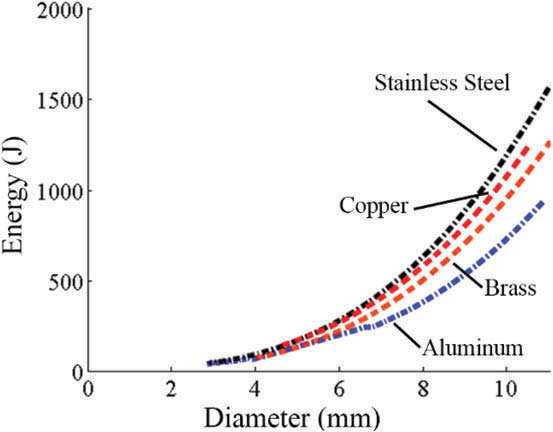
\includegraphics[width=0.5\textwidth]{Figures/particle_ign_boundary.png}
                \caption{Observed ignition boundary, quantified by particle energy, as a function for cellulose powder for various materials and particle sizes from Fernandez-Pello et al.~\cite{Fernandez-Pello2015}.}
                \label{fig:energy_diameter}
            \end{figure}
        Similar results for hot particles were obtained for pine needles by Wang et al.~\cite{Wang2017}, for powdered grass by Urban et al.~\cite{Urban2017}, and again with cellulose by Hadden et al.~\cite{Hadden2011}. While similar trends have been observed across a range of materials using similar energy delivery methods, efforts to create a model to predict ignition boundaries have not been successful. The difficulties preventing an ignition model have stemmed from the lack of knowledge about the ember fuel bed interface, thermal properties of the fuel bed, and difficulties in determining particle heat losses to ambient. 
        
        While observations informing trends that increased energy and heat transfer increase  probability are important, the next step is to quantify the transition or critical values for parameters observed to control the trends. A universally predictable critical value has not yet been determined but, predictive capabilities for single conditions or experimental apparatus have been determined. More detail on what has been learned about the impact of energy deposition and effects of energy deposition on pyrolysis is contained in the following sections.
        
        \subsection{Fuel Moisture Content}
        The presence of water in fuel bed particles, quantified as fuel moisture content, impacts the ignition process in multiple ways. Since the vaporization of water occurs at a lower temperature than pyrolysis, the water in a fuel particle must be evaporated before pyrolysis can occur. This creates a large energy sink for the energy imparted to the fuel bed from an ember or firebrand, thus increasing the amount of energy needed to ignite a fuel bed~\cite{Hurley2016}. Studies have universally shown this to be the case as is described in Table~\ref{tab:binary} rows~\ref{tabrow:wang2017}, \ref{tabrow:ellis2015}, \ref{tabrow:ellis2011}, \ref{tabrow:ganteaume2009}, \ref{tabrow:plucinski2008}, \ref{tabrow:manzello2006}, \ref{tabrow:manzello2006a}, and~\ref{tabrow:dimitrakopoulos2001}. This trend indicates that fuel moisture content is a parameter to be added as a lumped constant to the minimum energy needed to ignite a fuel bed. However, water in the fuel has additional impacts on the pyrolysis and ignition processes. Computational efforts have shown that increasing the moisture content of the fuel decreases both the peak mass loss rate and peak heat release rate of a fuel sample\cite{Shotorban2018}. The decrease in the heat release rate and mass loss rate may have significant effects on the chemical composition of the pyrolysis gases, as was observed by Furgeson et al.~\cite{Ferguson2013} where an increased moisture content shifted the \ce{O2} and \ce{H} concentrations in flames burning pyrolysis gases. It should be noted that this effect was observed for the piloted combustion of pyrolysis gases, but increasing amounts of \ce{H2O} would likely have a similar impact on the auto-ignition of pyrolysis gases. The implications of these effects are discussed further in Section~\ref{subsec:pyrolysis}, as they relate more directly to pyrolysis of the fuel and gas dynamics above the fuel bed. 
        
        In addition to acting as an energy sink for evaporation, increasing the fuel moisture content alters the thermal conductivity of a fuel bed. Tests for the thermal conductivity of wheat showed that a 28\% increase in wheat moisture content increased the thermal conductivity by ~40\%\cite{Tavman1998}. The increased heat diffusion rates would lead to lower temperatures and temperature gradients in the fuel bed, changing the mass flux rate of pyrolyzates departing the fuel bed and the composition of said pyrolyzates. The relative magnitude of increased moisture content in other fuel bed materials is unclear, but a ~40\% shift in thermal conductivity would have significant impacts on the heat diffusion rates from a firebrand delivering energy to the fuel bed.
        Perhaps the most important knowledge gained from the extensive study of fuel moisture content and its impacts is that due to the numerous scales across which ignition of fuel beds occur it is essential to evaluate the impacts of each parameter across all scales since the phenomena may be more closely interdependent than initially observed. 
            
        \subsection{Species and Morphology}
        One of the factors that sets the ignition of fuel beds apart from ignition of other materials is the vast array of species and particle morphology encountered in nature. For example, in a forest with a relatively uniform litter layer, the particle size distribution may range from small pieces of grass to twigs that are an order of magnitude larger. Even a layer of pine needles on a roof will have a distribution of sizes, shape, orientation, and bulk density. On the scale of the fuel bed, the differences in shapes and sizes of the particles ensure that every fuel bed is unique, making repeatability while studying fuel bed ignition difficult at best. 
        
        Implications for fuel bed uniqueness is twofold. First, the differences in particle shape, e.g., pine needles vs oak leaves, cause the heat transfer properties of fuel beds to be highly variable. Second, each species has different composition and fuel beds may consist of many species. Having fuel bed particles of different compositions and morphology in a fuel bed obfuscates the relative effects of individual particle thermal conductivity and inter-particle heat transfer due to contact area and particle shape. Furthermore, a fuel bed with multiple species will undergo a wide array of chemical processes in a single fuel bed when pyrolyzates are generated. Samples of the same fuel have also been shown to have different pyrolyzate composition under differing heating conditions~\cite{Gauthier2013}. For example, decreasing the heating source from 1050$^{\circ}$C to 450$^{\circ}$C reduced the elemental composition of hydrogen in the pyrolysis products by 23\% and increased the elemental composition of oxygen by 28\% on a \% mole basis. The inherent variability in natural fuel bed has limited observations to qualitative trends.
        
        
        Fortunately, despite the large variability across species and materials, there are three major components that are common across most biomass fuels: cellulose, hemicellulose, and lignin. Recent efforts, supported by the large amount of data produced by the previously mentioned studies, have attempted to find a common characterization for biomass materials by comparing composition differences. It was found that characterization of cellulose, hemicellulose, and lignin composition was not sufficient and extractive compounds must be considered. When extractive compounds were considered, chemical kinetic properties were able to be predicted within accuracy of existing models~\cite{Debiagi2015} with more detailed characterizations. This development helps lessen some of the difficulties encountered in previous studies by enabling the comparison of different species with less intensive methods of characterization. The ability for this approach to increase comparability between tests is a significant step forward in the understanding of ignition. However, there remains a multitude of effects on ignition introduced by species and morphology that need to be considered. These effects are outlined and considered in the following section. 
        
        \subsection{Pyrolysis Production and Air Mixing}\label{subsec:pyrolysis}
        Pyrolysis of fuel bed material is the keystone process for the ignition of fuel beds. Once the heat transfer to the fuel bed raises the temperature of the fuel enough for pyrolysis to occur, a number of conditions must be met for the ignition to occur.  The thermal degradation reactions that occur at the onset of pyrolysis are heavily influenced by the parameters discussed in the previous sections. The rate of energy deposition, fuel moisture content, species, and fuel morphology all modify the rate and composition of pyrolysys products. 
        The heating rate and the overall energy imparted to the fuel bed have the most prominent effect on the pyrolysis reactions in a fuel bed. At low temperatures and low heating rates the main components released by the fuel bed consist of chars, tars, and other large hydrocarbon chain molecules due to incomplete breakdown of the materials. As temperatures increase the products shift to more complete reactions that increase the amount of \ce{CO}, \ce{CO2}, \ce{H2}, and small hydrocarbons produced~\cite{Gauthier2013}. An example of this effect is shown in Figure~\ref{fig:temp_effects_pyrolysis} where small wood particles were placed in a heating apparatus at various temperatures. 
            \begin{figure}
                \centering
                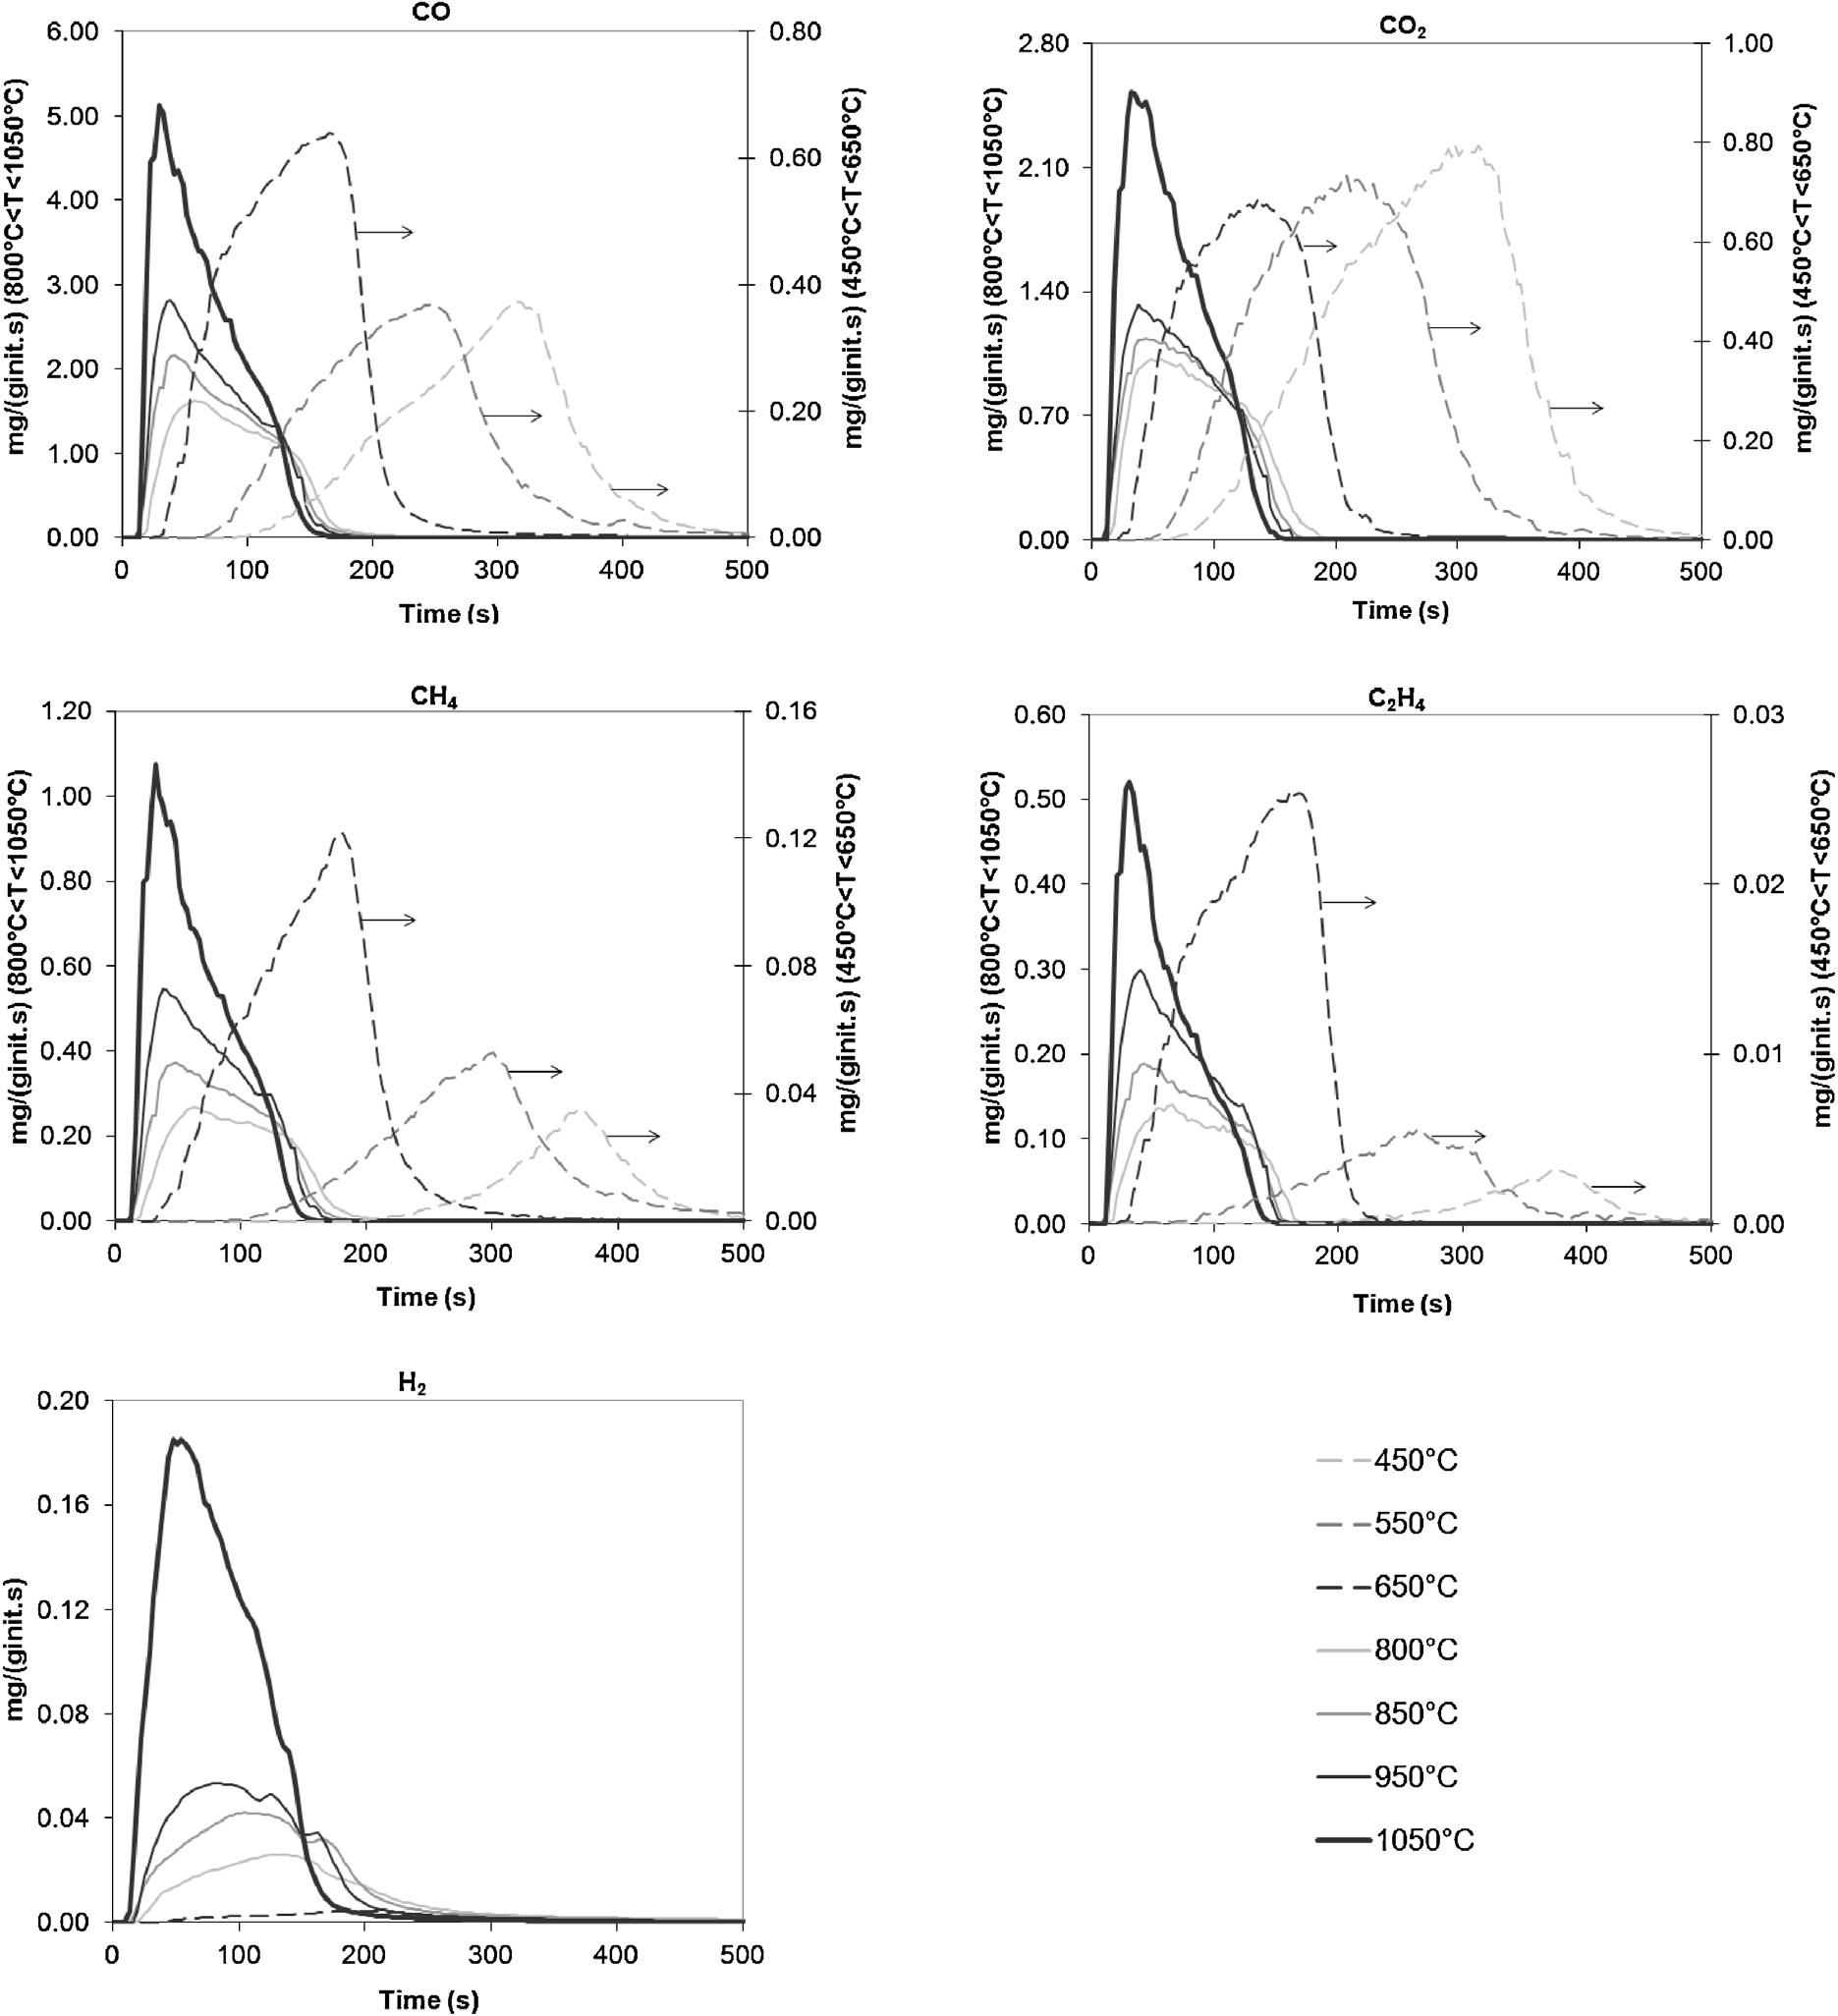
\includegraphics[width=0.75\textwidth]{Figures/gauthier2013_temp_effects.png}
                \caption{Pyrolysis gas concentrations for beech wood samples heated at different rates from ~\cite{Gauthier2013} showing the significant decrease in gas production rates for most gases as the sample temperature decreases.}
                \label{fig:temp_effects_pyrolysis}
            \end{figure}
        As is plotted in Figure~\ref{fig:temp_effects_pyrolysis}, the heating rate affects both the rate of gas productions and the total amount of gas production. These trends have significant implications for ignition of pyrolysis gases above the fuel bed, since auto-ignition is dependent on the temperature, concentration, and species of the gases in the buoyant plume above the fuel bed.
        
        Similar trends have been observed for larger solid plates of plastics and wood in a wind tunnel with piloted flame. It was observed that under higher heat fluxes, the ignition time was shorter but the amount of pyrolyzates generated per time increases. The rate of pyrolyzate generation above which ignition was observed is considered to be the critical mass flux. This phenomena has been observed consistently across plastic and wood plates, as well as pine needles~\cite{McAllister2013, Hernandez2018}. The increase in the critical mass flux for ignition is attributed to higher temperature gradients in the material, causing most of the chemical reactions to occur near the surface of the material at a higher oxygen content and temperature~\cite{Rich2007}. Reactions under these condition produce more \ce{CO} and \ce{CO2}, as shown in Figure~\ref{fig:temp_effects_pyrolysis}, which have a increased lower flammability limit than larger hydrocarbons produced at lower heat fluxes. What is not clear from these findings is how fuel beds of different materials compare to solid fuels under the same conditions or the effects of different heat transfer modes. As particle sizes increase, the properties of the fuel bed become further from a solid as the porosity, surface area, and oxygen availability increase. The converse of these increases is a likely drop in bulk fuel bed thermal conductivity, creating higher temperature gradients. These temperature gradients have been shown to have change pyrolyzate composition for very small sample sizes ($\leq$10mg) in highly controlled Thermogravametric Analysis (TGA) tests~\cite{Richter2018}. While it is apparent that temperature gradients in the fuel bed affect pyrolyzate production, it is unclear how this will effect ignition of the fuel bed on scales found in fires. For these larger fuel beds, distributions of temperature and species concentrations caused by non-uniform and multiple heat sources is an important factor to understand when considering ignition. 
        
        Entrainment and mixing of air with pyrolyzates above the fuel bed has a pronounced effect on the ignition of fuel beds. As shown in Table~\ref{tab:binary} rows~\ref{tabrow:wang2017}, \ref{tabrow:ellis2015}, \ref{tabrow:ellis2011}, \ref{tabrow:plucinski2008} studies of fuel bed ignition that considered variable wind speed reported that an increase in wind speed increased the probability of ignition with other factors held constant. Increasing the flow velocity above the fuel bed reduces both the relative importance of buoyant forces and the timescale for mixing. With increased velocity and turbulence, air and pyrolyzates mix faster but heat loss to increased air advection also increases. The relative magnitude of time scales between heat and species diffusion in reacting flows are commonly compared using the Damkohler number as shown in Equation~\ref{eqn:dam}.
        
            \begin{equation}\label{eqn:dam}
                \text{Da} = \frac{\text{flow time scale}}{\text{chemical time scale}}
            \end{equation}
        In the Damkohler number, the flow velocity and turbulence that affect the mixing of air and pyrolyzates are considered in the flow time scale term.  The chemical time scale term considers the pyrolyzate species concentration and temperature effects. The interaction of these two terms is well defined and commonly used in combustion to determine flame regimes and ignition. Use of the Damkohler number as a relation to define ignition has seen limited use in ignition of fuel beds since the knowledge of species concentrations, temperatures, and air flow effects are largely unknown. Gaining insight into these effects would enable the use of tools like the Damkohler number to successfully predict ignition across a variety of fuel beds. 
        Namely, quantification of the parameters near the fuel bed (e.g., surface wind speed), fuel properties (e.g., chemical composition, estimated ember contact area), and the energy content of a firebrand may enable a common metric to predict if ignition will occur in a fire without ignition testing for a certain specific fuel, set of conditions, and location.
        \subsection{Summary}
        Substantial progress has been made to further the understanding of fuel bed ignition and the effects of various related parameters. Despite these efforts, there remains no universal or even quantitative approach that can be used to effectively predict ignition of fuel beds without prior testing for a specific source or fuel. Current knowledge is capable of predicting ignition of solids and predicting different pyrolysis properties of fuels, but the knowledge has not been extended to fuel beds that may occur in forest fires and near structures. One of the largest gaps in knowledge that remains is to determine how fuel beds that consist of fine fuel particles behave in comparison to solid theory. In addition, the effects of non-uniform heating and variable energy deposition are largely unknown. In order to close these knowledge gaps three avenues of research are proposed. First, the heat transfer properties of the fuel bed must be quantified to obtain better knowledge of how the fuel bed responds to heating. Second, the generation rates of pyrolyzates and the effect that heating rates, heat source temperatures, and heating modes must be quantified. Third, the mixing timescales between the pyrolyzates and air must be evaluated to determine what rate the pyrolyzates must be generated to achieve ignition across a variety of conditions. This approach will help bridge the gap between the fundamental theories for ignition and real fuel beds where wildfires occur. The approach and methodologies for each of these fundamental processes is outlined in the following sections. 
%!TEX root = thesis.tex

\newcommand{\TheTitle}{Sensitivities of Porous Beds and Plates to Ignition by Firebrands}
\renewcommand{\TheAuthors}{Derek Bean, David L. Blunck \\ \\ My contributions to this work included the design of the experiments, fabrication of the experimental apparatus, collecting data and/or supervising undergraduates who collected data, data analysis, conducting modelling efforts, and preparation of the manuscript.}

\newcommand{\TheAddress}{
\textit{Frontiers in Mechanical Engineering} \\
Vol.~7, 1-11, 2021. \\
\doi{10.3389/fmech.2021.653810}
}

\PaperHeader{\chapter{\TheTitle}}{\TheAuthors}{\TheAddress}

\label{part:manuscript1}

\newpage
\section{Abstract}
    The increasing occurrence of severe wildfires, coupled with the expansion of the wildland urban interface has increased the number of structures in danger of being destroyed by wildfires. Ignition by firebrands is a significant avenue for fire spread and structure loss; thus, understanding processes and parameters that control the ignition of fuel beds by firebrands is important for reducing these losses. In this study the effect of fuel bed characteristics (i.e., particle size and porous or solid fuel bed) on ignition behavior was considered.  Modelling and analysis was conducted to better understand parameters that are dominant in controlling ignition. The fuel beds, made from Douglas-fir shavings, Douglas-fir plates, or cardboard plates, were heated with a cartridge heater (i.e., surrogate firebrand) to observe ignition. Smaller particles were observed to ignite more readily in porous beds than larger particles when heat transfer from the heater is primarily through conduction. This occurs in large part due to differences in contact area between the fuel bed and the heater coupled  with thermal properties of the fuel bed. As particle sizes increased, ignition was more likely to occur at extended times (\textgreater 100\si{\second}) due to the increased importance of radiation heat transfer. Douglas-fir plates were primarily observed to ignite at times where conduction was the dominant mode of heat transfer (\textless 10\si{\second}). Heat flux delivered to the fuel bed was observed to be a more accurate predictor of ignition likelihood and ignition time than heater temperatures. The characteristic ratio of transport and chemical timescales can be used, in conjunction with the measured heat flux and thermal diffusivity of the fuel beds, as a first approximation to predict ignition for the porous fuel beds. This suggests that future work focusing on these parameters may produce a general characterization of fuel bed ignition probability across fuel beds materials and morphologies.  

\section{Introduction}
     Increasing urban expansion into the wilderness has increased the area of the wildland urban interface (WUI). The increase of the WUI, coupled with global climate change has resulted in fires of increasing severity, size, and impact to humans. For example, consider the state of California in the United States, where four of the five largest fires and three of the five most destructive fires have occurred in the past decade~\cite{CalFire2019, CALFIRE2018}. These fires highlight a trend in the increasing severity of wildfires. Of particular concern with the increasing severity of wildfires is the severity of fires in the WUI. The 2018 Camp fire, where residential property losses amounted to more than twice the reported costs for nationwide federal suppression efforts during the same year~\cite{USDOI/USDA2019, Insurance2019}, is a stark example of how severe a fire that occurs in the WUI can be. A significant mechanism for the spread of fires into the WUI, or even within the WUI, is the ignition of fuel beds by firebrands~\cite{Mell2010, Maranghides2013NISTIgnitions}. Ignition by firebrands in wildfires occurs when a hot combusting particle is generated within the fire and transported, typically by wind, to a recipient fuel bed~\cite{Koo2010a}. Structures in the WUI often have geometry conducive to the collection of firebrands, further increasing the risk of ignition~\cite{Suzuki2020}. Hence, efforts to mitigate the destruction that can be caused by fires in the WUI must consider the role of ignition by firebrands.
     
    Three primary processes control the ignition of fuel beds by firebrands. Specifically, heat transfer between the fuel bed and the firebrand, pyrolyzate generation in the fuel bed, and the mixing of the pyrolyzates above the bed at sufficient temperatures for ignition to occur \cite{Babrauskas2003}. A recent review of the role of firebrands in the spread of fires by Manzello et al.~\cite{Manzello2020} identified that research into the ignition behavior of fuel beds by firebrands is critical to improving preventative measures. Work conducted by Manzello et al.~\cite{Manzello2006a, Manzello2006, Manzello2008} studying ignition of various fuel bed materials (e.g., cut grass and pine needle beds) concluded that the most influential factors for ignition were the number flux of firebrands to the fuel bed, the size of the firebrands, and the airflow over the fuel bed. Similar conclusions were found by Urban et al.~\cite{Urban2019a}, who found that larger firebrands were more likely to ignite fuel beds (i.e., fine sawdust) across a range of fuel moisture contents. These observations illustrate the critical role of heat transfer to the fuel bed in causing ignition. What is not clear from studies such as these is how ignition behavior would change for fuel beds other than those tested, even if identical firebrands were used. Even how the size of fuel particles alter ignition is not clear. Such knowledge is needed to help transition knowledge to a variety of fuel beds that can be present near the WUI (e.g., wood shavings, needles, leaves, etc.). 
    
    Essential to understanding the ignitablility of fuel beds is understanding how the role of heat transfer and energy of a firebrand influences ignition. Hadden et al.~\cite{Hadden2011} found that as the energy content of hot metal particles increased the ignition probability increased. It was also observed that the particle energy alone is not a sufficient condition for ignition to occur and that a minimum particle temperature is required. Similarly, Zak et al.~\cite{Zak2014} observed that the energy of a metal particle was not a sufficient parameter for ignition and minimum values for particle energy and temperature are required; the values of which are dictated by the ability of hot particles to generate sufficient amounts of hot pyrolyzates in fuel beds. Further studies by Fernandez-Pello et al.~\cite{Fernandez-Pello2015} added to the understanding of these factors concluding that heat losses from the hot particle, which reduce the heat flux to the fuel bed, can have a significant impact on the ignition of fuel beds. Additional studies conducted by Urban et al.~\cite{Urban2017, Urban2018} found that the timescale of flaming ignition can be relatively short ($\le$ 100 ms).  Furthermore, smaller fuel bed particles tended to ignite at lower metal particle temperatures. A sensitivity of ignition to the chemical composition of the fuel bed was also observed. While sensitivities to fuel bed particle size, ember particle size, and ember energy have been observed, the relative effect of each parameter on ignition limits and a general application of these sensitivities across various fuel beds and embers remains elusive. 
    
    Studies evaluating the heat flux of firebrands and the critical heat flux for ignition have yielded further insights into the ignition process. Hakes et al.~\cite{Hakes2019a} found that, for a single cylindrical firebrand and piles of firebrands, peak heat flux values ranged between 20 and 60 \si{\kilo\watt\per\square\meter} with average heat fluxes between 12 and 25 \si{\kilo\watt\per\square\meter}. The mass of the firebrands or piles of firebrands had little effect on the peak heat flux but directly influenced the total energy released. Tao et al.~\cite{Tao2020} observed similar heat fluxes for various of natural and manufactured firebrands. Both Hakes et al.~\cite{Hakes2019a} and Tao et al.~\cite{Tao2020} observed that an increase in wind speed significantly increased the measured heat flux. Hernandez et al.~\cite{Hernandez2017} found that Monterey Pine (\textit{pinus radiata}) needles ignited under heat flux as low as 10 \si{\kilo\watt\per\square\meter} with ignition time decreasing proportionally to the inverse square of increasing heat flux. In similar tests but with different fuels, Rivera et al.~\cite{Rivera2020} observed that critical heat fluxes for ignition were highly dependent on fuel bed properties with the critical radiative heat flux increasing as the porosity decreased. Reported critical values ranged from 6.64 \si{\kilo\watt\per\square\meter} to 20.85\si{\kilo\watt\per\square\meter} for Monterey Pine needles with porosities of 0.09 and 0.01, respectively. It has been observed that a variety of firebrands are capable of producing heat fluxes well above the critical heat flux values long enough for ignition in some fuels. However, upon comparing these values to other studies, ignition is not guaranteed if the critical heat flux rate and duration are met. For example, experiments conducted by Manzello et al.~\cite{Manzello2008} used firebrands similar to Hakes et al.~\cite{Hakes2019a} and Tao et al.~\cite{Tao2020} with fuels similar to Hernandez et al.~\cite{Hernandez2017} and Rivera et al.~\cite{Rivera2020} (e.g., wooden disks on pine needles) but did not observe ignition under conditions that would be anticipated to produce ignition. It should be noted that the studies conducted by Hernandez et al. and Rivera et al. were conducted under quiescent conditions and those by Manzello et al. between 0.5\si{\meter\per\second} and 1.0\si{\meter\per\second}. Nevertheless, the reported values of firebrand heat flux at 0.5\si{\meter\per\second} and 1.2\si{\meter\per\second} conditions by Tao et al. suggest ignition is likely to occur for instances where no ignition was observed. Not observing ignition under conditions at the apparent intersection of these findings suggests that other factors may be as important as heat flux and duration of heating. 

    Given this background and motivation the objective of this work is to identify how the size of fuel particles influences ignition and to ascertain changes in ignition of porous and solid fuels. Time to ignition tests with a cartridge heater were conducted to elucidate this sensitivity. It is anticipated that the observations from this study will enhance the understanding of fuel bed ignition and enable more focused studies regarding additional effects of fuel bed properties on ignition. 
  
 
\section{Methodology}
   The time to ignition was measured for five different fuel bed conditions with varying surface temperatures of a resistance heater.  The time to ignition was the metric used to evaluate the ignition propensity. The experimental apparatus, as illustrated in Figure~\ref{fig:ignPropensity}, was designed to replicate both conduction and radiation that may occur when a firebrand lands on the fuel bed. The heater was held in place by a lever arm that, when lowered, positioned the heater at a fixed location for the duration of the test. The firebrand was represented by a 6.35\si{\milli\meter} diameter 51\si{\milli\meter} long cartridge heater capable of a 250\si{\watt} output. The heater was inserted 3\si{\milli\meter} into the bed (approximately half the diameter) in the porous media tests and on top of the plates for the other experiments. The temperature of the heater was continually recorded via a type-K thermocouple attached to the top of the heater. An important distinction between using the lever arm holder and a naturally occurring firebrand is that the location of the heater remained fixed and, for times greater than roughly 10\si{\second}, could lose contact with the fuel bed as material was lost because of pyrolysis.  Thus, for the longer ignition experiments the arrangement mimicked a firebrand with a gap between it and the fuel bed, instead of a firebrand that maintained consistent contact. The rationale in using the lever arm was to ensure that the heater was placed a consistent depth within the fuel bed since sensitivities of ignition to heat source penetration depth have been observed by Wang et al.~\cite{Wang2016}. The temperature of the heater was held to within $\pm$ 6\% of the set point using PID control implemented in LabVIEW. Power delivery to the heater was measured at a rate of 1kHz for all tests. 
   Admittedly, the temperature and heat transfer from an actual firebrand to a fuel bed may vary more than that of a controlled heater, nor does the heater have a piloted ignition source. Nonetheless, trends of ignition propensity are expected to be similar between the heater and firebrands since the heat transfer rates calculated in these experiments are in the range of 1\si{\kilo\watt\per\square\meter} to 21\si{\kilo\watt\per\square\meter} which are comparable to heat flux values reported by Hakes et al.~\cite{Hakes2019a} and Tao et al.~\cite{Tao2020} for combustion of glowing firebrands on an instrumented surface. The advantage of using a heater was that it allowed sensitivities of ignition to the fuel beds and controlling processes to more readily be identified because the boundary conditions were measured, controlled, and consistent.
   
    Wood particles and flat plates were used as the fuel bed materials. The fuel particles were Douglas-fir (\textit{Pseudotsuga menziesii}) shavings sorted into three size classes: $L_{c}<$1\si{\milli\meter}, 4\si{\milli\meter} $<L_{c}<$ 6\si{\milli\meter}, and 6\si{\milli\meter} $<L_{c}<$ 12\si{\milli\meter} to allow sensitivities of ignition to be identified. Fuel particles were generated by processing Douglas-fir lumber through a planer and then sorted by screening and/or granulating to achieve the desired size distribution. The fuels were placed in a glass container with a diameter 140\si{\milli\meter} and a depth of 70\si{\milli\meter}. The container was filled to the rim for the porous media tests, but the fuels were not packed. The materials used for the tests with flat plates were Douglas-fir and corrugated cardboard processed into 75\si{\milli\meter}-by-75\si{\milli\meter} squares. The thickness of the Douglas-fir and cardboard plates were 5\si{\milli\meter} and 6\si{\milli\meter} respectively. For plate ignition tests, the plates were stacked in the container to be level with the rim, replicating the porous media tests as close as possible.
   
    The time to ignition was determined from the signal emitted from a BPX65 photodiode positioned to capture the lowering of the cartridge heater and the flames resulting from ignition. This measurement approach only considered flaming ignition. The time to ignition was defined as the time between the maximum light intensity gradients, which corresponds to lowering the heater onto the fuel bed and the ignition event. The photodiode was sampled at 1kHz. Consistency in airflow, and thus oxygen availability, was achieved by maintaining the apparatus in the same orientation in a fume hood with the same airflow settings for every test. The average air velocity over the fuel bed was measured using a hot wire anemometer (TSI IFA300). Measurements were taken with the sample bowl filled with fuel particles and the heater in the lowered testing position at room temperature with the probe positioned approximately 16\si{\milli\meter} above the fuel bed. The average air velocity over the fuel bed was 0.1\si{\meter\per\second}.
        \begin{figure}[htpb]
            \centering
            \resizebox{\figureWidthSet}{!}{%
            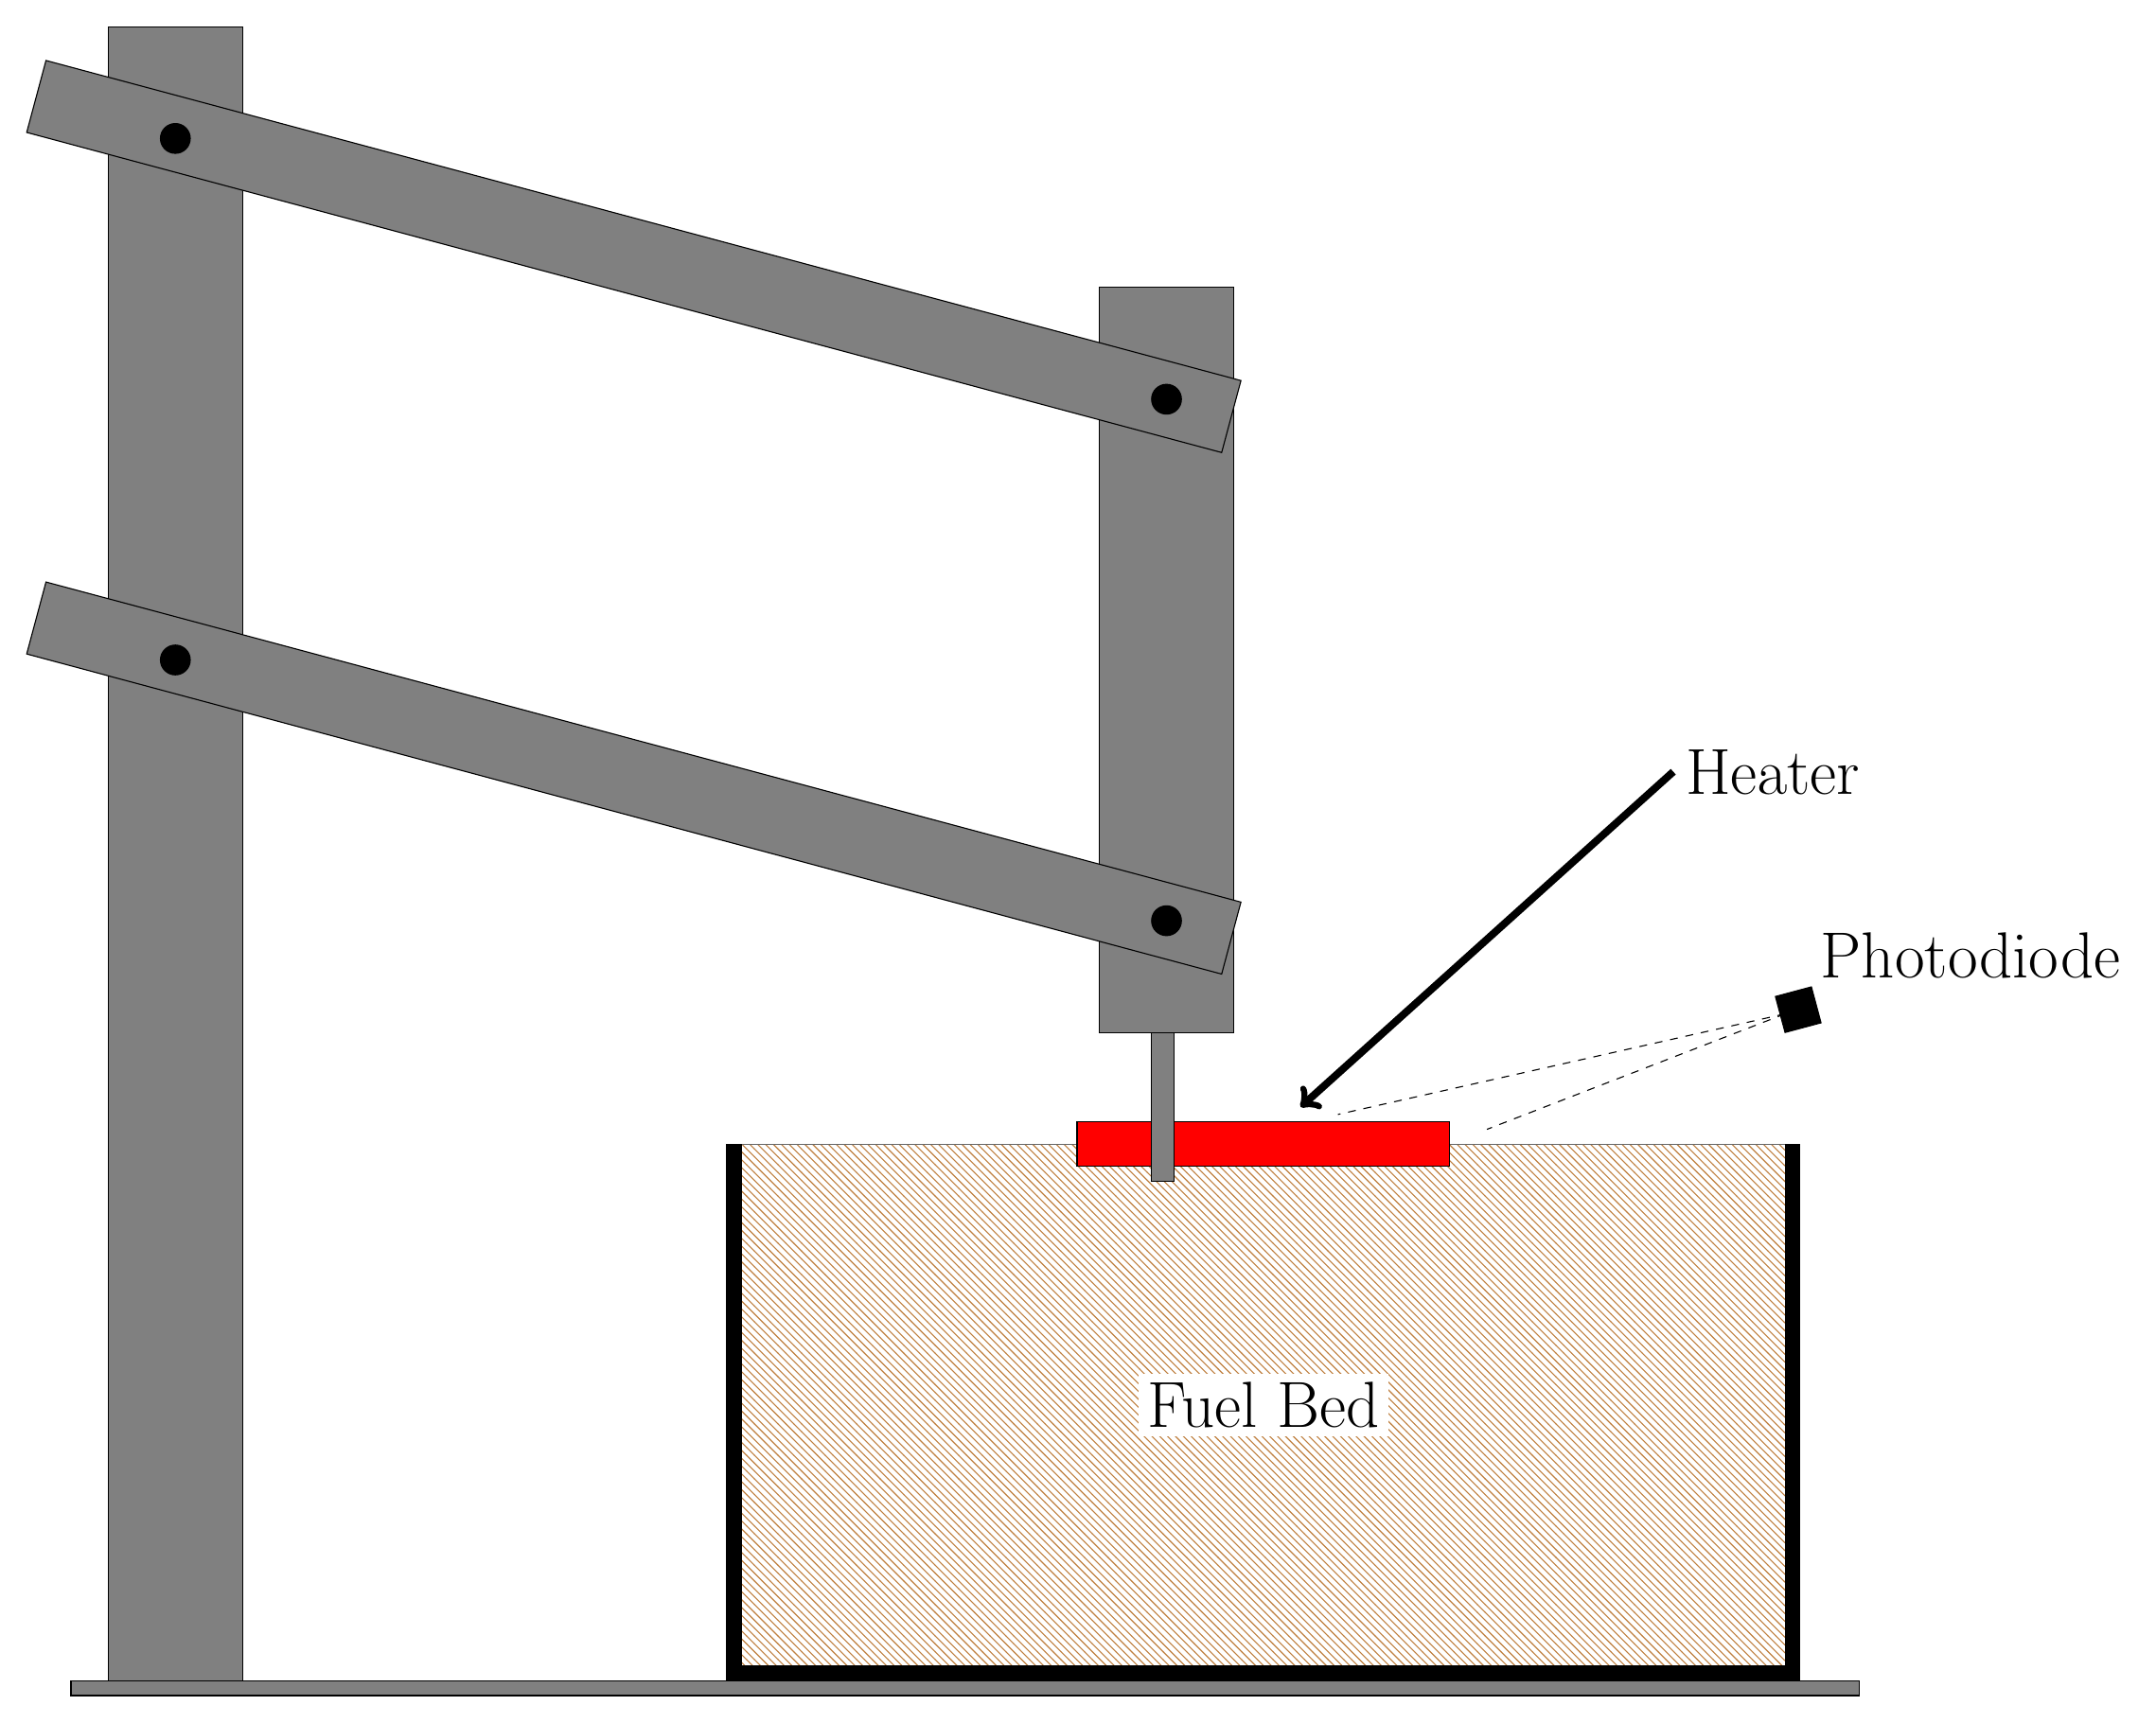
\begin{tikzpicture}
                \filldraw [draw=black!60, pattern=north west lines, pattern color= brown] (0, 0) rectangle (140mm, 70mm) node[pos=0.5, fill=white] {\Huge Fuel Bed}; 
                \filldraw[] (0mm, -2mm) rectangle (140mm,0mm) node[rotate=-90, pos=0.5] {};
                \filldraw[] (-2mm, -2mm) rectangle (0mm,70mm) node[rotate=-90, pos=0.5] {};
                \filldraw[] (140mm, 70mm) rectangle (142mm,-2mm) node[rotate=-90, pos=0.5] {};
                \filldraw [fill=red, draw=black] (45mm, 67mm) rectangle (95mm, 73mm) {}; 
                \filldraw [draw=black, fill=black!50] (55mm, 65mm) rectangle (58mm, 85mm) {};
                \filldraw [draw=black, fill=black!50] (66mm, 85mm) rectangle (48mm, 185mm) {};
                \filldraw [draw=black, fill=black!50] (-85mm, 220mm) rectangle (-67mm, -2mm) {};
                \filldraw [draw=black, fill=black!50, rotate around={-15:(57mm, 100mm)}] (66mm, 95mm) rectangle (-100mm, 105mm) {};
                \filldraw [draw=black, fill=black!50, rotate around={-15:(57mm, 170mm)}] (66mm, 165mm) rectangle (-100mm, 175mm) {};
                \filldraw [draw=black, fill=black!50] (-90mm, -2mm) rectangle (150mm, -4mm) {};
                \filldraw (57mm, 170mm) circle (2mm);
                \filldraw (57mm, 100mm) circle (2mm);
                \filldraw (-76mm, 205mm) circle (2mm);
                \filldraw (-76mm, 135mm) circle (2mm);
                \filldraw [rotate around={15:(140mm, 85mm)}] (140mm, 85mm) rectangle (145mm, 90mm) node[above right] {\Huge Photodiode};
                \draw [<-, line width=1mm] (75mm, 75mm) -- (125mm, 120mm) node[right] {\Huge Heater};
                \draw [dashed] (140mm, 87.5mm) -- (100mm, 72mm);
                \draw [dashed] (140mm, 87.5mm) -- (80mm, 74mm);
            \end{tikzpicture}
            }
            \caption{Experimental apparatus for the ignition propensity tests. The lever arm used to lower the apparatus into the fuel bed, the fuel bed size relative to the heater, and the location of the photodiode are illustrated.}
            \label{fig:ignPropensity}
        \end{figure}

        % An example photodiode trace is shown in Figure~\ref{fig:photoTrace} where the raw signal, the filtered signal, and the gradient of the filtered signal are shown. 
        % \begin{figure}[htbp]
        %     \begin{center}
        %     \begin{tikzpicture}
        %     \node[anchor=south west,inner sep=0] (image) at (0,0) {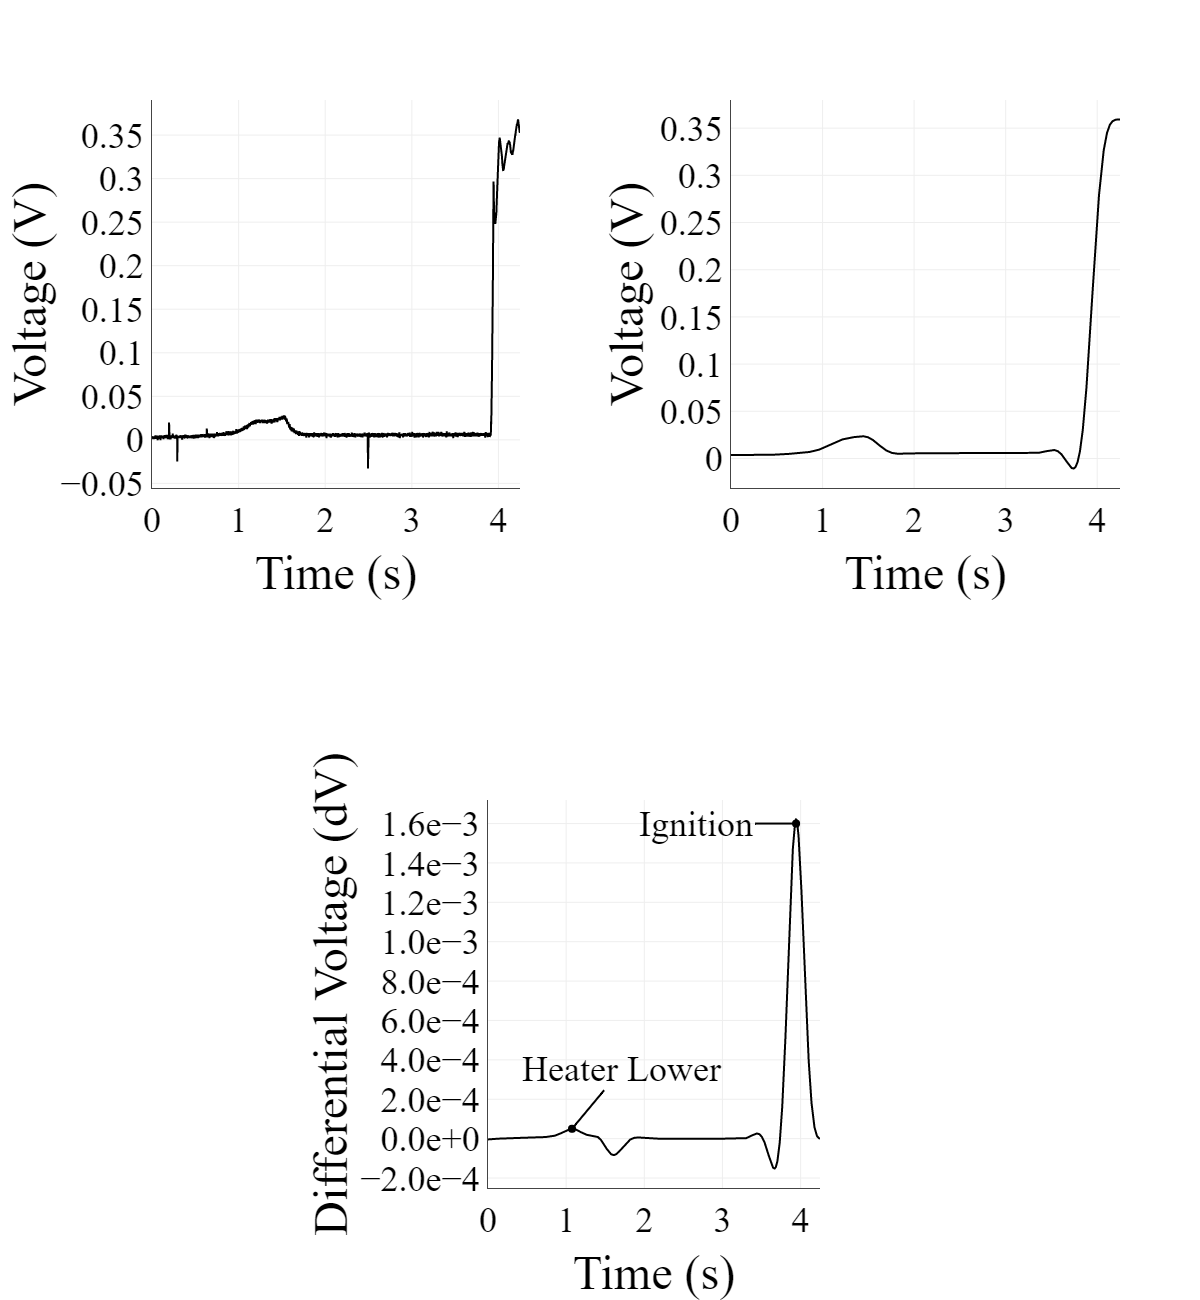
\includegraphics[width=\figureWidthSet]{Figures/stacked_photodiode.png}};
        %         \begin{scope}[x={(image.south east)},y={(image.north west)}]
        %             \node at (0.26, 0.5) {(A)};
        %             \node at (0.75, 0.5) {(B)};
        %             \node at (0.5, -0.03) {(C)};
        %         \end{scope}
        %     \end{tikzpicture}
        %     \end{center}
        %     \caption{Sample photodiode trace showing the signal in the three stages of analysis., \textbf{(A)} Raw Signal, \textbf{(B)} Filtered Signal, and \textbf{(C)} Signal Derivative}\label{fig:photoTrace}
        % \end{figure}

       
    The heat transfer to the fuel bed was estimated by applying an energy balance around the heater using the supplied (measured) power to the heater and subtracting the calculated infrared radiation losses to the surroundings. The heat flux was determined by normalizing the heat transfer to the heater by one-half of the surface area of the heater.  This surface area was justified as the heater was inserted to a depth of half the diameter for each test. Heat loss to the surroundings was estimated by measuring temperatures along the length of the heater but with no fuel bed material in the apparatus. These temperature profiles were then used to estimate the heat losses to the ambient. The emissivity of the heater was taken to be 0.60~\cite{Watlow2020}. Heat flux values were calculated as an average for the duration of the test, and for a 200\si{\milli\second} window when the heater made contact with the fuel bed. These two time scales allowed differences in sensitivities between average and initial heat flux to be observed. The heat flux values provide insights into variations in the characteristic rate of heat transfer from the heater to the fuel bed for each of the materials tested. Combining the heat flux for each material with the estimated thermal conductivity of the fuel bed enabled representative temperature distributions within the fuel bed to be determined. It is acknowledged that the processes addressed in this work are transient, thus the thermal diffusivity of the materials is applicable. However, thermal conductivity is considered here because the calculation of the thermal conductivity relies on fewer correlations and is potentially more accurate. Additionally, the thermal properties of the materials are derived from literature such that both properties are directly proportional to the experimentally obtained bulk density. Thermal conductivity of the fuel bed materials were estimated using the mean of minimum and maximum effective thermal conductivity correlations in porous media~\cite{bergman2011fundamentals}. The correlation for effective thermal conductivity is shown in Equation~\ref{eqn:estk} where $\epsilon$ is defined as the proportion of volume occupied by air, as is shown in Equation~\ref{eqn:epsilon}. 
        \begin{equation}
            k_{eff} = \frac{1}{2} \left(\frac{1}{\left( 1 - \epsilon \right)/k_{solid} + \epsilon/k_{air}} +  \epsilon k_{air} + \left(1-\epsilon \right) k_{solid} \right)
            \label{eqn:estk}
        \end{equation}
        \begin{equation}
            \epsilon = 1- \frac{\rho_{solid}}{\rho_{bed}}
            \label{eqn:epsilon}
        \end{equation}
    The thermal conductivity of Douglas-fir plates and corrugated cardboard plates were obtained from literature~\cite{Laboratory2010, Asdrubali2015}. The bulk density of the porous material ($\rho_{porous}$) and the solid ($\rho_{solid}$) were obtained from experimental samples. Table~\ref{tab:k_values} shows the mean bulk density for each material and the corresponding estimated thermal conductivity values for the porous materials and the solid plates. The values shown in Table~\ref{tab:k_values} were used as inputs to the computational models, as discussed later. 
        \rowcolors{2}{gray!25}{white}
        \begin{table}[hpbt]
            \caption{Measured ($\bar{\rho}$) and estimated (k) fuel bed properties}
            \centering
            \begin{tabular}{crr}
                \rowcolor{gray!50}
                Material & $\bar{\rho}$ (\si{\kilo\gram\per\cubic\meter}) & k (\si{\watt\per\meter\per\kelvin}) \\
                \hline
                Douglas-fir plates  & 510   & 0.120 \\
                $L_{c}<$1mm         & 135   & 0.042 \\
                4mm $<L_{c}<$ 6mm   & 69.9  & 0.034 \\
                6mm $<L_{c}<$ 12mm  & 36.9  & 0.030 \\
                Cardboard plates    & 115   & 0.053
            \end{tabular}
            \label{tab:k_values}
        \end{table}

    Three simplified models were implemented to obtain further insights into the physical and chemical processes causing trends observed in the experimental ignition efforts.
    First, the temperature evolution of the fuel bed was modeled. Second, the time-averaged mass flux and species concentrations of the pyrolysis species leaving the fuel bed and entering the air were estimated using the calculated temperatures of the fuel bed. Third, the ignition delay times of the gaseous pyrolysis species estimated to depart the fuel bed were calculated. Time-averaged and spatially constant values were used for mass flux and mass fraction of pyrolysis products leaving the fuel bed. Figure~\ref{fig:domains} shows the computational domain representing the fuel bed. Figure~\ref{fig:comp_flow} shows the data flow between the models where the rectangles indicate the implementation of a model or calculation, ellipses indicate an output of interest, and the rounded rectangles indicate an input from measurements or literature values. The dotted and dashed boxes outline which calculations pertain to each chemical mechanism used and the overlap shows the information that is transferred between the models. The fuel bed temperature was modeled using OpenFOAM~\cite{Foundation2020}. Modeling of the pyrolysis was conducted using Cantera~\cite{Goodwin2020} with the BioPOx mechanism~\cite{Dhahak2019}. The Bio1412 mechanism~\cite{Ranzi2008, Ranzi2001} was used for gas phase species exiting the fuel bed. The Bio1412 mechanism contains 137 species and 4533 reactions. The BioPox mechanism contains 710 species, 5035 reactions and includes both primary pyrolysis and secondary pyrolysis. The inclusion of secondary pyrolysis is important for the combustion of products in the fuel beds studied since the particle fuel beds contain air that may affect the composition of gases as they leave the fuel bed. 

        \begin{figure}
        \centering
        \resizebox{0.25\textwidth}{!}{%
          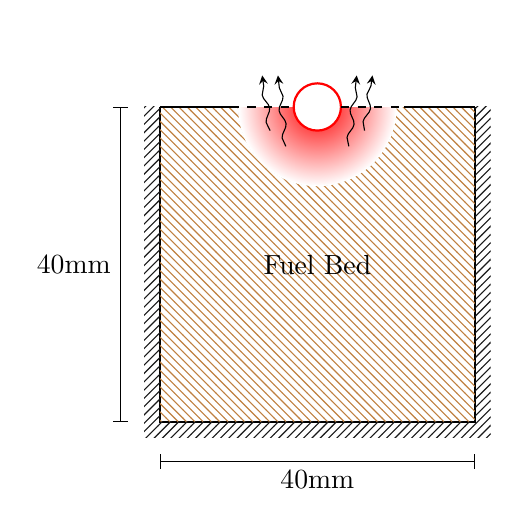
\begin{tikzpicture}
            \node at (0,0) (origin) {};
            \node at (40mm, 40mm) (topright) {};
            %\draw (origin) rectangle (topright);
            \draw [thick] (0mm, 40mm) -- (0mm,0mm) -- (40mm, 0mm) -- (40mm, 40mm);
            
            \fill [pattern=north west lines, pattern color= brown] (origin) rectangle (40mm, 40mm) node[pos=0.5] {Fuel Bed}; 
            \fill [draw=white,  inner color=red, outer color=white ] (20mm, 40mm) circle (10mm);
            \fill[fill=white] (8mm, 40mm) rectangle (32mm, 50mm);
            \filldraw [fill=white, draw=red, thick] (20mm, 40mm) circle (3mm);
            \draw [thick] (0, 40mm) -- (9mm, 40mm);
            \draw [thick, dashed] (9mm, 40mm) -- (17mm, 40mm);
            \draw [thick, dashed] (23mm, 40mm) -- (31mm, 40mm);
  
            \draw [thick](31mm, 40mm) -- (40mm,40mm);
            \fill[pattern=north east lines, pattern color=black!90] (-2mm,-2mm) rectangle (0mm,40mm) node[rotate=-90, pos=0.5] {};
            \fill[pattern=north east lines, pattern color=black!90] (0mm,-2mm) rectangle (40mm,0mm) node[rotate=-90, pos=0.5] {};
            \fill[pattern=north east lines, pattern color=black!90] (40mm, -2mm) rectangle (42mm,40mm) node[rotate=-90, pos=0.5] {};

            
            \draw[-stealth,decorate,decoration={snake,amplitude=1pt,pre length=0pt,post length=2pt}] (16mm, 35mm) -- ++(-1mm, 9mm);
            \draw[-stealth,decorate,decoration={snake,amplitude=1pt,pre length=0pt,post length=2pt}] (14mm, 37mm) -- ++(-1mm, 7mm);
            
            \draw[-stealth,decorate,decoration={snake,amplitude=1pt,pre length=0pt,post length=2pt}] (24mm, 35mm) -- ++(1mm, 9mm);
            \draw[-stealth,decorate,decoration={snake,amplitude=1pt,pre length=0pt,post length=2pt}] (26mm, 37mm) -- ++(1mm, 7mm);
            
            \draw [|-|] (0mm, -5mm) -- (40mm, -5mm) node[pos=0.5, below] {40mm} ;
            \draw [|-|] (-5mm, 0mm) -- (-5mm, 40mm) node[pos=0.5, left] {40mm} ;
          \end{tikzpicture}
          }
        \caption{Diagram of the computational domain where black lines indicate domain boundaries, and red lines are boundaries defined by the heater. The arrows denote flow of pyrolysis products from the fuel bed into the air above the fuel bed.}
        \label{fig:domains}
    \end{figure}
    % go through the flow chart and talk about all of the steps
   
    Modeling of the temperature evolution of the fuel bed was implemented to represent what occurs during the experiments. The domain size for the fuel bed was 40\si{\milli\meter} wide and 40\si{\milli\meter} in depth and ensured that wall effects did not influence the heat transfer over the 10\si{\second} of simulations. The 10\si{\second} time limit was chosen since the majority of experimental ignitions occurred before 10\si{\second}, as explained shortly. Additionally, it was observed in experiments that the fuel bed began to lose contact with the heater beginning near 10\si{\second}, potentially reducing the applicability of the model beyond this time. All sides of the fuel bed domain were treated as insulated, aside from the heater interface. The insulated sides and bottom of the domain are representative of experimental conditions, but the insulated top surface does not account for losses due to convection or radiation from the fuel bed materials.  Nonetheless the calculated temperature distribution within the fuel beds are expected to be valid because heat transfer is dominated by conduction. Reactions and mass loss are not considered in determining the temperature distributions of the fuel beds. Despite these limitations, the calculated temperature distributions provide insights into the mass of each fuel bed material that undergoes pyryolysis which in turn is used for understanding the experimental results.

        \begin{figure}
        \centering
         \resizebox{\figureWidthSet}{!}{%
        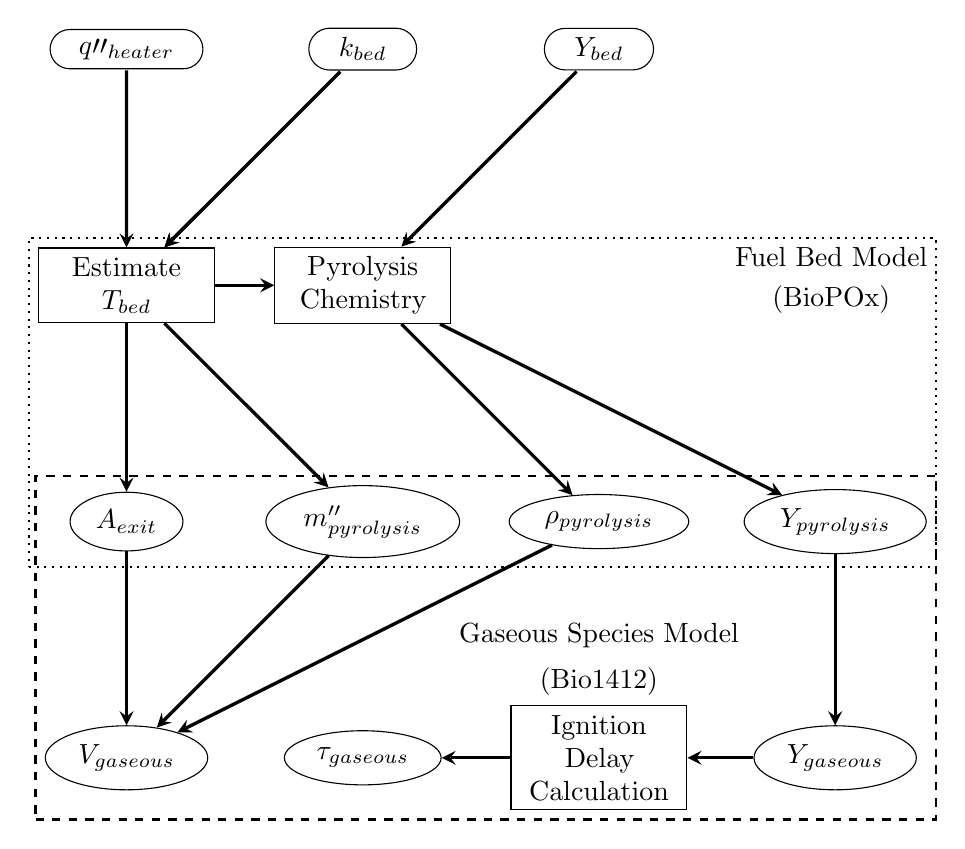
\begin{tikzpicture}[node distance=3cm and 1cm]
            \node (tbed) [draw, process, text width=2cm, text centered ] {Estimate $T_{bed}$};
            \node (qprime) [draw, terminal, above of=tbed] {$q\prime\prime_{heater}$};
            \node (kbed) [draw, terminal, right of=qprime] {$k_{bed}$};
            \node (ybed) [draw, terminal, right of=kbed] {$Y_{bed}$};
            \node (pchem) [draw, process, right of=tbed, text width=2cm, text centered] {Pyrolysis Chemistry};
            \node (aexit) [draw, ellipse, below of=tbed] {$A_{exit}$};
            \node (mflux) [draw, ellipse, right of=aexit] {$m^{\prime \prime}_{pyrolysis}$};
            \node (rhogas) [draw, ellipse, right of=mflux] {$\rho_{pyrolysis}$};
            \node (yprod) [draw, ellipse, right of=rhogas] {$Y_{pyrolysis}$};
            \node (vgas) [draw, ellipse, below of=aexit] {$V_{gaseous}$};

            \node (ygas) [draw, ellipse, below of=yprod] {$Y_{gaseous}$};
            \node (flowsim) [draw, process, left of = ygas, text width=2cm, text centered] {Ignition Delay Calculation};
            \node (tgas) [draw, ellipse, left of=flowsim] {$\tau_{gaseous}$};
            \node [fit=(tbed) (yprod) (mflux),draw,dotted, black, thick] (fuelfit) {};
            \node (FBM) [below left] at (fuelfit.north east) {Fuel Bed Model};
            \node [below] at (FBM.south) {(BioPOx)};
            \node [fit=(aexit) (vgas) (mflux) (tgas) (yprod) (flowsim),draw,dashed,black, thick] (gasfit) {};
            \node (QAM)[above] at (flowsim.north) {(Bio1412)};
            \node [above] at (QAM.north) {Gaseous Species Model};
            \draw [arrow] (kbed) -- (tbed);
            \draw [arrow] (qprime) -- (tbed);
            \draw [arrow] (tbed) -- (pchem);
            \draw [arrow] (tbed) -- (mflux);
            \draw [arrow] (tbed) -- (aexit);
            \draw [arrow] (kbed) -- (tbed);
            \draw [arrow] (ybed) -- (pchem);
            \draw [arrow] (pchem) -- (rhogas);
            \draw [arrow] (pchem) -- (yprod);
            \draw [arrow] (rhogas) -- (vgas);
            \draw [arrow] (mflux) -- (vgas);
            \draw [arrow] (aexit) -- (vgas);
            \draw [arrow] (yprod) -- (ygas);
            \draw [arrow] (flowsim) -- (tgas);
            \draw [arrow] (ygas) -- (flowsim);
        \end{tikzpicture}
        }
        \caption{Illustration of the model used for the estimated heater flux ($q_{heater}^{\prime \prime}$), thermal conductivity of the fuel bed ($k_{bed}$), and chemical composition of the fuel bed ($Y_{bed}$), (e.g., cellulose)  to calculate temperature ($T$) and pyrolyzate distribution above the fuel bed, and determine the resulting ignition delay times($\tau$). Here the subscript $bed$ represents the properties of the fuel bed materials and $pyrolysis$ represents the pyrolysis products leaving the fuel bed and entering the air above the fuel bed. For example, $V_{pyrolysis}$ represents the velocity of pyrolysis gases leaving the fuel bed and entering the quiescent air domain.}
        \label{fig:comp_flow}
    \end{figure}
    
     Combustion of the fuel bed materials was considered in two steps. Reactions occurring within the domain of the fuel bed were characterized with the BioPOx mechanism to include both pyrolysis and gas phase reactions. Reactions occurring at the exit of the fuel bed were considered solely gas phase, thus the Bio1412 mechanism was used. Chemistry calculations for both domains were performed in Cantera. A detailed chemistry model was considered to best capture the physics of the ignition process. However, a detailed discussion of differences in chemistry leading up to ignition are beyond the scope of this work. Instead, this work focuses on qualitative insights into ignition behavior. The mass of the fuel bed undergoing pyrolysis was defined as the mass of the fuel bed material above 220\si{\celsius}. 220\si{\celsius} was selected as it corresponds to the onset of hemicellulose pyrolysis~\cite{Yang2007} and is the lowest temperature estimated for reactions to occur encapsulating the potential breakdown of all constituents. The temperature at which pyrolysis occurred was taken as the average temperature of the fuel bed material above the temperature threshold. This step was necessary since the Cantera calculations performed were 0D. This approach provided an estimate of the average mass per unit time undergoing pyrolysis reactions. The exit area of the pyrolysis products was assumed to be constant for the duration of the test and was defined by the surface area of the fuel bed adjacent to the heater above the pyrolysis temperature at 10\si{\second}. Species were anticipated to depart the fuel bed and participate in gas phase reactions if they were included in both mechanisms. The mass flux of species departing the fuel bed was defined as the mass fraction of the gas phase species in the fuel bed relative to the mass of the fuel bed undergoing pyrolysis (T\textgreater220\si{\celsius}) divided by the surface area of the fuel bed above the pyrolysis temperature as shown by the dashed lines in Figure~\ref{fig:domains}. While in a physical experiment the mass flux and exit area would vary with time, all materials were treated equally in this study for simplicity and consistency in generating and understanding trends.
        
\section{Results}
   The time required for flaming ignition to occur for the various fuel beds is shown in Figure~\ref{fig:ignTime} as a function of heater set point temperature. Four observations are noted. First, the ignition times generally occurred  within the first 10\si{\second}.  If ignition did not occur after 10\si{\second} then it would typically take between 100\si{\second} and 1000\si{\second} to ignite, if at all. Conditions where ignition did not occur are not included in Figure~\ref{fig:ignTime}. A histogram of ignition times and the probability density for each material are shown in Figure~\ref{fig:ignHist} to further quantify the distribution of ignition times. The probability density of the $L_{c}<$ 1\si{\milli\meter} fuel particles, Douglas-fir plates, and cardboard plates are normally distributed with centers at 2.3\si{\second}, 2.8\si{\second}, and 3.9\si{\second}. The $L_{c}<$ 1\si{\milli\meter} fuel particles have an outlier peak centered at 1000\si{\second}. The 4\si{\milli\meter} $<L_{c}<$ 6\si{\milli\meter} and 6\si{\milli\meter} $<L_{c}<$ 12\si{\milli\meter} fuel particles are bimodal with highest density peaks at 1.7\si{\second} and 113\si{\second} respectively. The secondary peaks occur at 113\si{\second} for the 4\si{\milli\meter} $<L_{c}<$ 6\si{\milli\meter} fuel particles and 2.1\si{\second} for the 6\si{\milli\meter} $<L_{c}<$ 12\si{\milli\meter} fuel particles. Second, the probability of ignition at extended times increased as the particle sizes increased. Specifically, the proportion of ignition events in where $t_{ign} <$ 10\si{\second} group were 90\%, 77\%, and 47\% for the particles $L_{c}<$ 1\si{\milli\meter}, 4\si{\milli\meter} $<L_{c}<$ 6\si{\milli\meter}, and 6\si{\milli\meter} $<L_{c}<$ 12\si{\milli\meter} particle sizes, respectively. The third observation is that ignition was not observed beyond 100s for either of the solid plate fuel bed materials. Trends in ignition times for the plates were most similar to those for beds with the smallest particles. Fourth, for the ignition events that occurred within the first 10\si{\second} there is no apparent relationship between time to ignition, temperature, particle size, and fuel bed type. Additionally, the long timescales of some ignition events suggest that smoldering initiates and then transitions to flaming combustion. Since the incidence of ignition at extended times increases as the particle size increases the potential for smoldering to flaming transition is attributed to thermal and physical properties of the fuel bed. The different sensitivities of ignition just described are attributed to differences in the bulk thermal properties, the interface between the heater and fuel bed, and the global equivalence ratio of the fuel bed, as explained later. 
        \begin{figure}[htp]
            \centering
            \begin{tikzpicture}
                \node[anchor=south west,inner sep=0] (image) at (0,0) {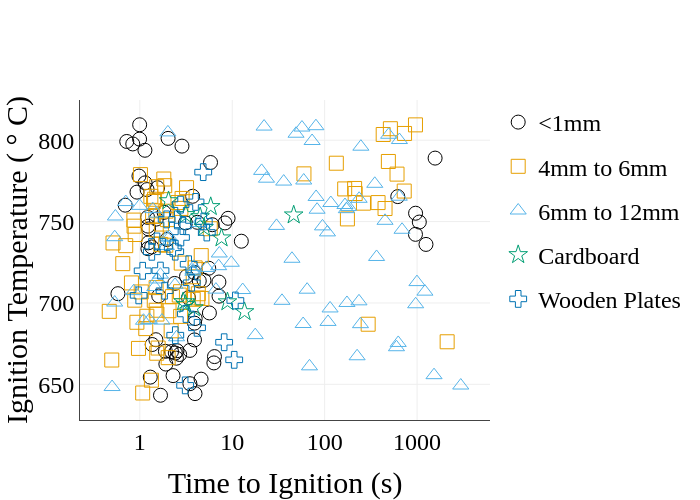
\includegraphics[width=\figureWidthSet]{Figures/ignition_comparison.png}};
                    \begin{scope}[x={(image.south east)},y={(image.north west)}]
                        \draw[dashed, thick,rounded corners] (0.12, 0.17) rectangle (0.33, 0.80);
                        \draw[dotted, thick,rounded corners] (0.46, 0.17) rectangle (0.68, 0.80);
                    \end{scope}
            \end{tikzpicture}
            % 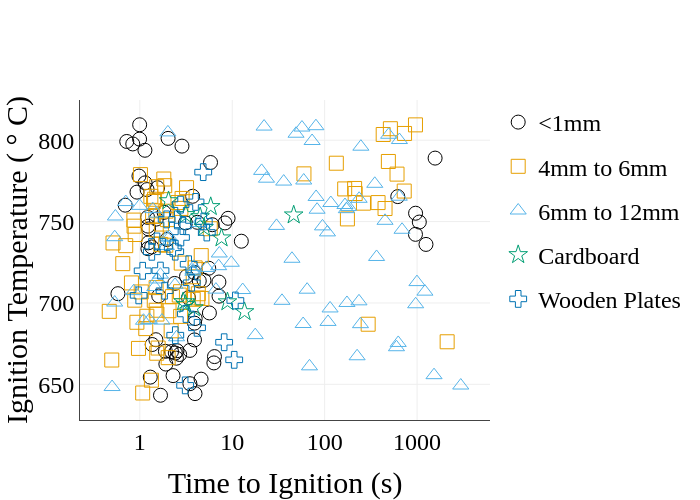
\includegraphics[width=\figureWidthSet]{Figures/ignition_comparison.png}
            \caption{Time to ignition and heater temperature at ignition for all fuel bed materials. 
            The dashed and dotted boxes emphasize the two general times-scales associated with ignition.}
            \label{fig:ignTime}
        \end{figure}
    

        \begin{figure}[htpb]
            \centering
                \begin{tikzpicture}
                \node[anchor=south west,inner sep=0] (image) at (0,0) {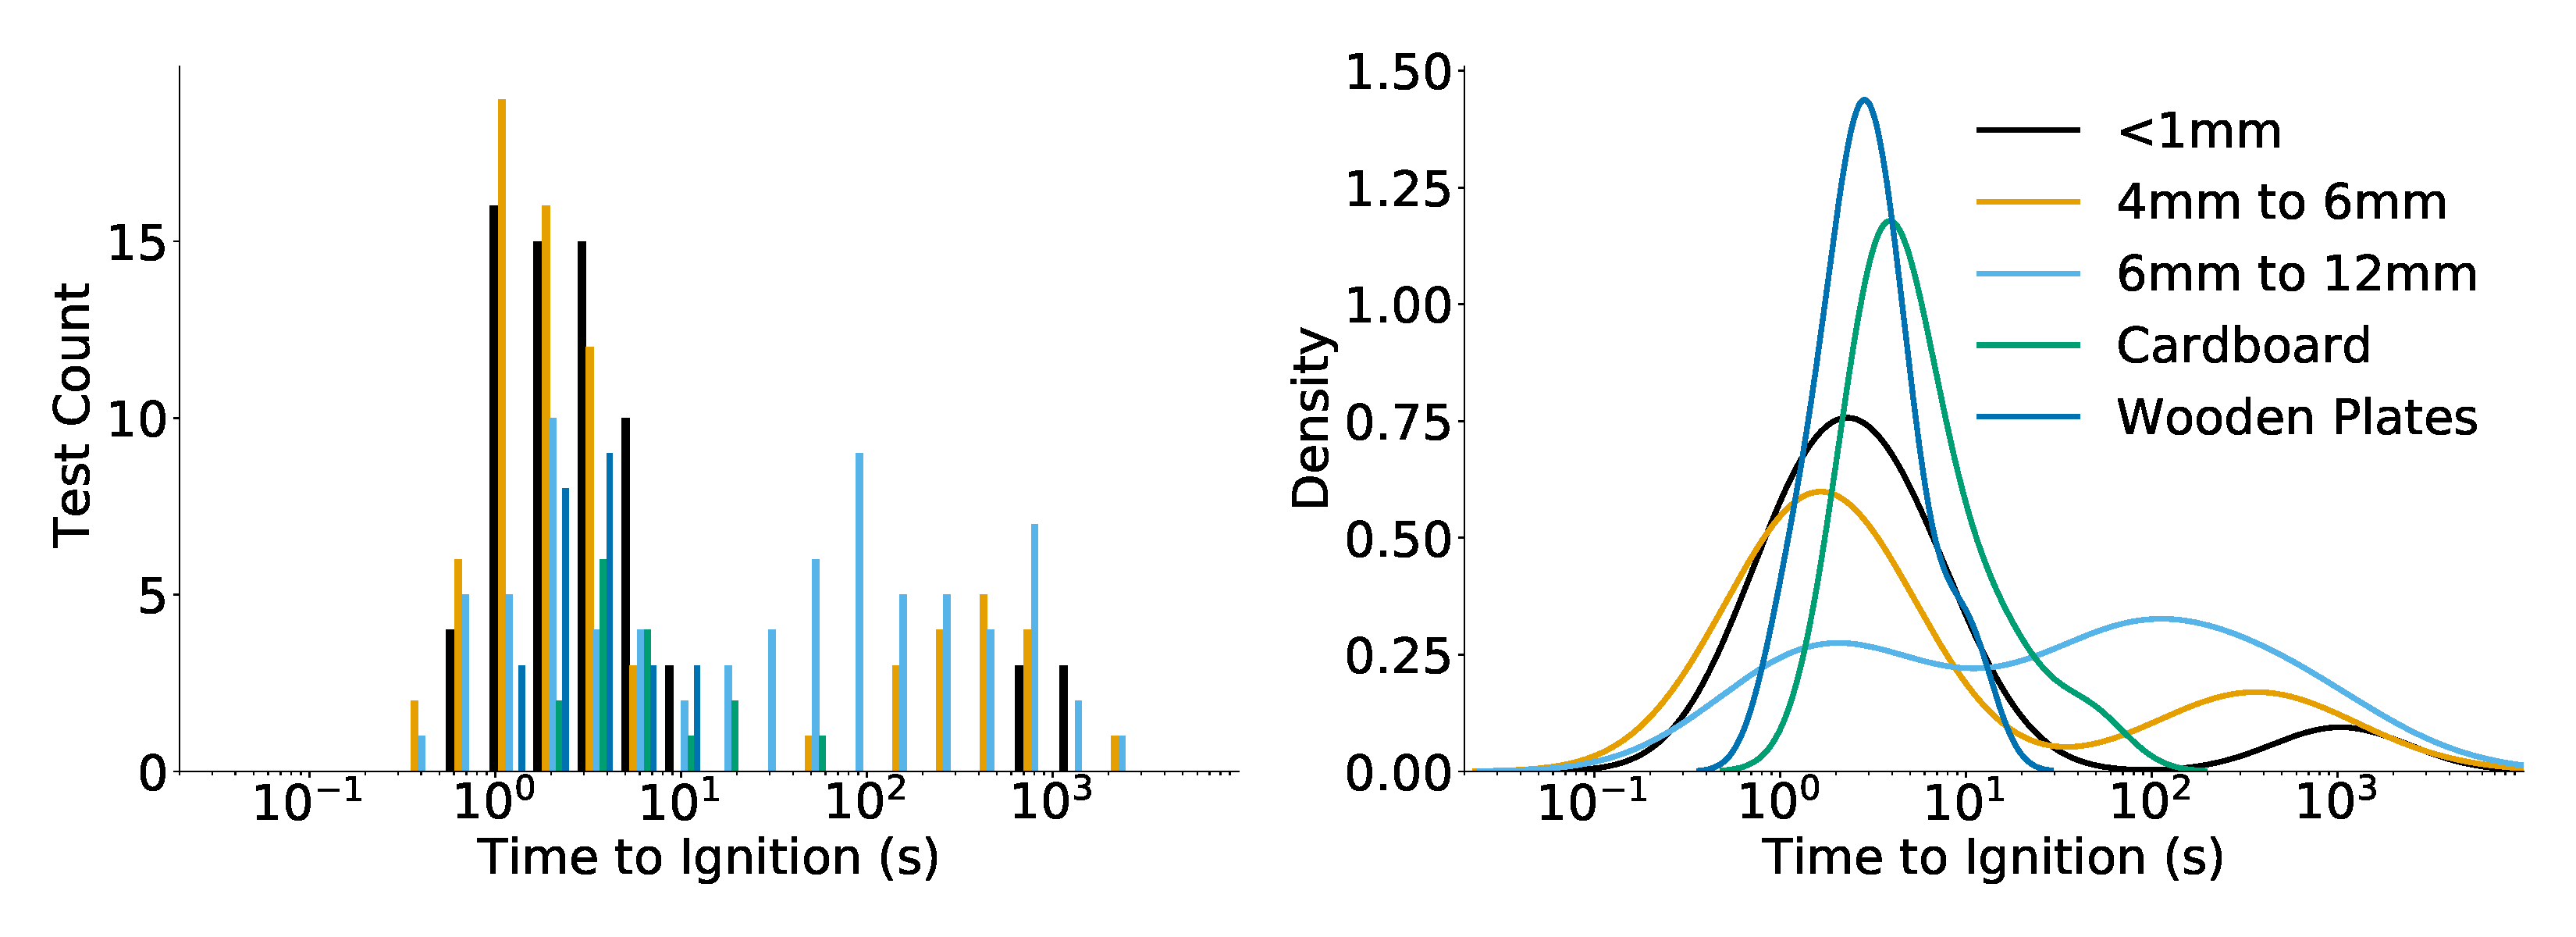
\includegraphics[width=\textwidth]{Figures/hist_and_kde.pdf}};
                    \begin{scope}[x={(image.south east)},y={(image.north west)}]
                        \draw[dashed, thick,rounded corners] (0.15, 0.185) rectangle (0.263, 0.9);
                        \draw[dotted, thick,rounded corners] (0.335, 0.185) rectangle (0.45, 0.52);
                        \draw[dashed, thick,rounded corners] (0.62, 0.185) rectangle (0.76, 0.9);
                        \draw[dotted, thick,rounded corners] (0.835, 0.185) rectangle (0.95, 0.52);
                    \end{scope}
            \end{tikzpicture}
            \caption{Ignition count (left) and probability density (right) of time to ignition for the fuel bed materials tested. The dashed and dotted boxes corresponding to the two zones of ignition from Figure~\ref{fig:ignTime}.}
            \label{fig:ignHist}
        \end{figure}
        
    The clustering of ignition times in either the $t_{ign} <$ 10\si{\second} or 100\si{\second}  $<t_{ign}<$ 1000\si{\second} time-scales is attributed to shifting of dominant heat transfer modes from conduction to radiation.  This shift occurs because of the heater fixture apparatus and the physical properties of the fuel beds. Initially, the heater and the fuel bed are in contact. The beds with larger particles have lower bulk densities; larger fractions of the fuel bed consist of air and have less contact area between particles. As a result, the effective thermal conductivity of the fuel beds decreases as the particle size increases as is shown in Table~\ref{tab:k_values}. For a fixed heater temperature the higher effective thermal conductivity for the smaller particles would result in a higher mass of particles above the pyrolysis temperature (as supported by calculations) producing conditions more conducive to ignition. As particle sizes decrease the pyrolysis products are also in closer proximity to the heater increasing the chances of either heating or piloted ignition as the gas flows over the heater. As a result, a larger percentage of smaller particle fuel beds ignite within 10\si{\second}, than the larger particle fuel beds (i.e., the second trend noted for Figure~\ref{fig:ignTime}). As heating progresses, a separation between the fuel bed and heater occurred because the heater was held in a fixed location while the fuel bed height decreased because of pyrolysis. Anecdotally this separation was observed to occur after $\approx$10\si{\second} for the various fuel beds. This separation causes the dominant mode of heat transfer to shift from conduction to infrared radiation. This change is significant because it corresponds to  ignition times to shifting from being less than 10\si{\second} to being generally greater than 100\si{\second}, as shown in Figure~\ref{fig:ignHist}. In addition, the larger particles tended to be longer thin particles which, on average, have a larger view factor per volume than the smaller particles. Hence, higher energy deposition per volume occurs for the larger particles when radiation is the dominant mode of heat transfer. As a result, the larger particle fuel beds more readily receive radiation and more readily ignite for $t_{ign} >$100\si{\second}, consistent with the trends discussed previously. The shift in dominant modes of heat transfer also causes solid plate fuel beds to not ignite after 100\si{\second}.  As separation between the heater and fuel occurs and heat transfer shifts to being dominated by radiation, the higher thermal conductivity of the solid materials (i.e., $k_{solid}=0.12$\si{\watt\per\meter\per\kelvin} vs $k_{<1mm} \approx 0.042$ \si{\watt\per\meter\per\kelvin}) reduces the temperature gradients, peak temperatures, and the release of pyrolyzates. 
    
    Further analysis of the time to ignition results reaffirm the influence of the fuel bed properties and heat transfer between the heater and fuel bed. A random forest regression model was implemented using the scikit-learn python package~\cite{scikit-learn} to identify which parameters were most correlated to the incidence of ignition occurring at either less than or greater than 10\si{\second}. The random forest regression model builds a series of independent decision trees based on experimental variables (e.g., average heat flux, particle size, etc.) and determines from those trees which variables have the largest influence on predicting the correct outcome (i.e., flaming ignition). A model is then assembled based on the specific values of each variable that best predict the desired outcome. Of the parameters recorded or calculated from experimental results, the incidence of ignition within each of the time scales was predicted with at least a 90\% certainty (out of bag and R$^{2}$ validation) when considering the estimated heat flux to the fuel bed, the fuel bed density, the power delivered to the heater at the time of heater contact, and the heater temperature. The power delivered to the heater at the time of heater contact is included as it serves as a comparison for a an initial reference of heat flux by which a comparison between ignitions that occurred in the radiation dominated mode at extended times which may bias the average heat flux values. The importance of these factors highlight the dependencies previously discussed in that the fuel bed properties and heat transfer to the fuel bed significantly influence the time-scales associated with ignition.  Moreover, the random forest analysis highlights a potential way that ignition may be predicted with a subset of information about the fuel bed. 
    
   The results and analysis just described focus on the characteristics of igniting cases; Figure~\ref{fig:ignProb} shows the probability of ignition for each of the fuel bed materials as a function of the heater temperature. The probability reported for each condition is based on the experiments being repeated at least five times.  In general, the ignition probability increased as the heater temperature increased, as expected because of the higher energy deposition. It is noted that as the heater temperature increases the potential for piloted ignition of pyrolysis gases increases. However, ignition occurs both above and below the piloted ignition temperature region and there is not a significant shift in trends at higher heater temperatures. This suggests that the influence of piloted ignition on the results is less significant than the increase of heat transfer rates to the fuel beds at higher temperatures. 
   
   When considering differences in ignition between fuel bed types the fuel beds with smaller particles typically had higher ignition probabilities at a temperature than beds with larger particles. At the lower temperatures, the plates tended to have lower ignition probabilities than the porous beds, but the plates transitioned from no ignition to unity ignition probability across a narrower range of temperatures than the porous fuel beds. It is noted that significant deviations from the overall trends (i.e., decreases in ignition probability) are apparent for the $L_{c}<$ 1\si{\milli\meter} particles at 675\si{\celsius} and 750\si{\celsius} and for the 6\si{\milli\meter} $<L_{c}<$ 12\si{\milli\meter} particles at 700\si{\celsius}. The cause of these deviations are unclear, but it is plausible the changes are caused by differences in ablation of the fuels and shifts in the dominant mode of heat transfer depending on the temperature.
        \begin{figure}[htpb]
            \centering
            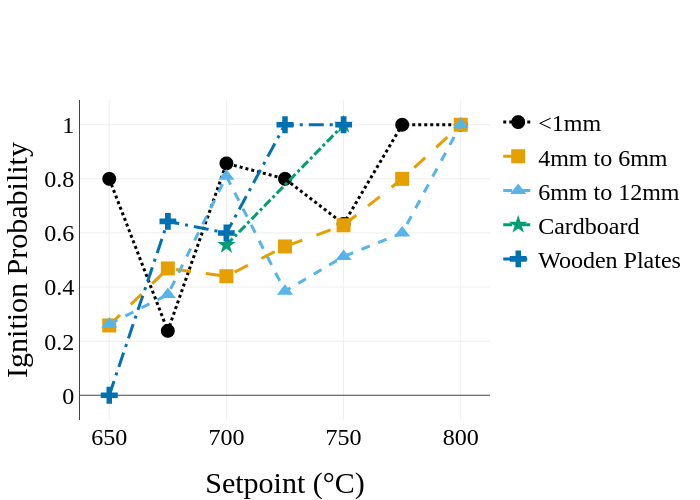
\includegraphics[width=\figureWidthSet]{Figures/setpoint_n5.png}
            \caption{Probability of ignition for each material as a function of heater set point temperature}
            \label{fig:ignProb}
        \end{figure}
    The sensitivities in ignition probability to the fuel bed characteristics, as shown in Figure~\ref{fig:ignProb}, are attributed to changes in area of the fuel bed in contact with the heater. Recall that the samples typically ignite within the first 10\si{\second}; hence conduction and the area of the fuel in contact with the heater are important in causing pyrolysis. As the particle size of the fuel bed increases fewer particles come into contact with the the heater, reducing the overall contact area. Additionally, the average distance between the heater and particles not in contact with the heater increases as particle size increases due to the reduced packing density of the particles. This may result in heat transfer from infrared radiation occurring over a more distributed volume within the fuel bed. As particle sizes increase the reduction in contact area and more distributed heat flux from radiation likely decrease the temperature gradient in the fuel bed as well as the local heat flux rates immediately adjacent to the heater, ultimately resulting in lower ignition probabilities for a fixed temperature as the particle size increases. 
    
    
    With regards to ignition of the Douglas-fir plates, it is expected that the solid materials behave similarly to the fuel beds with large particles (i.e., lower ignition probabilities at the lower temperatures) because the contact area between Douglas-fir plates and the cylindrical heater are more likely to be similar to the 6mm $<L_{c}<$ 12mm particles than the $L_{c}<$ 1mm particles. The Douglas-fir plates also have a much higher thermal conductivity and thermal mass than the particle fuel beds which is anticipated to result in similar temperature gradients between the largest particles and the plates. For the large particles infrared radiation to particles at greater distances from the heater, which would be occluded in the smaller particles, may act similarly to an increase in thermal conductivity and thus the similarity in ignition between the largest particles and Douglas-fir plates. The sharper transition from zero to unity ignition probability for the Douglas-fir plates is attributed to more consistent contact area between the heater and the plates from test to test. This uniformity is indicated in the narrower distribution of ignition times with only a $\approx$ 44\si{\second} difference between the shortest and longest ignition times for the Douglas-fir plates compared to $\approx$ 1550\si{\second} for the $L_{c}<$1mm particles. The narrower transition from non-ignition to ignition and the more consistent times to ignition of the Douglas-fir plates when compared to the particle fuel beds suggest that consistency in material properties and contact area between the heater and the fuel have a significant influence on ignition. 
    
    Similar to the time to ignition results, a random forest model was generated to gain insights into which parameters that are measured or derived are the most predictive of the occurrence of ignition of a fuel bed. The estimated heat flux to the fuel bed was the most influential parameter.  With the addition of the fuel bed density, heater temperature, and heat flux at contact with the fuel bed the prediction accuracy for ignition was 80\%.  These values were achieved based a 50\% test-train split of the entire dataset with out-of-bag and R$^{2}$ validation tests to measure predictive capabilities. The most noteworthy insight from this model is that the estimated average heat flux to the bed over the test duration has a much higher importance than the heater temperature for both porous and solid fuel beds. This is significant since the heat flux values, both upon contact and the overall average, encapsulate the effects of the heat transfer mode to the fuel bed unlike the surface temperature of the heater (or firebrand). A similar sensitivity of heat transferred to the fuel bed influencing ignition was observed by Fernandez-Pello et al.\cite{Fernandez-Pello2015}.
    
    Figure~\ref{fig:flux_comparison} shows the derived average heat fluxes to the fuel bed for each of the materials and heater temperatures tested. Results for igniting cases are represented by solid lines and non-igniting cases are represented with dashed lines. All the materials show two common trends except for cardboard plates, where not enough temperatures were evaluated to determine a trend. First, for tests where ignition occurred, and the heater setpoint was less than or equal to 750\si{\celsius} the heat flux to the fuel bed was higher than tests where ignition did not occur. Recall that the heater temperature is held constant, therefore variations in heat flux represent variations of heat transfer to the fuel. The implications of this are discussed in more detail later. Second, the heat flux values for tests where ignition occurred showed notable decreases in value for temperatures above 750\si{\celsius}, dropping lower than the values for the tests where ignition was not observed, in some cases.
        \begin{figure}[hbpt]
            \centering
            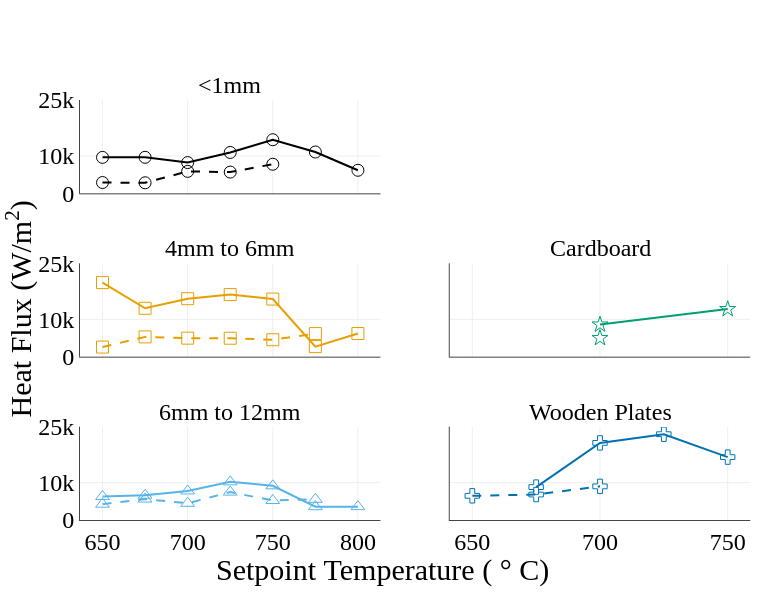
\includegraphics[width=\figureWidthSet]{Figures/power_comparison_trimmed.png}
            \caption{Comparison of estimated heat flux to the fuel bed for each material: dashed lines represents the mean of non-ignition tests and solid lines represent the mean of ignition tests for each heater temperature.}
            \label{fig:flux_comparison}
        \end{figure}
     Higher heat fluxes for the igniting cases compared to the non-igniting cases for the porous fuel beds are attributed to stochastic differences in contact area between the heater and the fuel bed particles. Seemingly, the tests with particles oriented in a manner that facilitates greater contact area have a higher heat flux due to increased conduction and are more likely to ignite. However, this assumption breaks down for high heater temperatures. At high heater temperatures (e.g., \textgreater750\si{\celsius}) the amount of heat transferred through infrared radiation appears be sufficient to counter differences in contact area and resulting conduction. Hence, this causes the reduction in the differences between igniting and non-igniting heat fluxes at the higher temperatures.  A sensitivity to the difference between igniting and non-igniting heat fluxes is noted depending on the particle sizes.  Specifically, in Figure~\ref{fig:flux_comparison}, the 4\si{\milli\meter} $<L_{c}<$ 6\si{\milli\meter} particles have greater differences in heat flux between the ignition and non-ignition cases when compared to the 6\si{\milli\meter} $<L_{c}<$ 12\si{\milli\meter} and $L_{c}$\textless1mm particles. The difference between igniting and non-igniting heat fluxes is correlated to the relative size of the particles compared to the diameter of the heater. For particles much smaller than the heater (\textless1\si{\milli\meter}) the random orientation of the particles would matter less than particles of similar size (4\si{\milli\meter} $<L_{c}<$ 6\si{\milli\meter}) as the heater. A similar phenomena is anticipated for particles larger than the heater (6\si{\milli\meter} $<L_{c}<$ 12\si{\milli\meter}), however, for the larger particles infrared radiation is anticipated to be more influential than conduction. Changes in contact between the heater and the fuel bed would then have a smaller effect on the rate of heat transfer as is shown by the spread in heat flux between ignition and non-ignition cases for the 6\si{\milli\meter} $<L_{c}<$ 12\si{\milli\meter} particles in Figure~\ref{fig:flux_comparison}. The 4\si{\milli\meter} $<L_{c}<$ 6\si{\milli\meter} particles appear to represent a near critical case where the conduction is still the driving heat transfer mode but variation in contact area is high producing a larger spread in heat flux.
     For the wooden plates a smaller number of heater temperatures with both ignition and non ignition heat flux values is observed suggesting test to test variation in contact area is not significant enough to prevent ignition.

    Results from OpenFOAM simulations of temperature profiles provide further insights into the effects of varying heat flux on ignition. Figure~\ref{fig:volumes} shows regions of the fuel bed above the pyrolysis temperature for (row I) a fixed 750\si{\celsius} boundary condition, (row II) a heat flux boundary condition based on the average values from ignition tests at the 750\si{\celsius}, and (row III) a heat flux boundary conditions based on  average heat fluxes for non-ignition tests at the 750\si{\celsius}. Column A shows the results for the fuel bed with $L_{c}<$ 1mm, column B with a bed of 4mm $<L_{c}<$ 6mm, and column C with a bed of 6\si{\milli\meter} $<L_{c}<$ 12\si{\milli\meter} particles. For the constant temperature boundary shown in row I, the region of the fuel bed above the pyrolysis temperature increases as particle sizes increase from left to right. Note, however, that the mass of the fuel bed material above the pyrolysis temperature decreases from left to right due to the decreasing density and thermal conductivity of the fuel bed as particle sizes increases. Specifically, the estimated mass of the fuel bed above the temperature for the onset of pyrolysis is 2.79\si{\micro\gram}, 1.59\si{\micro\gram}, and 1.55\si{\micro\gram} for columns (A), (B), and (C), respectively.  As a result, it is expected that the fuel bed with the smallest particles would release the most pyrolzates. 
    
    Perhaps surprising, is the difference in area at elevated temperatures between columns A and B in row II. Recall from Figure~\ref{fig:ignProb} that at this heater temperature (750\si{\celsius}) the particles with $L_{c}<$ 1\si{\milli\meter} (i.e., column A), and the 4\si{\milli\meter} $<L_{c}<$ 6\si{\milli\meter} (i.e., column B) have nearly identical ignition probabilities; however, the calculated average temperatures and region undergoing pyrolysis are notably different (e.g., 175\si{\celsius}).  More importantly, a 30\% mass increase in pyrolyzates occurs from $L_{c}<$ 1\si{\milli\meter} to 4\si{\milli\meter} $<L_{c}<$ 6\si{\milli\meter} conditions.  The corresponding ignition delay time, calculated using mass of pyrolyzates released and the average temperature of the pyrolysis region, was 0.5\si{\second} for the $L_{c}<$1\si{\milli\meter} gaseous products compared to 0.06\si{\second} for the 4\si{\milli\meter} $<L_{c}<$ 6\si{\milli\meter} products. The differences in ignition delay time results from differences in the average fuel bed temperature and in the global equivalence ratio as pyrolyzates are released. Physically, these ignition delay times correspond to the characteristics of the pyrolyzates exiting the fuel bed. The differences in ignition delay time would suggest that the particles with 4\si{\milli\meter} $<L_{c}<$ 6\si{\milli\meter} would ignite more readily, counter to the measured similar ignition probability.  Note, however, that the calculated velocity of the gaseous products also varies, specifically 4.3$\cdot10^{-3}$\si{\meter\per\second} for the $L_{c}<$1\si{\milli\meter} fuel compared to 2.6$\cdot10^{-2}$\si{\meter\per\second} for the 4\si{\milli\meter} $<L_{c}<$ 6\si{\milli\meter} fuel bed.  In short, consideration of both the ignition delay time and exit velocity of the gases maybe needed to more completely capture ignition probabilities.

    The Damkohler number (\textit{Da}), which represents the ratio of the transport to chemical times-scales, has been used previously to consider ignition behavior~\cite{Dai2013}, and is now considered to help evaluate ignition behavior.  In this work, the ratio of the heater diameter $D$ normalized by the product of the exit velocity ($V_{exit}$) and ignition delay time ($\tau$) were considered, to create a Damkohler number of ignition for porous beds. This analysis results in the non-dimensional values of 2.42, 4.04, and 7.66 for the smallest to largest particles (respectively) for the results just described in the previous paragraph. Note that the smaller the (\textit{Da}) the smaller the transport time (relative to chemical time-scale) and the less time that a parcel of reactants is near the high temperatures of the heater. In its limit, rectants may diffuse/advect away from the fuel prior to ignition.
        \begin{figure}[htpb]
            \centering
                \begin{tikzpicture}
                \begin{scope}[xscale=-1, yscale=1]
                    \node[anchor=south west,inner sep=0] (image) at (0,0) {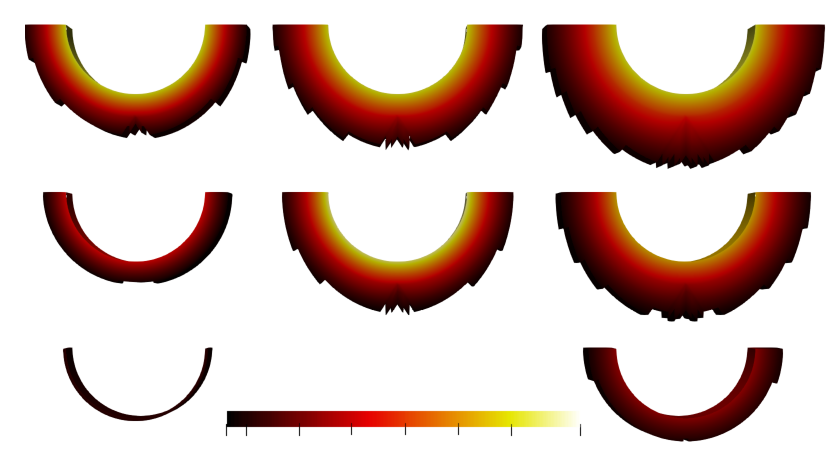
\includegraphics[width=\figureWidthSet]{Figures/fuel_bed_temperature_comparison_colorbar.png}};
                \end{scope}

                    \begin{scope}[x={(image.south east)},y={(image.north west)}]
                        \node at (-0.1, .82) {I};
                        \node at (-0.1, .5) {II};
                        \node at (-0.1, .15) {III};
                        \node at (0.16, -0.1) {A};
                        \node at (0.5, -0.1)  {B};
                        \node at (0.835, -0.1) {C};
                        \draw[dotted] (0, 0.64) -- (0.985, 0.64);
                        \draw[dotted] (0, 0.305) -- (0.985, .305);
                        \draw[dotted] (0, 0.045) -- (0.985, 0.045);
                        \draw[dotted] (0.30, 0.045) -- (0.30, 1);
                        \draw[dotted] (0.625, 0.045) -- (0.625, 1);
                        \draw[dotted] (0.985, 0.045) -- (0.985, 1);
                        \node at (0.27, 0.0) {220 (\si{\celsius})};
                        \node at (0.7, 0.0) {750 (\si{\celsius})};
                    \end{scope}
            \end{tikzpicture}
            \caption{Calculated region of fuel bed above the pyrolysis temperature 10\si{\second} after heater contact for a fixed  750\si{\celsius} boundary (I), ignition event heat flux (II), and non-ignition test event flux (III) for $L_{c}<$ 1mm (A), 4mm $<L_{c}<$ 6mm (B), and 6mm $<L_{c}<$ 12mm particles (C).}
            \label{fig:volumes}
        \end{figure}
    
    To further explore the potential role of using a (\textit{Da}) to characterize ignition propensity or porous, Figure~\ref{fig:nonDimPlot} shows the (\textit{Da}) number for the gaseous products at the exit of the fuel bed for each particle size and heater set point. Data from the plates is excluded, as the supporting calculations were beyond the scope of the work.  The abscissa is plotted relative to the average heat flux to the fuel bed multiplied by the thermal diffusivity of the fuel bed. These values were selected to include the influence of heat flux and thermal properties of the fuel beds in the characterization of ignition. Effectively, the chemical properties of the fuel bed and transport behavior are captured in the \textit{Da} analysis and thermal properties are included in the heat flux and thermal diffusivity. The lower right area of the plot, labelled No Ignition, represents values estimated to be less conducive to ignition (i.e., longer ignition delay times) than those observed to produce ignition in experiments. The region where ignition is expected contains the remainder of the plot and represents values estimated to equally or more conducive to ignition (i.e., higher heat fluxes and shorter ignition delay times) than those observed in experiments. The relative similarity trends in ignition behavior when considering the (\textit{Da}) indicate that considering the local transport conditions may be important to predicting ignition, in addition to considering the local heat flux and release of pyrolyzates. 
        
        \begin{figure}
            \centering
                            \begin{tikzpicture}
                \begin{scope}[xscale=-1, yscale=1]
                    \node[anchor=south west,inner sep=0] (image) at (0,0) {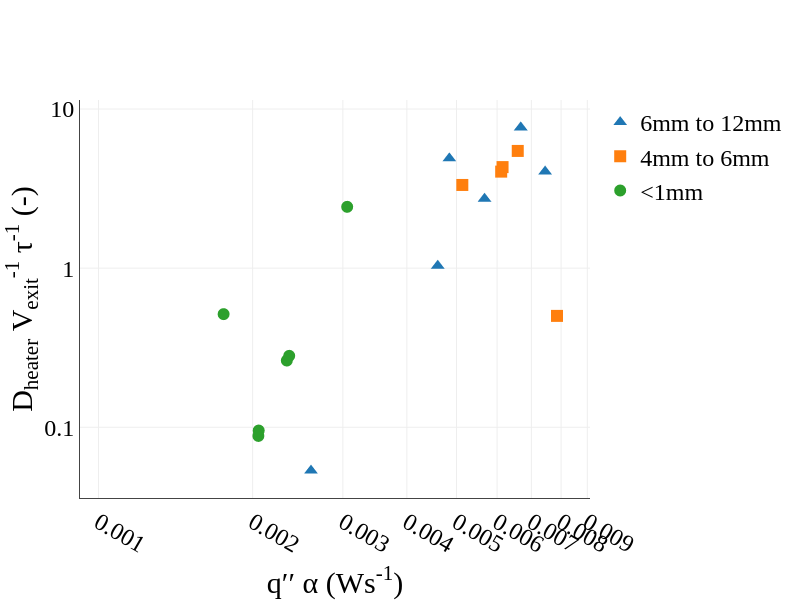
\includegraphics[width=\figureWidthSet]{Figures/ignition_trend.png}};
                \end{scope}

                    \begin{scope}[x={(image.south east)},y={(image.north west)}]
                        %   \fill[pattern=north east lines, pattern color=wongyellow, opacity=0.6] (0.1, 0.14) -- (0.73, 0.14) -- (0.73, .83) -- (0.6, 0.83) --cycle;
                         %\fill[pattern=north west lines, pattern color=wongorange, opacity=0.7] (0.40, 0.175) -- (0.73, 0.175) -- (0.73, .45) --(0.4, 0.45) --cycle;
                        \node at (0.567, 0.3) {No Ignition};
                    \end{scope}
            \end{tikzpicture}
            \caption{Comparison of non-dimensional chemical and flow timescale (for the igniting cases) as a function of heat flux time and thermal diffusivity. Conditions where ignition and non-ignition are anticipated are highlighted.}
            \label{fig:nonDimPlot}
        \end{figure}
    
    
   
\section{Summary and Conclusions}
    Flaming ignition tests have been conducted for porous Douglas-fir beds, Douglas-fir plates, and cardboard plates. A cylindrical cartridge heater was used as a firebrand surrogate. Heater temperature and electrical power to the heater were collected throughout each test. The derived heat flux to the fuel bed was within the range reported in literature of heat fluxes delivered by firebrands.  The time to ignition and probablity of ignition were used to evaluate the ignition propensity for the various fuel beds and heater temperatures.  A simplified heat transfer, pyrolysis, and ignition delay model was developed and used to provide further insights into the physical processes associated with ignition. The specific conclusions from this work are as follows.
        \begin{enumerate}
            \item 
                Smaller particles ignite more readily in porous beds than larger particles when heat transfer from the heater is primarily through conduction. This was evident by higher ignition probabilities, in general, of the smaller particles for a fixed heater temperature. As particle sizes increase radiant heat transfer becomes more important and fuel beds with larger particles were more likely than smaller particles to ignite at extended times (\textgreater 100\si{\second}) due to the increased importance of radiant ignition. 
            \item
                Douglas-fir plates ignite at times where conduction is the dominant mode of heat transfer (\textless 10\si{\second}) due to the higher thermal conductivity of the solid plates. The ignition probability of plates was the most similar to the larger particle, in particular at lower heater temperatures, due to dispersed heating of the porous fuel bed through radiation and the increased thermal conductivity of the plates creating similar temperature profiles. The rise in ignition probability  over a smaller heater temperature range time with temperature results from more consistent contact between the heater and plate surface.
            \item 
                Heat flux delivered to the fuel bed, when compared to heater temperature, is more indicative of ignition likelihood and ignition time for porous fuel beds. Heat flux is a more significant predictor of ignition because it captures differences in heat transfer modes and particle contact that heater temperature values do not. While this finding is not new, what is novel is that the mixed mode of heating (conduction and radiation) has a significant impact on the flaming ignition of fuel beds.
            \item 
                Consideration of the transport characteristics of pyrolyzate gases near the high temperature source can be important for more fully predicting ignition propensity. A \textit{Da} of ignition, in relation to the measured heat flux and thermal diffusivity of the fuel beds, is a promising relationship for predicting ignition for the porous fuel beds.  
        \end{enumerate}
    Further work is needed to verify that the \textit{Da} may be used to predict ignition for solid surfaces and for porous fuel beds with varying chemical compositions.  If proven valid, the (\textit{Da}), measured/predicted heat fluxes, and fuel bed properties may be used to help predict ignition of fuel beds both in and out of the WUI, ultimately helping to increase the effectiveness of fire prevention and suppression efforts.

%!TEX root = thesis.tex

\renewcommand{\TheTitle}{Influence of Wind on Flaming Ignition of Porous Wood Fuel Beds}
\renewcommand{\TheAuthors}{Derek Bean, David L. Blunck \\ \\ My contributions to this work included the design of the experiments, fabrication of the experimental apparatus, collecting data, data analysis, conducting modelling efforts, and preparation of the manuscript.}

\renewcommand{\TheAddress}{
\textbf{Status: Under Review} \\
\textit{Fire Safety Journal}
}

\PaperHeader{\chapter{\TheTitle}\label{chap:manuscript2}}{\TheAuthors}{\TheAddress}
\newpage
%\chapter{\TheTitle}

\section{Abstract}
\label{sec:abtract2}
    The increasing severity of wildfires and the expansion of the wildland urban interface has increased the need to better protect homes from fires. Ignition of fuels (e.g., needles, mulch, leaves) near or on homes by firebrands can be a significant risk factor for home loss. Understanding the environmental factors that control the ignition of fuel beds by firebrands is important to reducing the risk of home loss. This study evaluates the effect of the wind speed and direction on the probability of ignition of fuel beds by firebrands. The fuel beds, Douglas-fir particles between 1.3\si{\milli\meter} and 2.3\si{\milli\meter} in size, were ignited by a cartridge heater (i.e., surrogate firebrand). Flaming ignition probability and time to ignition were determined for three different wind speeds and three wind directions. CFD calculations were performed to provide additional insights into the flow field leading up to ignition. Increases in wind speed above quiescent conditions reduced the temperature required for flaming ignition. An increase in wind speed to 3.5\si{\meter\per\second} from quiescent increased the ignition probability of fuel beds from 60\% to roughly 100\% depending on the wind direction. However, a threshold was observed for some wind directions where a further increase of wind did not increase the ignition probability. Temperatures required for flaming ignition and the time to ignition were sensitive to the wind direction. Ignitions occurred at the lowest temperatures when the wind direction was perpendicular to the surrogate firebrand. High speed images of the ignition process and  corresponding CFD calculations indicate that ignition occurred in regions with long residence times. The sensitivity to wind direction is attributed to differences in recirculation zones which changes the residence time of pyrolyzates. 
    
\section{Introduction} 
\label{sec:introduction2}
    As the severity of wildfires and the number of homes in the wildland urban interface (WUI) increases the need is rising to better protect homes from wildfires~\cite{Marlon2012Long-termUSA, Manzello2013, Barrett2020}. A common way that homes are destroyed during wildfires is by the ignition of fuel beds (e.g., needles, leaves, or landscaping materials) by firebrands. Flames may then spread to and subsequently engulf the structure~\cite{Manzello2014, Maranghides2013NISTIgnitions}. A better understanding of how fuel beds ignite around homes is necessary in order to better protect homes from this phenomena. While the overall mechanisms by which ignition by firebrands occur are generally well understood, predicting when ignition will occur remains elusive~\cite{Fernandez-Pello2017}. One of the reasons for the limitations of predictive capabilities is the lack of quantification with respect to how changes in the fuel bed and environmental conditions influence the likelihood of ignition~\cite{Finney2013}.
    
    Wind is an environmental factor that can have a significant impact on the spread of fires. First, increases in wind speed increase the size of firebrands produced~\cite{Suzuki2013}, potentially leading to firebrands of higher energy content. Second, firebrand laden winds flowing around structures can lead to accumulation of firebrands in particular regions~\cite{Suzuki2020a, Manzello2014}. Third, the amount of heat imparted to a fuel bed by firebrands can increase as wind speeds increase~\cite{Hakes2019a, Tao2020, Salehizadeh2021}. 
    
    In many studies the presence of wind either increases the probability of ignition by firebrands~\cite{Filkov2016, Manzello2006, Manzello2006a, Matvienko2018, Ellis2015, Plucinski2008}, or facilitated ignitions that did not occur without wind~\cite{Ellis2011}. For example, in tests with natural fuel beds (e.g, needles, leaves, and grass) and firebrands (e.g., burning twigs, bark, and cones) increases in ignition probability were observed, in some instances, with increases in wind speeds and changes in wind direction~\cite{Ganteaume2009}. Similar increases in ignition probability as wind speed increases have been observed in fuel beds with hot metal particles as ignition sources~\cite{Wang2017}. Increases in ignition propensity have been postulated to be caused by greater oxygen availability and/or increased mixing as a result of the wind speed. 
    
    In the aforementioned studies the heat transfer rates from the firebrands to the fuel beds may have changed (likely increased due of faster reaction rates) due to the presence of wind. Changes in the heat transfer rate from the firebrands and changes in the flow field near the fuel bed make it challenging to fully identify cause(s) for wind increasing/altering ignition behavior.
    As a result it is not clear to what extend changes in ignition behavior are caused by the interaction of the fuel bed with the wind or changes in heat transfer from the firebrands.
    It is important to decouple these two effects to better understand how each factor impacts ignition. A better understanding of ignition sensitivities to wind can ultimately be used to better design building codes and standards to protect structures near the WUI.

    
    
    %A similar increase in ignition propensity in the presence of wind has been observed for fuel beds in contact with hot metal particles, in contrast to firebrands~\cite{Wang2017}. This observations suggests that a sensitivity to oxygen availability caused by wind over the fuel bed independent from the effects of heat transfer from firebrands due to wind. Ultimately, the magnitude of the impact that increasing mixing and oxygen availability has on ignition of fuel beds has not been isolated or characterized with respect to wildland fire applications. Such knowledge can be used to ensure that models and/or test standards capture the required physics.
    
    %Fortunately, a framework for considering the relative effects of mixing and oxygen availability exists. This relationship is the Damkohler number (Da)\cite{Law2006CombustionPhysics}. The Da is typically used to predict ignition of gaseous fuel-oxidizer mixtures relative to the ratio the the fluid dynamic residence time and the time for chemical reactions to occur. 
    
    With this background and motivation, the objective of this study is to quantify how changing environmental factors, specifically wind speed and direction, influences ignition of a fuel bed in contact with a firebrand. It is expected that the results of this work will help further the understanding of the influence of wind on fuel bed ignition and may allow for better protection of structures in the WUI.

\section{Methodology}
\label{sec:methods2}
    \subsection{Experimental}
    The probability of flaming ignition for beds of Douglas-fir particles were measured for three different wind speeds and firebrand orientations in a wind tunnel. Douglas-fir particles serve as a surrogate for natural fuels near the WUI. Figure~\ref{fig:windTunnelApparatus} shows a representation of the wind tunnel, fuel bed, and the portion of the device for lowing a cartridge heater (i.e., surrogate firebrand) onto the fuel bed.  The wind speeds tested were 0.5 \si{\meter\per\second}, 3.5 \si{\meter\per\second}, and 5.8 \si{\meter\per\second}. Higher wind speeds were not tested to avoid material from the fuel bed blowing away. The wind speed was measured with a TSI-IFA300 hot wire probe. Tests were conducted with the heater placed parallel, perpendicular, and 45\si{\degree} relative to the wind direction for each wind speed. 

    
    The fuel beds were created in a multi-step process. Kiln dried Douglas-fir lumber was planed, then granulated, and finally screened such that the particles fit through a 2.3\si{\milli\meter} screen but not a 1.3\si{\milli\meter} screen. The fuel was placed in a 140\si{\milli\meter} diameter glass container with a depth of 70\si{\milli\meter} before insertion into the wind tunnel. The average bulk density of the fuel beds was 74.2\si{\kilo\gram\per\cubic\meter}.   
    
    A minimum of 20 ignition tests were conducted for each experimental condition with a total of 241 tests.  The temperature set points of the heater for the various experiments were identified using the three-phase optimal design procedure~\cite{Wu2014, Burke2017TestPractice}. The three-phase optimal design is a sequential procedure used to ascertain the probability of a binary outcome (i.e., ignition or non-ignition) with a limited number of tests. The logistic regressions and 95\% confidence intervals of the ignition probability were calculated using the scikit-learn python package~\cite{scikit-learn}. A fuel bed was considered to ignite if a flame was observed and persisted after the heater was removed. If flaming ignition was not observed after 3000\si{\second} of heater contact the heater was removed and the test was considered to have a no-ignition outcome.
     \begin{figure}[hbpt]
            \centering
            \resizebox{0.5\columnwidth}{!}{%
                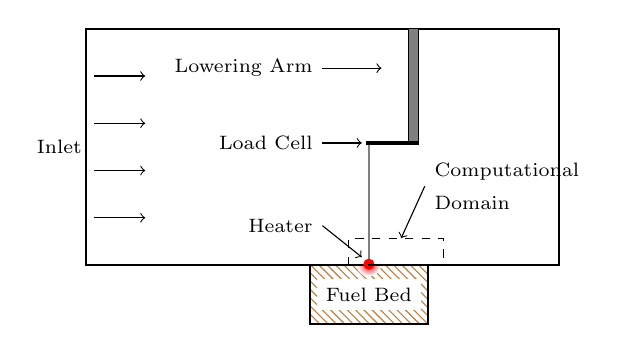
\begin{tikzpicture}
                    \filldraw[pattern=north west lines, pattern color=brown, thick] (2.84, 0)  rectangle (4.34, -.75) node[pos=0.5,rectangle,fill=white] {\scriptsize Fuel Bed};
                    \fill [draw=white,  inner color=red, outer color=white ] (3.59, 0.01) circle (0.15);
                    \filldraw[draw=black,fill=white, thick] (0, 0)      rectangle (6, 3);
                    \fill[fill=black!50] (3.58, 0) rectangle (3.61, 1.52);
                    \fill[fill=black] (3.55, 1.52) rectangle (4.23, 1.57);
                    \filldraw[draw=black, fill=black!50] (4.09, 1.57) rectangle (4.22, 3);
                    \fill[draw=red, fill=red] (3.59, 0.01) circle (0.0635);
                    \draw [<-] (3.5, 0.1) -- (3, 0.5) node[left] {\scriptsize Heater};
                    \draw [<-] (3.5, 1.55) -- (3, 1.55) node[left] {\scriptsize Load Cell};
                    \draw [<-] (3.75, 2.5) -- (3, 2.5) node[left] {\scriptsize Lowering Arm};
                    \draw[->]         (0.1, 0.6) -- (0.75, 0.6);
                    \draw[->]         (0.1, 1.2) -- (0.75, 1.2);
                    \node[right] at (-0.75, 1.5) {\scriptsize Inlet};
                    \draw[->]         (0.1, 1.8) -- (0.75, 1.8);
                    \draw[->]         (0.1, 2.4) -- (0.75, 2.4);
                    \draw[draw=black, dashed] (3.336, 0) rectangle (4.54, 0.34);
                    \draw[->]         (4.3, 1) -- (4.0, 0.34);
                    \node[right, align=left] at (4.3, 1) {\scriptsize Computational\\ \scriptsize Domain};
                \end{tikzpicture}
                }
            \caption{Diagram of the experimental wind tunnel apparatus. Air flows through the wind tunnel from left to right. The dashed region represents the domain subset used for computational efforts.}
            \label{fig:windTunnelApparatus}
        \end{figure}
    
    The energy imparted to the fuel bed was estimated by applying an energy balance to the heater. Typical heat fluxes to the fuel bed ranged from 5\si{\kilo\watt\per\square\meter} to 50\si{\kilo\watt\per\square\meter}. Similar values have been reported for studies of heat fluxes from firebrands~\cite{Hakes2019a, Tao2020}. The power delivered to the heater was measured using a CR9580-10 current sensor and a ZMPT101B voltage sensor. Temperature distributions, created from infrared images of the heater taken with a FLIR SC6700 camera, were used to estimate heat loss to the ambient. A black body calibration was performed to correlate photon counts from the camera to temperature and produce a longitudinal temperature distribution. The circumferential temperature of the heater was considered uniform.
    
    High speed images of the ignition process were captured using a Phantom VEO 710 camera for select conditions. The images were used to provide insights into differences between ignition processes. Images were collected at 5\si{\kilo\hertz}. 
    
    \subsection{Computational}
    
    A simplified computational model was implemented to provide further insights into the processes leading up to ignition for the different configurations. Fluid flow around the heater, heat transfer from the heater to the fluid, and the release of pyrolysis gases into the fluid domain were simulated for the 5.8\si{\meter\per\second} wind speed and the three heater orientations. Simulations were conducted in two parts. First the average mass flux and average thermal properties of pyrolyzates were estimated. These estimations were conducted through a non-reacting heat transfer model to the fuel bed to obtain an estimate for the mass of fuel bed material above the pyrolysis temperature of 220\si{\celsius}. The thermal properties of the fuel bed were estimated using correlations for porous media~\cite{bergman2011fundamentals} and the average bulk density of the fuel beds during the tests. The heat transfer to the fuel bed was determined from the energy balance for a heater temperature corresponding to the 50\% ignition probability. 
    
     The temperature evolution of the fuel bed over time was used to estimate the pyrolysis products. The calculations solved the heat diffusion equation (Equation~\ref{eqn:heatDiffusion} to observe the spatial and temporal evolution of the fuel bed temperatures. Calculations were conducted for 10 seconds for two reasons. First, the assumptions, that are outlined in the following section, reduce the accuracy of the model due to pyrolysis of the fuel bed in the experiment changing the fuel bed properties. Second, in absence of changes in fuel beds due to pyrolysis a simulation time of ten seconds provided sufficient insight into trends observed in the experiments. 
        \begin{equation}
            \frac{\partial \left(\rho h \right)}{\partial t} = \frac{\partial}{\partial x_{j}} \left( \alpha \frac{\partial h}{\partial x_{j}} \right)
            \label{eqn:heatDiffusion}
        \end{equation}
     The assumptions for the temperature modeling of the fuel bed are as follows:
        \begin{itemize}
            \item Fuel beds were considered to be non reacting. 
            \item Thermal properties of the fuel bed were considered independent of temperature.
            \item The temperature evolution of the fuel bed is symmetric around the centerline of the heater.
            \item The heat losses to the ambient are significantly less than the heat transfer from the heater. Thus, the interface between the fuel bed and air was considered insulated.
            \item The fuel bed was modeled as a solid with the thermal and physical properties either measured or derived from experimental measurements.
        \end{itemize}

    
    The mass of pyrolysis gases released was then estimated using 0D calculations in Cantera. The chemical composition of the fuel bed was estimated from the Bioengineering Feedstock Library database~\cite{feedstock}. The BioPox mechanism~\cite{Dhahak2019} was used for pyrolysis kinetics in the fuel bed. Species were considered to be released into the flow domain if they existed in the gas phase biomass mechanism Bio1412~\cite{Ranzi2008}. More detail for the species selection process is available in previous work~\cite{Bean2021}. The Cantera calculations considered the fuel bed material as an insulated fixed mass reactor. The following equations were solved to obtain the temperature and species concentrations of the pyrolyis products. 
        \begin{equation}
            \pder[m]{t} = 0
        \end{equation}
        
        \begin{equation}
            m \pder[\left( m Y_k \right)]{t} = \dot{m}_{k, gen} = V \dot{\omega}_k MW_k
        \end{equation}
        \begin{equation}
            mc_{v} \pder[T]{t} = \dot{Q} - \sum_{k} \dot{m}_{k,gen}u_k
        \end{equation}
    Where $Y_k$, $\dot{m}_{k}$, and  $\dot{\omega}_k$ are the mass fraction, mass generation rate, and generation rate of each species $k$ in the mechanism used. $V$ is the volume of the fuel bed material in the reactor. The species generation rates $ \dot{\omega}_k$ are determined from the reactions included in the mechanism. The mechanism used for pyrolysis contains four different types of chemical reactions. The equations used to calculate the reaction rates for an elementary reaction is:
        \begin{align}
            k_f &= AT^{b}e^{-E_a/RT}\\
            R_{f} &= [A][B]k_f 
        \end{align}
    Where $R_f$ is the forward reaction rate, $k_f$ the reaction rate constant, $E_a$ the activation energy, $b$ is the temperature exponent and $R$ is the gas constant. Similarly, the reaction rates for three body reactions are calculated as:
        \begin{align}
            R_f &= [A][B][M]k_f \\
            [M] &= \sum_{k}\epsilon_k C_k
        \end{align}
    Where $\epsilon_k$ and $C_k$ are the collision efficiency and concentration of each species, respectively. Fallof reaction rates are calculated using the reduced pressure $P$ defined as:
        \begin{equation}
            P = \frac{k_0[M]}{k_\infty}
        \end{equation}
    The reaction reaction rate is then calculated as:
        \begin{equation}
            k_f (T, P) = k_{\infty} \left( \frac{P}{1+P}\right) F(T,P)
        \end{equation}
      Pressure dependent P-Log reaction rates are calculated for intermediate values using a logarithmic interpolation between two reaction rates $k_1$ and $k_2$ at pressures $P_1$ and $P_2$ as:
        \begin{equation}
            \log k_f(T,P) = \log k_1(T) + (\log k_2(T) - \log k_1(T))\frac{\log P - \log P_1}{\log P_2 - \log P_1}
        \end{equation}
    The overall generation rate of each species ($\dot{\omega}_k$) is then defined as the sum of the individual reaction rates $R_f$ for all of the reactions where the species is present. 
        \begin{equation}
            \dot{\omega}_k = \sum_i^N \nu_i R_{f, i}
        \end{equation}
    Where $\nu_i$ number of each species produced for each reaction.
    
   The second step of the computational effort simulated pyrolysis gas distribution in near the heater using OpenFOAM~\cite{Foundation2020}. The mass, momentum, species, and energy equations for the OpenFOAM calculations are shown below.
            \begin{equation}
                \pder[p]{t} + \pder [\rho u_{j}] {x_{j}} = 0
            \end{equation}
            
            \begin{equation}
                \pder[\left( \rho Y_{k} \right)]{t}  + \pder[\left( \rho u_{j} Y_{k}\right)]{x_{j}}  = 
                \pder[\mu_{eff}]{x_{j}}  \pder[Y_{k}]{x_{j}} 
            \end{equation}
            
            \begin{equation}
                \pder[\left(\rho u_{i}\right)]{t}  + \pder[\left( \rho u_{rj}u_{i}\right)]{x_{j}}  + \rho \epsilon_{ijk}\omega_{i}u_{j}= - 
                \pder[p_{rgh}]{x_{i}}  - \pder[\left( \rho g_i x_j \right)] {x_i}  + \pder{x_j} \left( \tau_{ij} + \tau_{t_{ij}} \right)
            \end{equation}
            
            \begin{multline}
                \pder[\left(\rho h \right)]{t} + \pder[\left( \rho u_j h \right)]{x_j} + \pder[\left(  \rho k \right)]{t} + \pder[\left( \rho u_j k\right)]{x_j} = \\ -
                \pder[\left( q_i + q_{ti} \right)]{x_i} + \rho r + q_{rad} + \pder[p]{t} - \rho g_j u_j + \pder[\left( \tau_{ij} u_i \right)]{x_j}
            \end{multline}
      The computational domain used is outlined in Figure~\ref{fig:windTunnelApparatus} with a dashed rectangle. A subset of the wind tunnel test section near the heater(s) was considered for the simulation of the flow over the heater(s). For all three heater angles a constant cross section normal to the flow was used. The dimensions of the plane normal to the flow was 110\si{\milli\meter} wide and 48\si{\milli\meter} tall. The lengths of the domains varied to maintain a domain size of 5D upstream and 14D downstream of the heater. The domain lengths were 170\si{\milli\meter} for the 45\si{\degree} and parallel configurations and 120\si{\milli\meter} for the heater perpendicular to the flow. The number of cells for each domain were 420728, 424308, and 307252 for the parallel, 45\si{\degree}, and perpendicular cases. Cell sizes ranged from 0.1\si{\milli\meter} near the heater to 4\si{\milli\meter} in the bulk flow region in the center of the domain. 
      
      The inlet boundary conditions were determined from experimental measurements where the bulk wind speed was 5.8 \si{\meter\per\second} and the inlet turbulence intensity was 0.14\%. The solid surfaces (i.e., cartridge heater, holding rods, fuel bed, and wind tunnel floor) were considered with a no-slip boundary condition and at fixed temperatures. All temperatures except the heater surfaces and pyrolyzate injection were 300\si{\kelvin}. The cartridge heater was maintained at a fixed uniform temperature corresponding to the temperature estimated to result in 50\% ignition probability from experimental tests. The inlet temperature and mass flux of the pyrolysis gases were determined from the fuel bed thermal model and Cantera calculations.  The outlet and sides of the domain used a zero gradient boundary condition. The local equivalence ratio was calculated after one second of pyrolysis release. While these times are much less than the average time to ignition, insights are still gained into the distribution of pyrolyzates with respect to the observed ignition locations for the heater orientations. 
    
\section{Results and Discussion}
\label{sec:results2}
    The ignition or no ignition outcomes of the tests are shown in Figure~\ref{fig:heaterAngle}. Individual markers in the plots represent the outcome of each test. The curves are logistic regressions for each of the test groups (i.e., tests with the same wind speed and heater angle) with shaded regions around the curves indicating the 95\% confidence interval of the regressions. The tests are grouped such that each plot shows tests of different wind speeds at the same heater orientation. The topmost plot shows results when the heater is parallel to the flow, the middle plot when the heater is 45\si{\degree} to the flow, and the bottom plot when the heater is perpendicular to the flow. 
        \begin{figure}[hpbt]
            \centering
            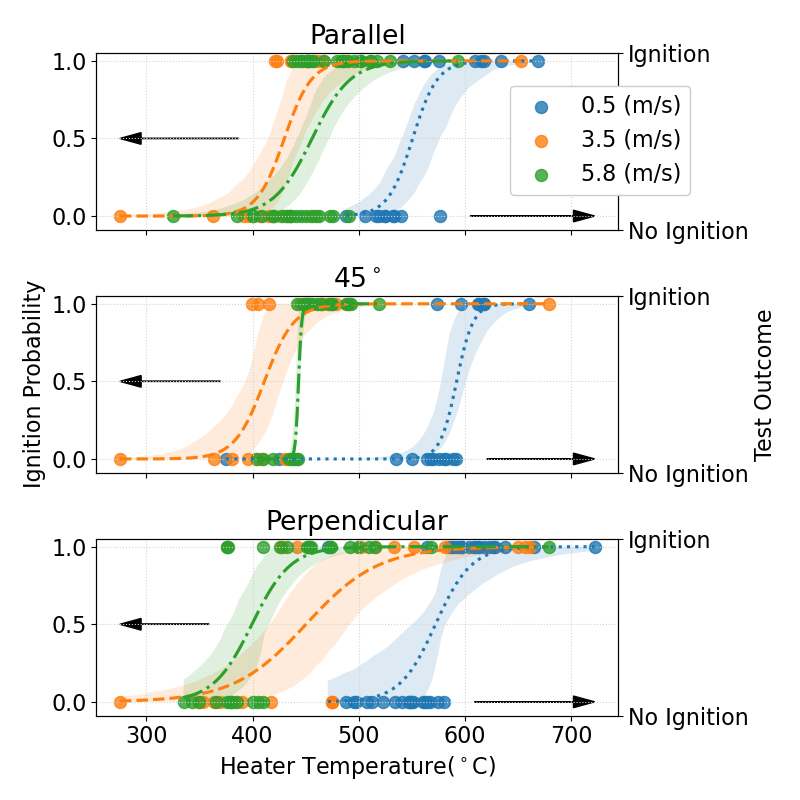
\includegraphics[width=0.5\columnwidth]{Figures/heat_angle_hist_names.png}
            \caption{Ignition or no ignition outcomes of tests at different bulk wind speeds with respect to heater orientation. Markers indicate the outcome of each test and the curves show the logistic regression of each test group. The shaded regions show 95\% confidence intervals for each regression.}
            \label{fig:heaterAngle}
        \end{figure}
    The three different sets of data in each plot are the results for the experiments with three wind speeds. Table~\ref{tab:fiftyTemp} shows the heater temperatures estimated to produce a 50\% ignition probability for the results shown in Figure~\ref{fig:heaterAngle}.
        \rowcolors{2}{gray!25}{white}
            \begin{table}[hpbt]
                \normalsize
                \caption{Heater temperature required to achieve 50\% ignition probability for the wind speeds and heater angles tested.}
                \centering
                \begin{tabular}{crrr}
                    \rowcolor{gray!50}
                   U\textsubscript{bulk} (\si{\meter\per\second}) & 0 \si{\degree} (\si{\celsius}) & 45\si{\degree} (\si{\celsius}) & 90\si{\degree} (\si{\celsius})\\
                    \hline
                    0.5  & 551 & 592 & 571\\
                    3.5  & 430 & 411 & 450\\
                    5.8  & 456 & 443 & 399
                \end{tabular}
                \label{tab:fiftyTemp}
            \end{table}
    Three observations are noted for the results in Figure~\ref{fig:heaterAngle} and Table~\ref{tab:fiftyTemp}. 
    First, the ignition probability for the 0.5\si{\meter\per\second} cases are similar to previously published results for a similar fuel bed and apparatus with measured wind speeds of 0.1\si{\meter\per\second}\cite{Bean2021}. Second, increasing the wind speed beyond 0.5\si{\meter\per\second} increased the ignition probability. This observation is consistent with previously reported work~\cite{Ganteaume2009, Matvienko2018} that showed that the presence of wind can increase the likelihood of ignition. What has not been quantified previously is the magnitude of the difference in ignition probability due to wind speed. For example, in tests with the heater oriented parallel to the flow, a heater temperature expected to produce ignition 25\% of the time at a wind speed of 0.5\si{\meter\per\second} is anticipated to produce ignitions for greater than 99\% of tests at 3.5\si{\meter\per\second} and 5.8\si{\meter\per\second}. The difference is even more pronounced for the 45\si{\degree} and perpendicular orientations where heater temperatures expected to result in ignition less than 1\% of tests at 0.5\si{\meter\per\second} have an ignition probability of over 99\% at 5.8\si{\meter\per\second}. This observation illustrates that an increase in wind speed that is relatively modest (compared to winds often accompanying wildfires) can shift fuel bed ignition risk from minimal to very likely with no other changes in conditions.
    
    The third observation from Figure~\ref{fig:heaterAngle} and Table~\ref{tab:fiftyTemp} is that while an increase in wind speed from 0.5\si{\meter\per\second} to 3.5\si{\meter\per\second} resulted in an increase in ignition probability for all heater angles, an increase from 3.5\si{\meter\per\second} to 5.8\si{\meter\per\second} does not. For tests where the heater was perpendicular to the flow (90\si{\degree}) an increase in wind speed led to a decrease in heater temperatures required for ignition. For tests with the heater at 45\si{\degree} to the oncoming flow, ignitions were observed at the lowest temperatures in the 3.5\si{\meter\per\second} case. For the parallel heater case the difference in ignition between the 3.5\si{\meter\per\second}, and 5.8\si{\meter\per\second} cases were not statistically significant. These trends in ignition propensity suggest that there is a threshold for ignition enhancement that depends on both wind speed and orientation of the wind with respect to the firebrand. A threshold for an optimum wind speed for inducing ignition has been postulated~\cite{Plucinski2008} but this is one of the first studies to confirm its existence and dependence on the orientation of the wind.
    
    Figure~\ref{fig:windSpeed} shows the data reported in Figure~\ref{fig:heaterAngle} but organized to more easily highlight sensitivities of ignition behavior for the different heater angles for a constant wind speed. Three observations are noted. First, differences in ignition probability were not statistically significant for the various heater orientations and a wind speed of 0.5\si{\meter\per\second}. This suggests, as anticipated, that for near quiescent conditions the orientation of the firebrand is less important than the temperature of the firebrand. Second, for the 3.5\si{\meter\per\second} tests there was not a statistically significant difference in ignition temperatures for the parallel and 45\si{\degree} heater orientations, but there is a statistically significant difference at the 5.8 \si{\meter\per\second} case. The differences in sensitivities between the two wind speeds is attributed to the lowest temperature required for ignition (maximum ignition enhancement) occurring for a wind speed of 3.5\si{\meter\per\second} for the 45\si{\degree} orientation. The maximum enhancement of ignition for the perpendicular case appears to occur at a wind speed above 3.5\si{\meter\per\second}. The third observation is that changing the angle of the heater relative to the wind direction has less of an influence on ignition behavior than changing the wind speed.
    Thus, for a fixed heater temperature, an increase in wind speed will yield a larger increase in ignition probability when compared to changing the firebrand orientation. This is only true, however, up to the wind speed that produces the greatest likelihood of ignition. 
    
    At and above the wind speed that produces the greatest likelihood of ignition for a given firebrand orientation, an increase in ignition will only occur if the angle between the firebrand and wind is increased to become more perpendicular to the flow. 
    The aforementioned observations affirm that both the wind speed and direction can alter the likelihood of flaming ignition of a fuel bed. What is unclear, thus far, are the specific physical processes that promote or retard ignition as the wind speed is increased or the heater angle is changed.  
    
        \begin{figure}[hpbt]
            \centering
            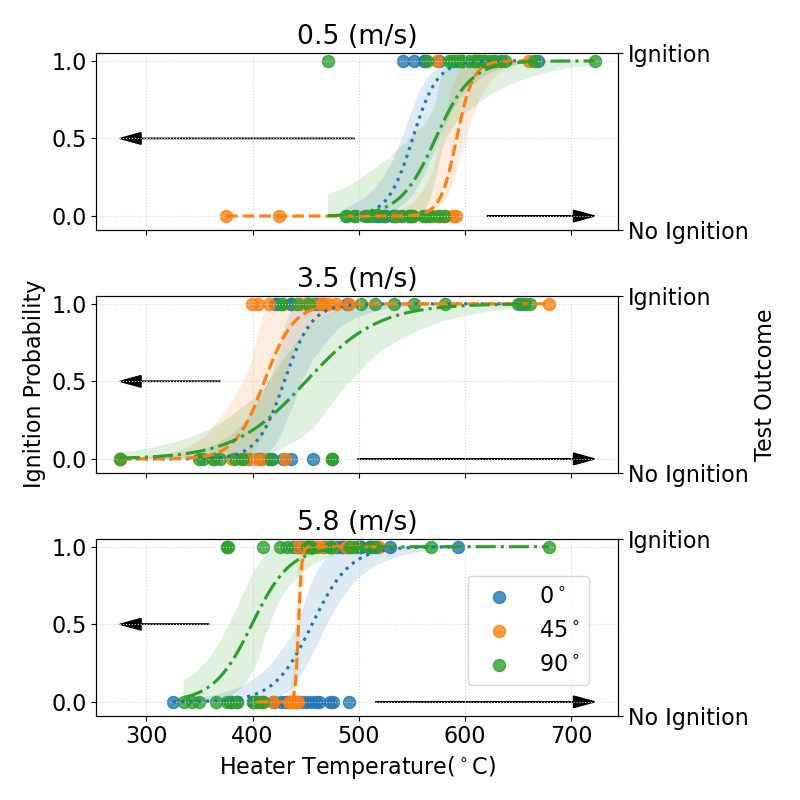
\includegraphics[width=0.5\columnwidth]{Figures/stacked_wind_speed.png}
            \caption{Ignition or no ignition outcomes of tests at different heater angles with respect to wind speed. Markers indicate the outcome of each test and the curves show the logistic regression of each test group. The shaded regions show 95\% confidence intervals for each regression.}
            \label{fig:windSpeed}
        \end{figure}
    
    In contrast to the observed sensitivities of wind speed on ignition probability the time to ignition is more sensitive to the heater orientation than the wind speed. Figure~\ref{fig:histogramFigure} shows histograms of the time to ignition (i.e., occurrence of flames) for each test where ignition was observed. The wind speed increases from the top plot to the bottom plot and the color of each group in the plot represents the different heater angles. Note that the time to ignition axis is log-scale. Three observations are noted about the time to flaming ignition. First, the times to ignition for the 3.5\si{\meter\per\second}, and 5.8\si{\meter\per\second} wind speeds often are sufficiently long (i.e., \textgreater 100\si{\second}) enough to suggest that the fuel beds may be igniting in a smoldering mode and then transition to flaming. Second, for the 0.5\si{\meter\per\second} tests the difference in time to ignition between the heater angles are much smaller than for the other two wind speeds. Third, for the 3.5\si{\meter\per\second}, and 5.8\si{\meter\per\second} cases ignition times are typically longest when the heater is oriented parallel to the flow. The shortest times to ignition typically occurred when the heater was perpendicular to the flow. The sensitivity of time to ignition to different heater angles suggests that the ignition process changes as the heater angle changes.
        \begin{figure}[hpbt]
            \centering
            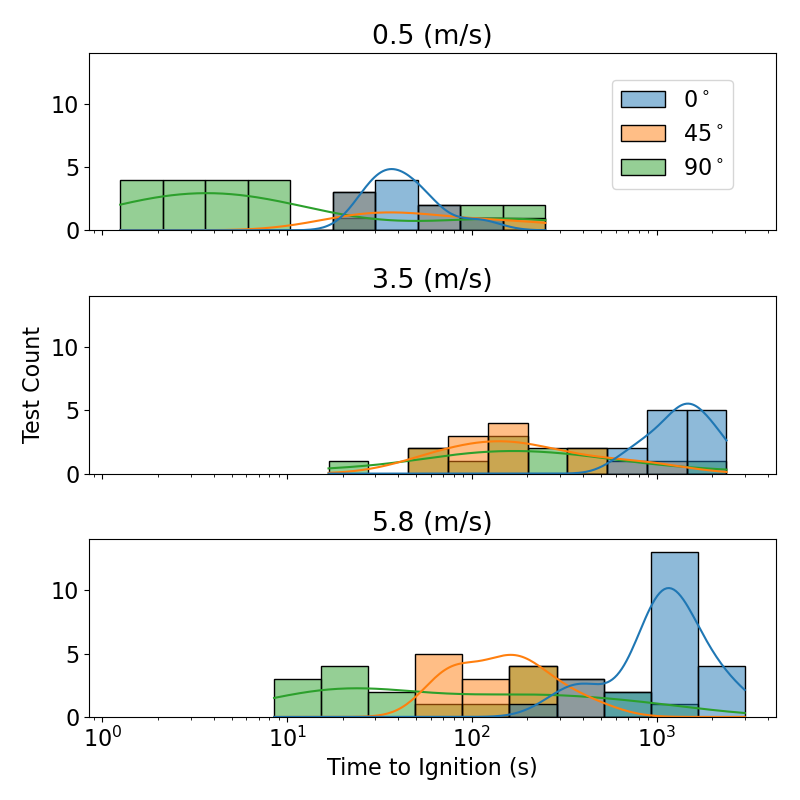
\includegraphics[width=0.5\columnwidth]{Figures/stacked_speed_hist.png}
            \caption{Histogram of time to flaming ignition for each test group. Wind speed increased from top to bottom with color indicating different heater angles.}
            \label{fig:histogramFigure}
        \end{figure}
    
    High speed images were recorded for a subset of test configurations to provide more insight into changes in ignition location resulting from changes in heater angle. Figure~\ref{fig:ignitionImages} shows images of the initial flame visible during tests of three different heater angles. A heater temperature of 450\si{\celsius} and a wind speed of 5.8\si{\meter\per\second} were used for all tests. Consistency in the location of ignition was verified by comparing images from three different ignition events for each of the heater angles. For tests where the heater was oriented at either 45\si{\degree} or perpendicular to the flow (Figure~\ref{subfig:perpendicularHeater},~\ref{subfig:45Heater}) ignition was observed to occur on the upwind side of the heater near the fuel bed. For the parallel heater orientation (Figure~\ref{subfig:parallelHeater}) ignition was observed underneath the heater in a cavity. The cavity was formed by the pyrolysis of the fuel bed. Specifically, ignition occurred at the downstream side of the cavity in the fuel bed. 
        \begin{figure}[hpbt]
             \centering
             \begin{subfigure}[b]{0.5\columnwidth}
                 \centering
                 \begin{tikzpicture}
                 \node(a){
                 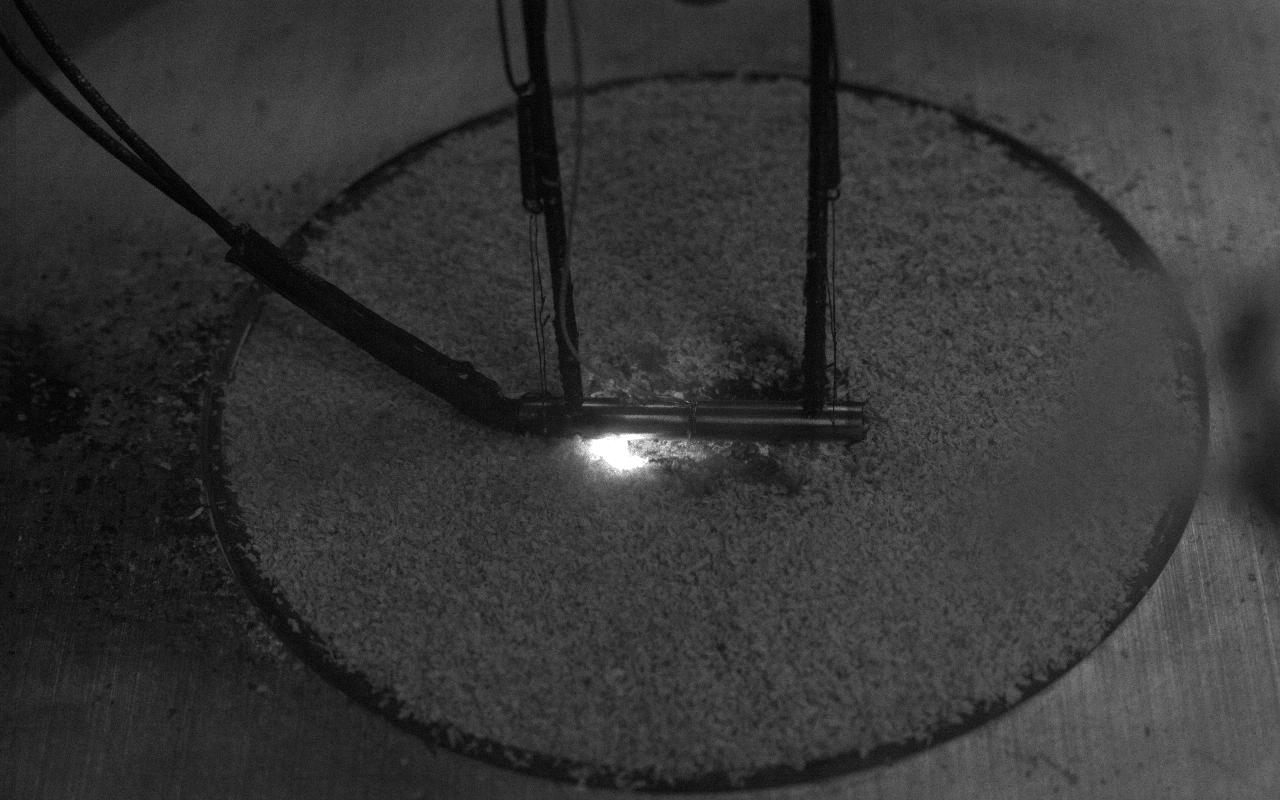
\includegraphics[width=0.75\columnwidth, trim={12cm 5cm 10cm 5cm}, clip]{Figures/5ms_0_heater_450.png}};
                 \node at(a.center)[draw, red, dashed, line width=1pt, rectangle, minimum width=65pt, minimum height=14pt,rotate=-1, yshift=-18pt, xshift=2pt]{};
                 \draw[->, thick, white] (1.5, 1.25) -- node [midway,above] {Wind Direction}(-1.2, 1.25);
                 \end{tikzpicture}
                 \caption{Parallel}
                 \label{subfig:parallelHeater}
             \end{subfigure}
             \hfill
             \begin{subfigure}[b]{0.5\columnwidth}
                 \centering
                 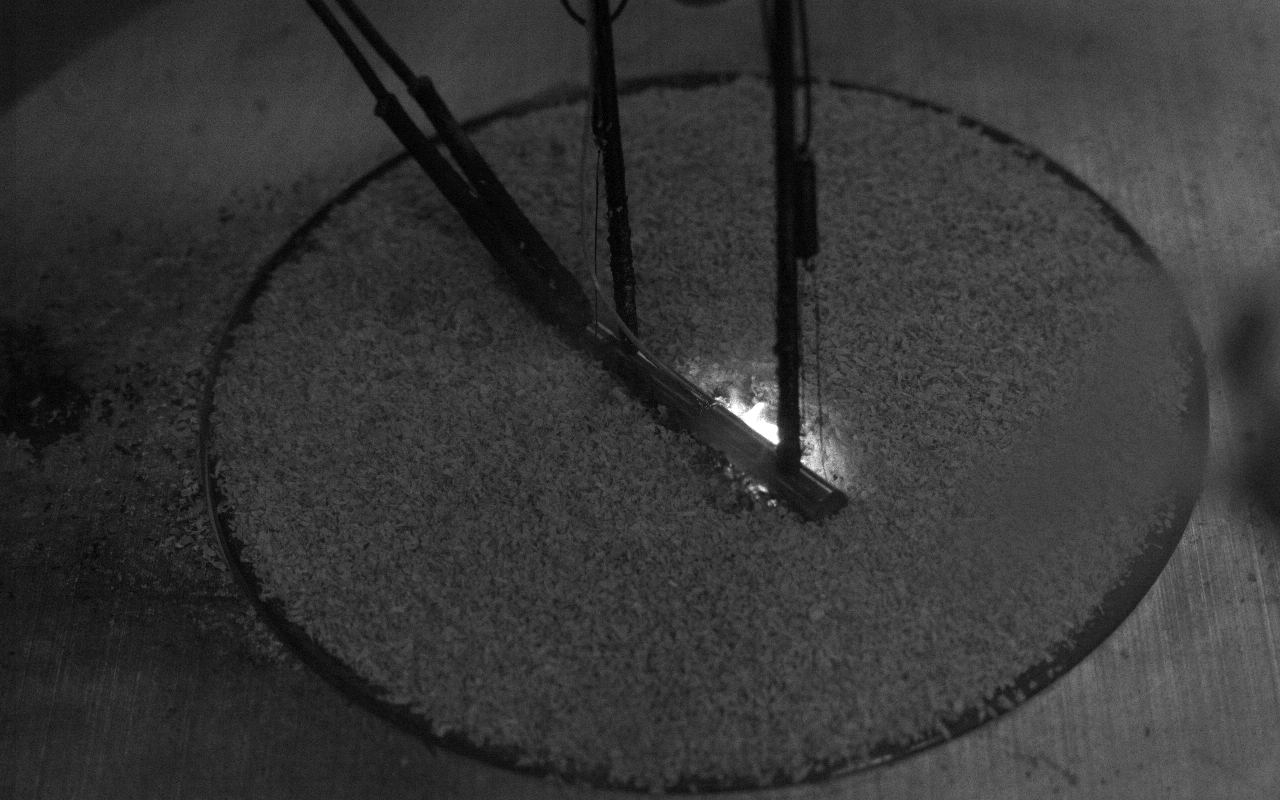
\includegraphics[width=0.75\columnwidth, trim={12cm 5cm 10cm 5cm}, clip]{Figures/5ms_45_heater_450.png}
                 \caption{45\si{\degree}}
                 \label{subfig:45Heater}
             \end{subfigure}
             \hfill
             \begin{subfigure}[b]{0.5\columnwidth}
                 \centering
                 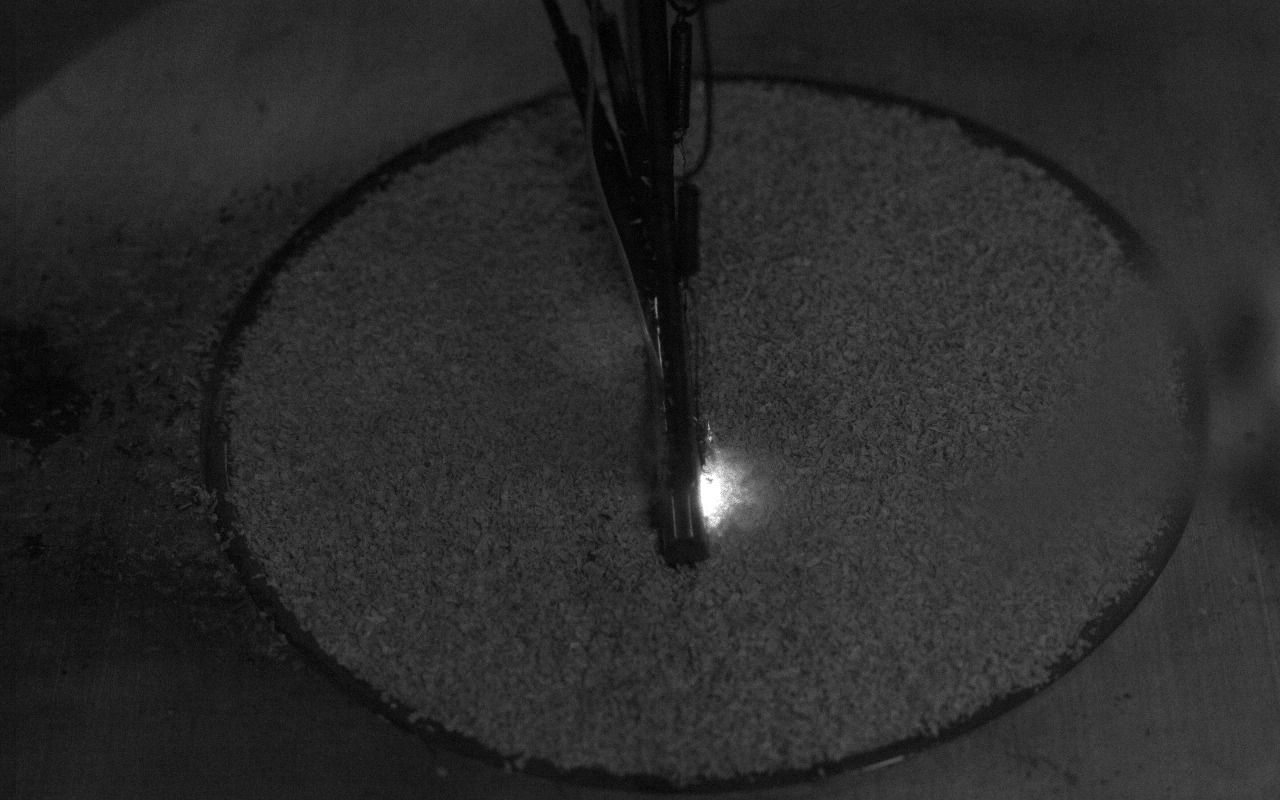
\includegraphics[width=0.75\columnwidth, trim={12cm 5cm 10cm 5cm}, clip]{Figures/5ms_90_heater_450.png}
                 \caption{Perpendicular}
                 \label{subfig:perpendicularHeater}
             \end{subfigure}
                \caption{Representative images of the location of flaming ignition for three different heater angles with a heater temperature of 450\si{\celsius} and a wind speed of 5.8\si{\meter\per\second} from right to left. The dotted rectangle in \ref{subfig:parallelHeater} highlights the cavity formed under the heater during tests.}
                \label{fig:ignitionImages}
        \end{figure}
    Differences in ignition location, and subsequent changes in ignition times, are attributed to changes in the velocity field around the heater as the orientation relative to the wind changes. As the heater is rotated from parallel to perpendicular to the flow, pyrolyzates are more likely to remain near the hottest part of the heater (approximately the center) due to the recirculation zones that form on the upwind side of the heater. When the heater is parallel to the flow pyrolyzates tend to advect away from the heater. Thus, for the perpendicular heater the recirculation zone is anticipated to have the longest pyrolyzate residence time. The pyrolyzates are also anticipated to remain near the highest temperature region of the heater. This explantion is consistent with the observation that tests where the heater is oriented perpendicular to the flow typically ignited at lower temperatures than the other orientations, as shown in Figure~\ref{fig:windSpeed}.
    
    Considering the aforementioned importance of pyrolyzate residence time on ignition enhancement, it is not immediately clear how the threshold for ignition is lowered with an increase of wind for tests where the heater is parallel to the wind direction. When the heater is positioned parallel to the flow with wind, the pyrolyzates tend to advect away from the hot regions of the heater. However, as previously noted, ignitions for the parallel case occur inside a cavity that forms underneath the heater. The fluid flow that develops with this cavity is anticipated to lead to longer residence times for pyrolyzates. The absence of a sufficient residence times until a cavity of sufficient size forms appears to be the major reason for differences in the time to ignition for the various heater orientations.
    

    Further insights into recirculation zones that form near the heater and the impact on residence times of pyrolyzates are gained from computational results. Figure~\ref{fig:CFDImages} shows streamlines passing though the pyrolysis release zones and the temperature distribution for regions where pyrolyzates are present (i.e., $\phi>$0.05) for the three heater orientations at a wind speed of 5.8\si{\meter\per\second}. The images shown in Figure~\ref{fig:CFDImages} correspond to 1\si{\second} after the release of pyrolyzates. While typical ignition times are significantly longer than 1\si{\second}, the results still provide insight into the controlling fluid mechanics. The streamlines shown in Figure~\ref{fig:CFDImages} confirm that a recirculation zone is present near the hottest region of the heater when the orientation is perpendicular or 45\si{\degree} with respect to the wind direction. The presence of recirculation zones is further supported by the presence of pyrolyzates upstream of the heater in Figures~\ref{subfig:45CFD},\ref{subfig:perpendicularCFD}.
           \begin{figure}[hpbt]
             \centering
             \begin{subfigure}[b]{\columnwidth}
                 \centering
                 \begin{tikzpicture}
                     \node{
                     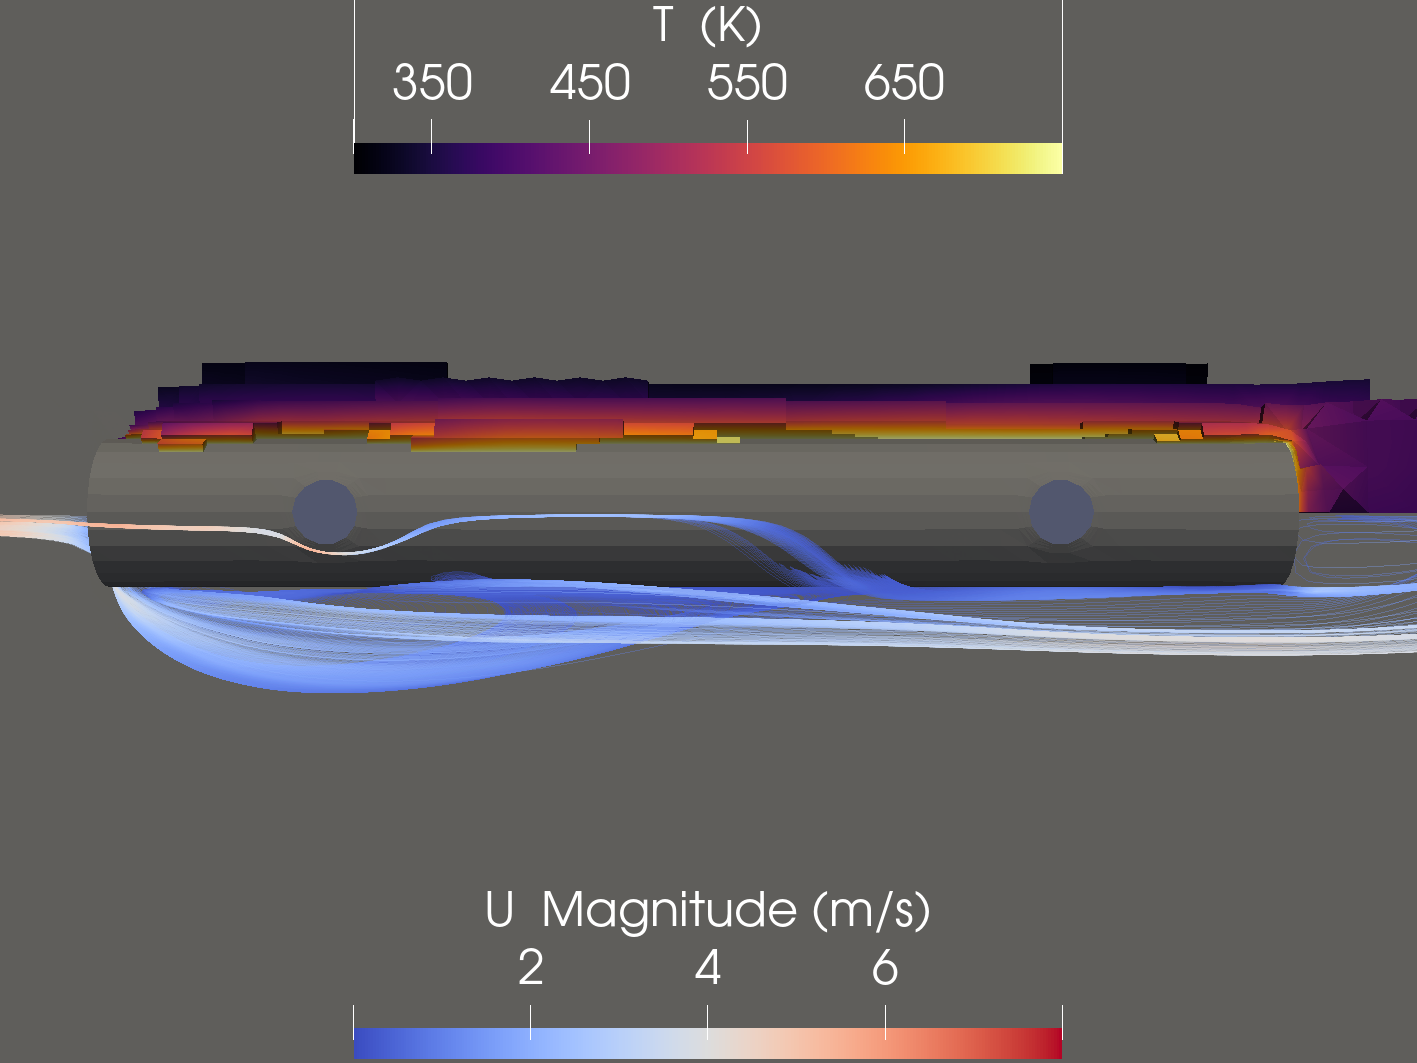
\includegraphics[width=0.45\columnwidth]{Figures/parallel_cfd_plot.png}};
                     \draw[-, dotted, very thick, red] (-2.5, 0.05) -- (2.5, 0.05);
                 \end{tikzpicture}
                 \caption{Parallel}
                 \label{subfig:parallelCFD}
             \end{subfigure}
             \hfill
             \begin{subfigure}[b]{\columnwidth}
                 \centering
                 \begin{tikzpicture}
                     \node{
                     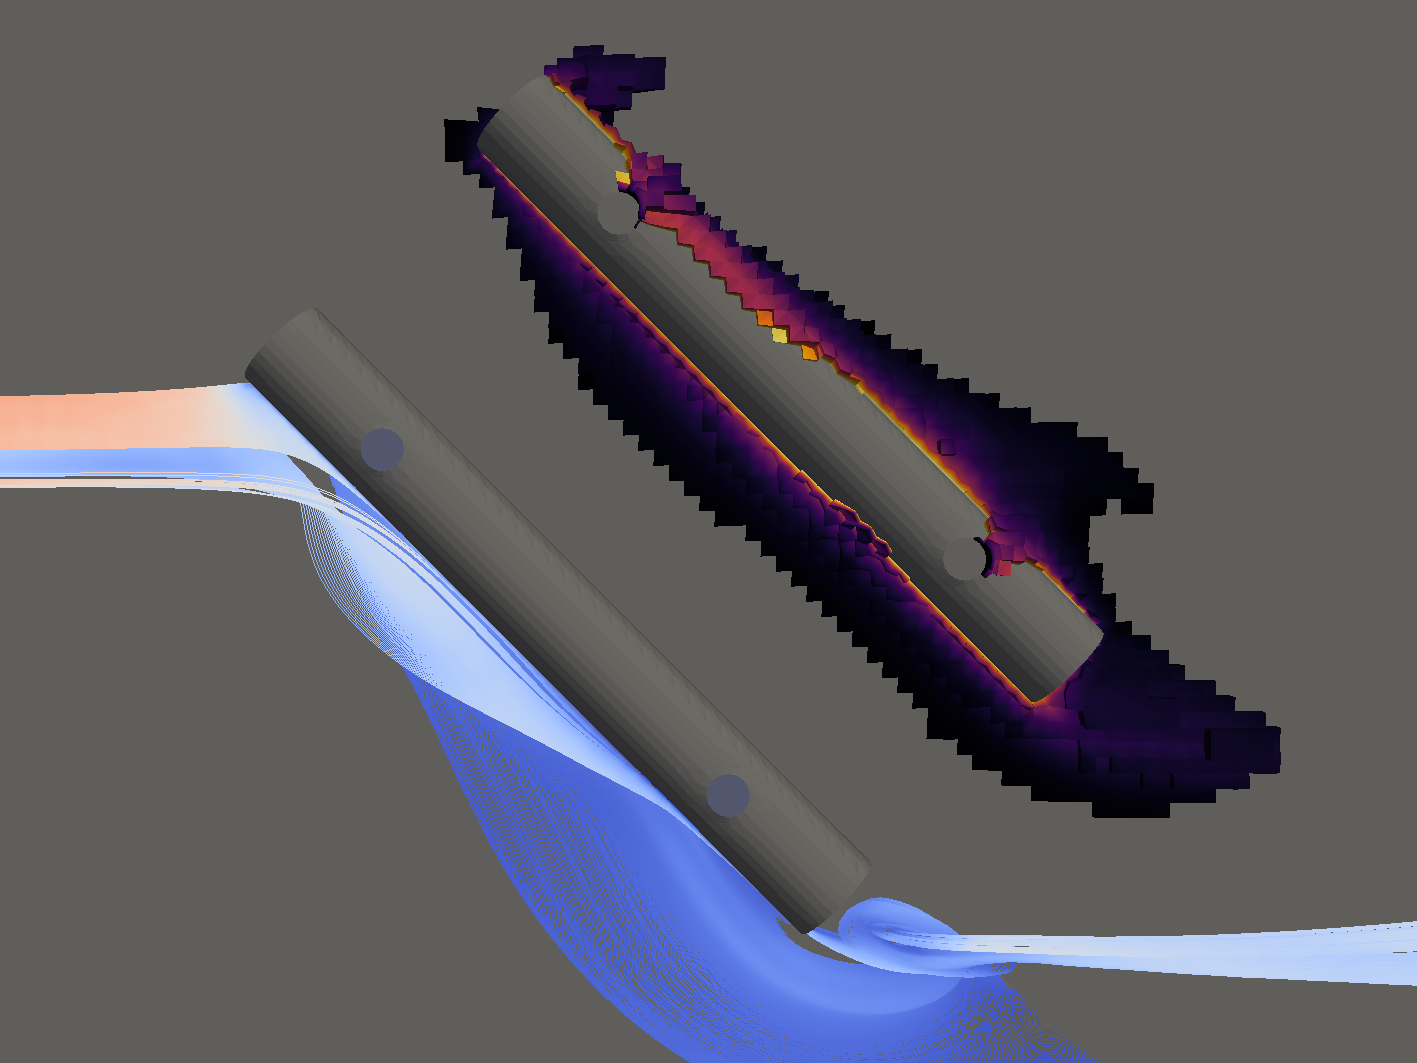
\includegraphics[width=0.45\columnwidth]{Figures/45_cfd_plot.png}};
                     \draw[-, dotted, very thick, red] (-2.1, 1.9) -- (0.9, -1.2) -- (2.5, -1.2);
                 \end{tikzpicture}
                 \caption{45\si{\degree}}
                 \label{subfig:45CFD}
             \end{subfigure}
             \hfill
             \begin{subfigure}[b]{\columnwidth}
                 \centering
                 \begin{tikzpicture}
                     \node{
                     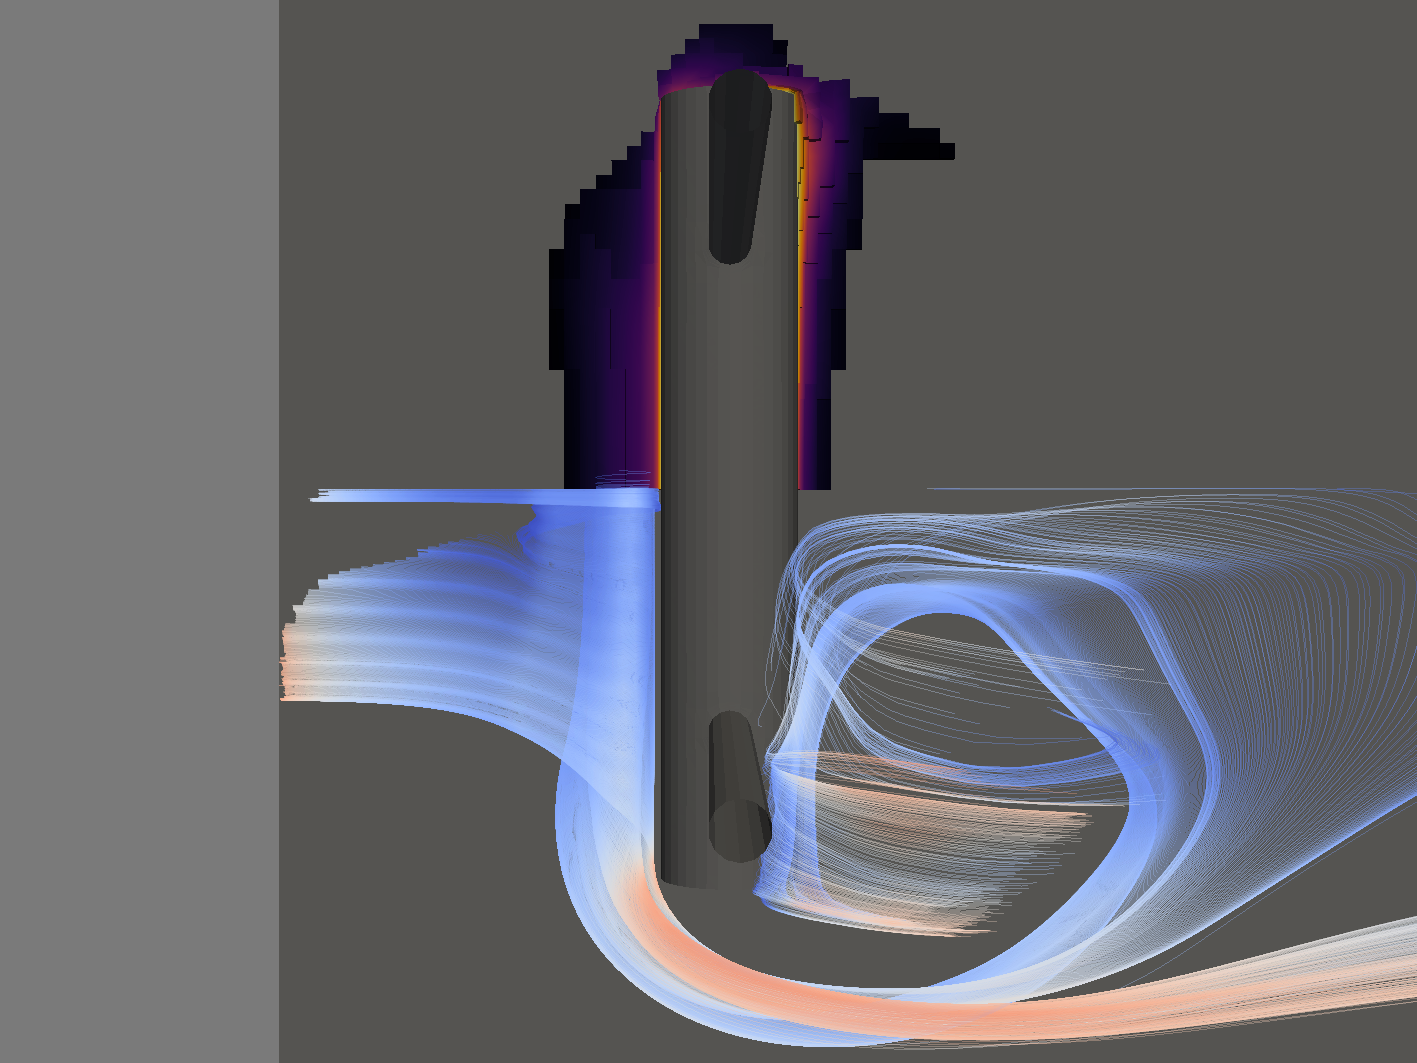
\includegraphics[width=0.45\columnwidth, trim={10cm 0cm 0cm 0cm}, clip]{Figures/90_cfd_plot.png}};
                    \draw[-, dotted, very thick, red] (-2.5, 0.18) -- (2.5, 0.18);
                 \end{tikzpicture}
                 \caption{Perpendicular}
                 \label{subfig:perpendicularCFD}
             \end{subfigure}
                \caption{CFD results showing pyrolyzate distribution and streamlines for a wind speed of 5.8\si{\meter\per\second}. The top half of each image shows the temperature distribution of pyrolyzates in regions where pyrolyzates are present (i.e., $\phi>$0.05). The bottom half of each image shows the streamlines, with the color scale representing velocity magnitude, passing through the pyrolyzate release region. Panel \ref{subfig:45CFD} shows a duplicated heater across the dotted line.}
                \label{fig:CFDImages}
        \end{figure}
    Perhaps unexpected are the characteristics of the region of the fluid anticipated to be capable of ignition ($\Phi>0.85$). For both the parallel and 45\si{\degree} heater orientation the total volume of ignitable pyrolyzates are between 4 and 6 times larger than the perpendicular heater orientation. The average temperature 3\%-5\% larger in the parallel and 45\si{\degree} heater orientations. These results suggest that the gas and temperature conditions favor ignition when the heater is not perpendicular to the flow. However, the residence time of the flammable mixture favors ignition when the heater is perpendicular to the flow. Estimates of residence time are made using the ratio of the average velocity magnitude of the pyrolysis gases with $\Phi>0.85$ and the mass release rate of the pyrolyzates from the fuel bed estimates. The average velocity of the pyrolyzates serves as a proxy for removal of combustible gases from the high temperature zone near the heater. The estimated residence time of the pyrolyzates in the perpendicular heater orientation is more than 25 times longer when compared to the parallel heater orientation and 15 times longer when compared to the 45\si{\degree} heater orientation. The differences in residence times for the three heater orientations align with those for ignition probability supporting the previous assertion that combinations of wind and geometry that facilitate long residence times ignite more readily.
    
    The correlation between time to ignition, ignition temperatures, and ignition locations indicates that ignition events are sensitive to the residence time of pyrolyzates in a high temperature zone. In other words, a firebrand is much more likely to ignite a fuel bed if the wind speed and geometry of the firebrand or firebrands promote extended residence times of pyrolyzates in a low velocity recirculation zone near the firebrand.
   
\section{Summary and Conclusions}
\label{sec:summary2}
    Flaming ignition tests were conducted for surrogate fuel beds made of Douglas-fir particles.
    Ignition was induced by a cartridge heater, which served as a surrogate firebrand. The heater was maintained at a fixed temperature throughout each test, thus allowing sensitivities of ignition to wind speed and orientation to be further understood. The ignition probability, time to ignition, high speed imagery, and CFD results were used to quantify sensitivities to ignition related to fluid mechanics around the firebrand and fuel bed as controlled by the wind speed and heater angle. The specific conclusions of this work are as follows:
        \begin{enumerate}
            \item
            An increase in wind speed above quiescent conditions reduces the temperature required for the flaming ignition of a fuel bed. For example, an increase in wind speed of 3.5\si{\meter\per\second} from quiescent increases the ignition probability of a fuel bed from under 30\% to roughly 100\%. However, a linear increase in wind speed does not result in a linear increase in ignition probability. Thresholds in wind speed exist above which temperatures required to achieve ignition actually increase. For example, when the wind is oriented 45\si{\degree} from the heater centerline increasing the wind from quiescent to 3.5\si{\meter\per\second} reduces the temperature required for ignition probability by 30\%. However, increasing the wind speed from quiescent to 5.8\si{\meter\per\second} reduces the temperature required for ignition by only 25\%. Presumably these thresholds occur because of reductions in residence time. 
            
            \item The temperatures at which ignition occurs for porous fuel beds is sensitive to the orientation of a firebrand relative to the wind direction. Higher temperatures are typically required for ignition for a heater parallel to the flow compared to 45\si{\degree} and perpendicular to the flow. This sensitivity attributed to differences in recirculation zones and residence times of air and pyrolyzates near the hottest region of the heater. Thus, predictions of ignition probabilities that consider wind may need to include both wind speed and orientation to obtain sufficient accuracy.
            
            \item Times to flaming ignition of porous fuel beds are sensitive to the firebrand/heater angle in the presence of wind.
            The parallel heater orientation ignites at the longest time followed by the 45\si{\degree} case with the perpendicular cases igniting in the shortest amount of time. High speed images indicate that ignition typically occurrs in regions where recirculation zones occur, as shown in CFD calculations. The heightened propensity to ignition is attributed to increased residence times of pyrolyzates in the recirculation zones as supported by calculations.
        \end{enumerate}
    The conclusions of this work show that ignition is favored when a firebrand(s) land on a fuel bed under wind speeds and orientations that promote greater residence times of pyrolyzates near a high temperature region of firebrands. It was observed that increases of wind speed, of a magnitude that may commonly occur during wildfires, can increase the probability of fuel bed ignition from very unlikely to a near certainty regardless of the ember orientation to the wind. This highlights the increased risk of spot fires due to ignition of fuel beds that accompanies wind in a wildfire. 
%!TEX root = thesis.tex

\renewcommand{\TheTitle}{Effect of Fuel Bed Composition on Flaming Ignition Probability}
\renewcommand{\TheAuthors}{Derek Bean, David L. Blunck \\ \\ My contributions to this work included the design of the experiments, fabrication of the experimental apparatus, collecting data, data analysis, and preparation of the manuscript.}

\renewcommand{\TheAddress}{
\textbf{Status: In Preparation}\\
Target Journals: Fire Safety Science, Fire Safety Journal, or Fire Technology
}

\PaperHeader{\TheTitle}{\TheAuthors}{\TheAddress}

\chapter{\TheTitle}
\label{part:manuscript3}

\section{Abstract}
\label{sec:abtract3}
    The increasing severity of wildfires and the expansion of the wildland urban interface have placed a greater number of homes at risk for being destroyed by wildfires. Ignition of fuel beds on or near homes by firebrands is a significant source of fire spread and structure loss. Fire prevention and suppression efforts lack an expedient method for estimating the likelihood of ignition for the wide variety of materials around homes. 
        
\section{Introduction}\addvspace{10pt}
\label{sec:introduction3}
    
    The phenomena that occur after an firebrand lands can be further broken down into three categories. First the properties of the firebrand that lands, second the heat transfer between the firebrand, fuel bed, and the surroundings, and third how the fuel bed responds to the heat transfer from the firebrand. The response of the fuel bed to the heat transfer from the the firebrand is influenced by the morphology and chemical composition of the particles in the fuel bed. Fuel bed materials present in wildfires vary significantly in both morphology and chemical composition and knowledge of the effects of each on ignition are qualitative, at best. A previous study evaluated the effects of particle morphology~\cite{Bean2021} and this work seeks to identify how differences in the chemical composition of a fuel bed under attack by firebrands influence the probability of flaming ignition. 
    
    Fuel beds at risk for ignition by firebrands vary significantly in chemical composition which may result in differences in thermal properties and the chemical species produces during pyrolysis. Works considering ignition of fuel beds with varying concentrations of constituents have found significant variation in ignition characteristics. Cellulose fuel beds have been observed to have a lower ignition threshold when compared to grass and pine needles when put in contact by hot metal particles~\cite{Urban2018}. Interestingly, cellulose undergoes pyrolysis at either higher temperatures or later in the heating process than both lignin and hemicellulose~\cite{Yang2007a, Shotorban2018}. This suggests that the lower ignition temperature of cellulose is not due to pyrolysis occurring at lower temperatures, but to the flammability of pyrolyzates produced. 
    
    One method to evaluate the effects of chemical composition on the flammability of pyrolyzates produced, and thus ignition propensity, is through modeling of the pyrolysis process. Efforts to characterize the pyrolysis of biomass have continually improved the understanding of the chemical processes that occur in both the solid and gas phase of pyrolysis products. Recently, more inclusive pyrolysis models have been developed that improve on the initial single step Arrhenius reactions~\cite{DIBLASI199371} and more closely approximate the reactions occurring during combustion of biomass~\cite{Ranzi2008, Debiagi2015, Dhahak2019} based on the initial chemical composition of the fuels. With the development of models that are applicable to a wide range of chemical compositions and environmental factors the possibility of modelling pyrolysis and ignition of fuel beds is possible. Coupling these models with databases, such as the Bioenergy Feedstock Library~\cite{feedstock} (which contains the chemical composition information for a wide variety of materials that may be vulnerable to firebrand attack during a wildfire), predictions of ignition potential may be possible without data from ignition experiments. While currently available tools, like combustion models and composition databases, may be useful individually for understanding fuel bed ignition and pyrolysis, a framework linking the individual resources and knowledge to provide a general model of fuel bed ignition is lacking. Unfortunately, the current level of knowledge on the ignition threshold of materials of variable composition does not facilitate such a framework.
    
    Studies considering ignition have primarily focused on the influence of heat transfer and fuel bed conditions when identifying ignition parameters and the observed sensitivities to fuel bed properties are attributed to both heat transfer and chemistry related processes. The probability of ignition generally increases as the energy content of an firebrand increases~\cite{Hadden2011}. However, further research has indicated that energy content alone is not a sufficient indicator of ignition as a minimum firebrand temperature (a driver of heat flux rates) is also necessary~\cite{Zak2014}. Additionally, heat loss from firebrands to the surroundings has a significant effect on ignition~\cite{Fernandez-Pello2015}. While the aforementioned efforts have focused primarily on the impact of firebrand properties on ignition, efforts focused on the properties of the fuel bed have shown sensitivities to fuel bed material type and particle size~\cite{Urban2018}. Additionally, for fuel beds of constant particle size, an increase in the packing density of the fuel bed resulted in a decrease in the critical heat flux needed for ignition~\cite{Mindykowski2011, Hernandez2017, Rivera2020}. The observed sensitivities to fuel bed properties are likely caused by both heat transfer and chemistry related processes. Changes in the particle size of a fixed material may impact the contact area (e.g., a ball resting on fine sawdust compared to a pile of pine needles) between the firebrand and fuel bed; potentially reducing the amount of heat transferred through conduction as the contact area decreases. Additionally, when considering a fixed particle size fuel bed, changes in chemical composition may change the heat transfer and heating rate of the materials due to changes in the thermal conductivity of the material affecting the ignition properties of the material. For these reasons, knowledge of the effects of chemical composition on ignition, as it relates to thermal and chemical processes, must be addressed to accurately represent ignition properties for the wide range of materials found in fires resulting in home loss.
  
    The objective of this work is to identify how changes in chemical composition of fuel bed materials effect the probability of flaming ignition. It is anticipated that knowledge gained from this study may be used improve the understanding of fuel bed ignition for different fuels and help build a framework for estimating ignition probabilities of different fuels without the need for extensive laboratory testing.



\section{Methods}
\label{sec:methods3}
    The 50\% probability of flaming ignition with respect to the surface temperature of a resistance heater was determined for five different materials in quiescent conditions and at a wind speed of 5.8\si{\meter\per\second}. The fuel bed materials used were Douglas-fir wood, Douglas-fir bark, pine wood, pine bark, wheat straw, and oak wood. These materials were chosen to represent a range of chemical compositions, and are materials that may be subject to firebrand attack in a wildland urban interface fire. Table \ref{tab:composition} shows the estimated chemical composition of the materials based on the Bioenergy Feedstock Library~\cite{feedstock}. To create fuel beds of consistent particle size,  materials were granulated and then sorted such that the particles fit through a screen with openings of 2.1\si{\milli\meter} but not through openings of 0.85\si{\milli\meter}. Once sorted, the materials were oven dried at 103\si{\celsius}.
    \begin{table*}[hpbt]
        \caption{Proportion of cellulose, hemicellulose, and lignin of the materials tested estimated from the Bioenergy Feedstock Library~\cite{feedstock}}
        \centering
        \begin{tabular}{crrrr}
            % \rowcolor{gray!50}
            Material & Cellulose (\%) & Hemicellulose (\%) & Lignin (\%) & Other (\%) \\
            \hline
            Oak Wood         & 45 & 22 & 24 & 9\\
            Douglas-fir Wood & 44 & 22 & 28 & 6\\
            Wheat Straw      & 44 & 27 & 19 & 10\\
            Pine Wood        & 40 & 30 & 20 & 10\\
            Pine Bark        & 39 & 17 & 37 & 7\\
            Douglas-Fir Bark & 26 & 11 & 59 & 4 
        \end{tabular}
        \label{tab:composition}
    \end{table*}
        \begin{table*}[hpbt]
        \caption{Average bulk density of materials for each material and wind speed.}
        \centering
        \begin{tabular}{crr}
            % \rowcolor{gray!50}
            Material & U\textsubscript{bulk} = 0.1\si{\meter\per\second} (\si{\kilogram\per\cubic\meter})& U\textsubscript{bulk} = 5.8\si{\meter\per\second} (\si{\kilogram\per\cubic\meter})\\
            \hline
            Oak Wood         & 344 & 428 \\
            Douglas-fir Wood & 99  & 74 \\
            Wheat Straw      & 85  & 85 \\
            Pine Wood        & 114 & 115 \\
            Pine Bark        & 215 & 172 \\
            Douglas-Fir Bark & 131 & 146  
        \end{tabular}
        \label{tab:composition}
    \end{table*}
    Two experimental apparatus were used to conduct ignition experiments. The experimental apparatus used for the tests in quiescent conditions is shown in Figure~\ref{fig:speciesApparatus}. The quiescent apparatus used a lever arm to hold the cartridge heater in a fixed position the duration of the test. The heater was inserted into the fuel bed approximately half of the heater diameter (3\si{\milli\meter}). Tests conducted with a wind speed of \si{\meter\per\second} were performed using the apparatus shown in Figure~\ref{fig:speciesWindTunnel}. This apparatus was operated inside of a wind tunnel where the heater was lowered using an automated lowering device that maintained a constant pressure equivalent to that of a 10\si{\gram} firebrand landing on the fuel bed. The pressure was monitored and adjusted using a PID control system with force measured by a load cell. For all tests the cartridge heater (firebrand surrogate) used was a 50\si{\milli\meter} long 6.35\si{\milli\meter} diameter cartridge heater.
        \begin{figure}[htpb]
        \centering
        \resizebox{\figureWidthSet}{!}{%
        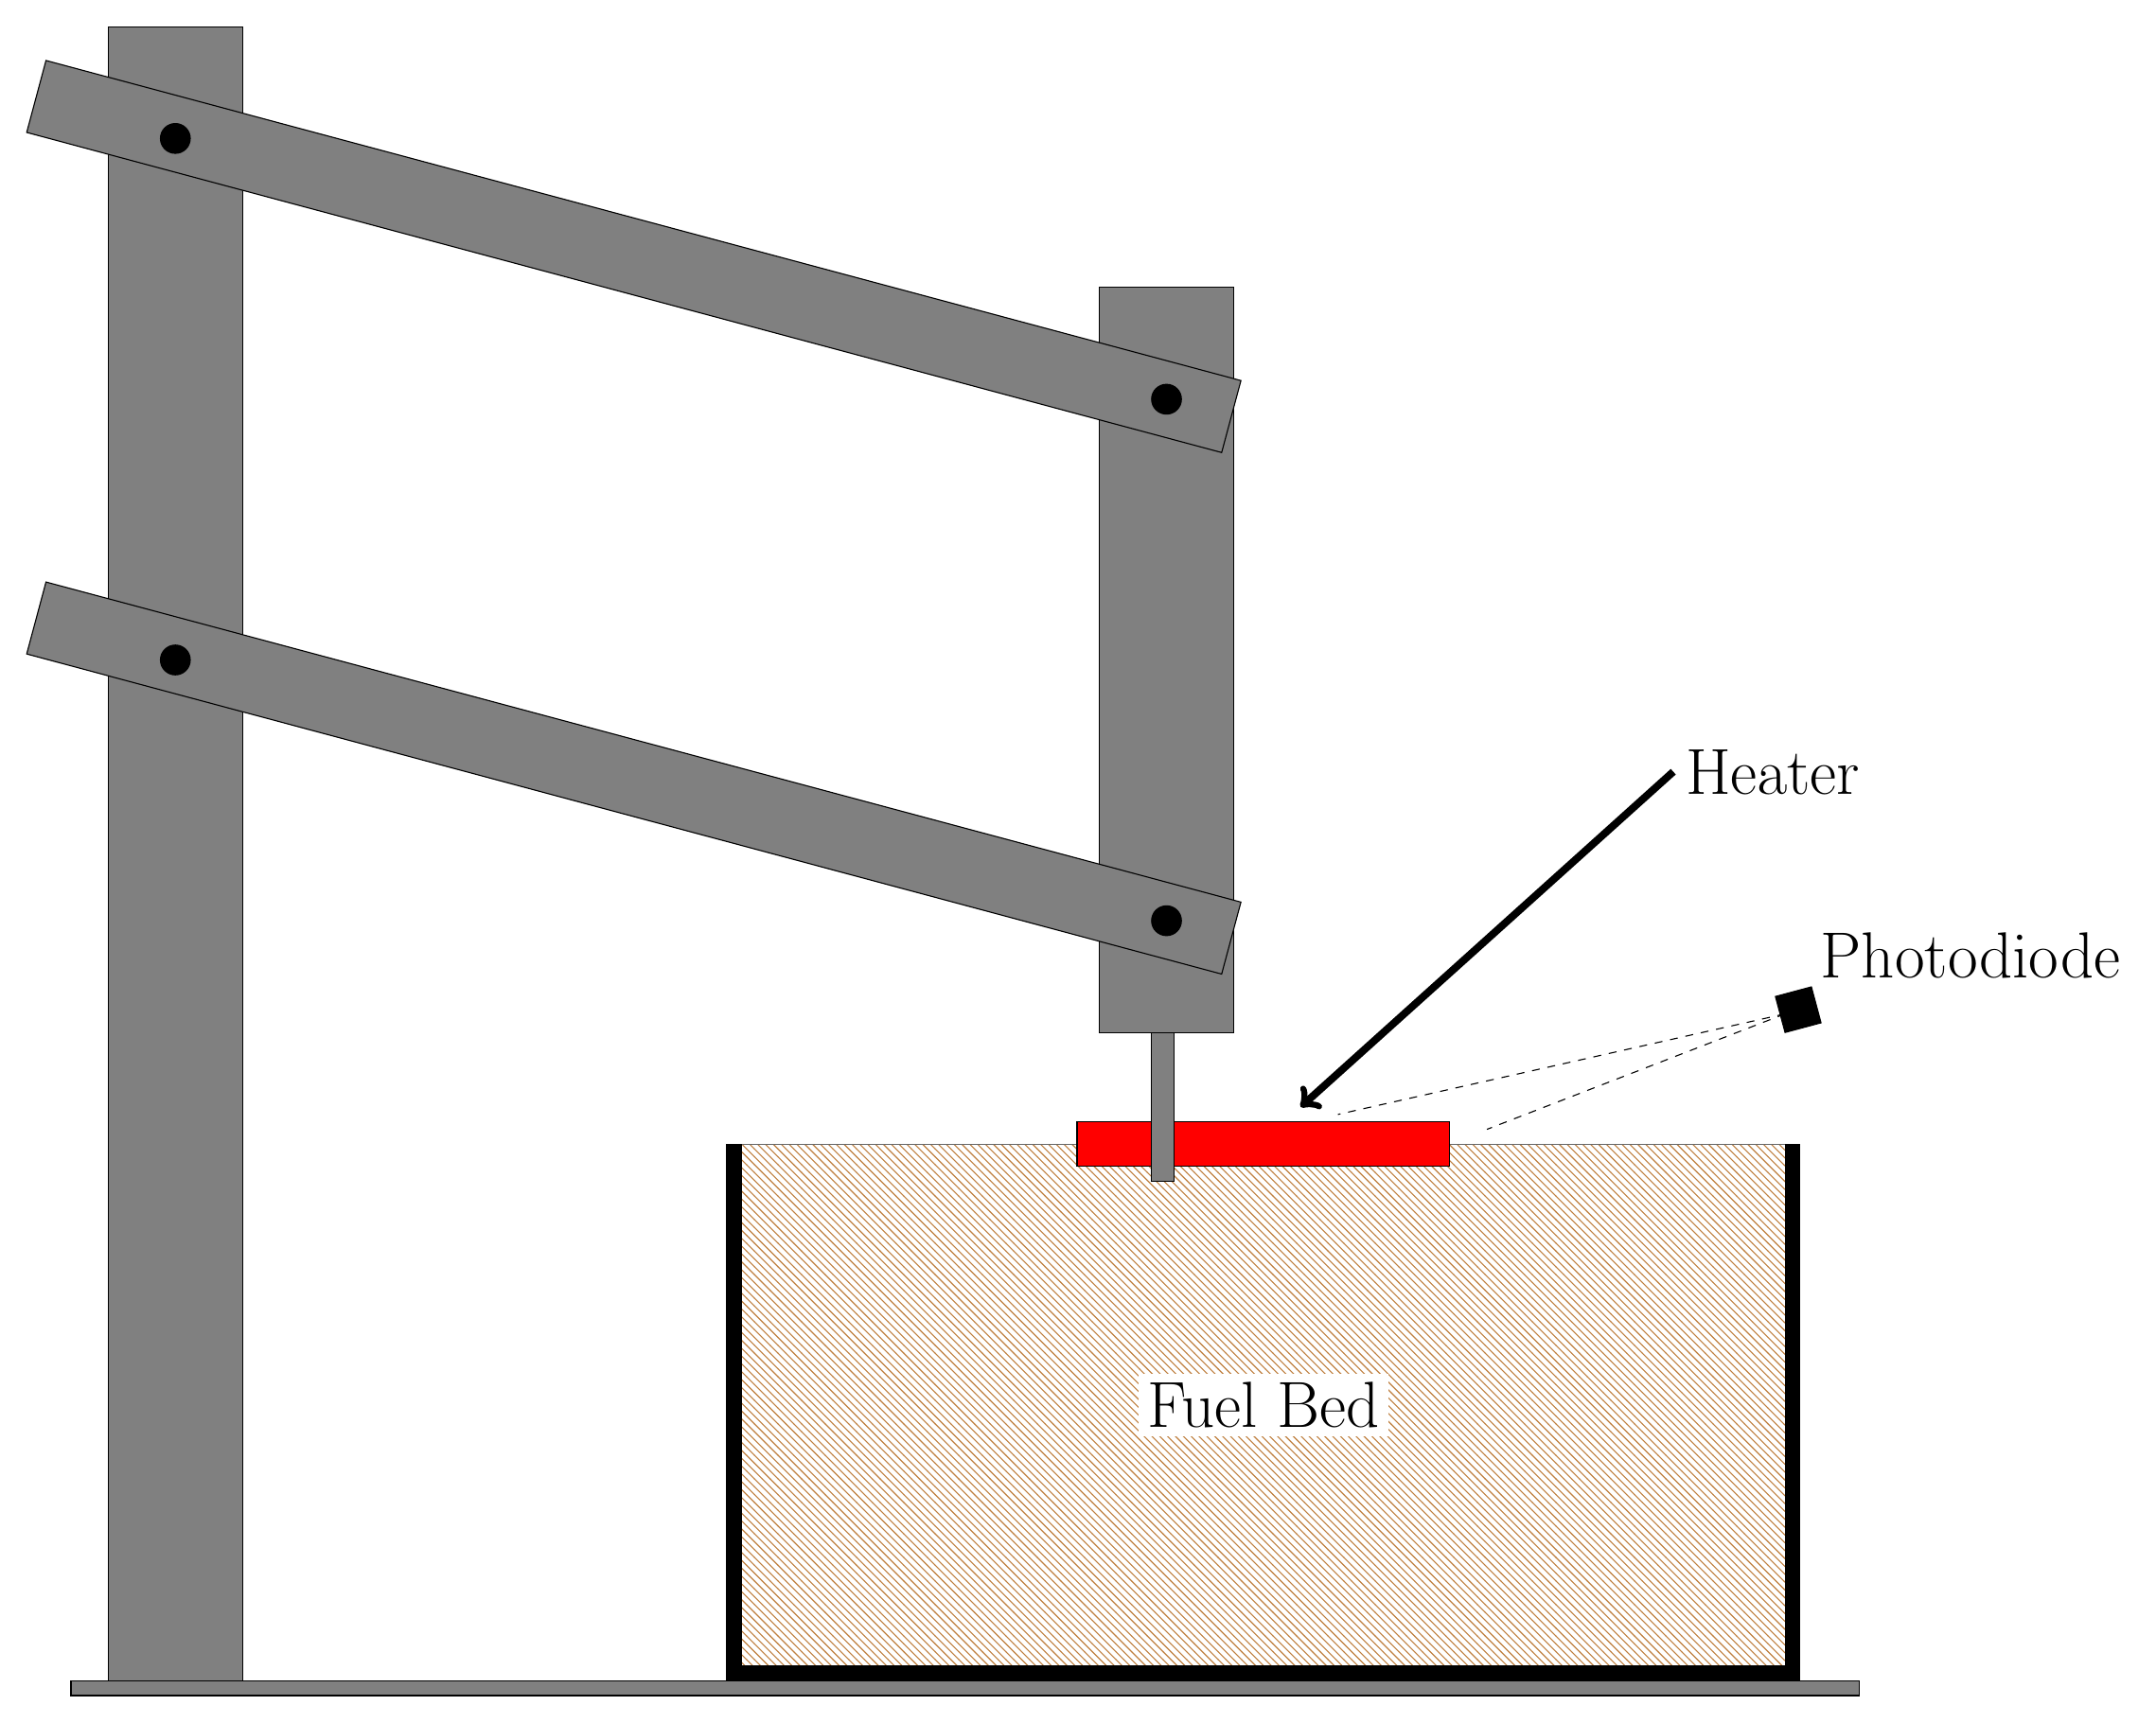
\begin{tikzpicture}
            \filldraw [draw=black!60, pattern=north west lines, pattern color= brown] (0, 0) rectangle (140mm, 70mm) node[pos=0.5, fill=white] {\Huge Fuel Bed}; 
            \filldraw[] (0mm, -2mm) rectangle (140mm,0mm) node[rotate=-90, pos=0.5] {};
            \filldraw[] (-2mm, -2mm) rectangle (0mm,70mm) node[rotate=-90, pos=0.5] {};
            \filldraw[] (140mm, 70mm) rectangle (142mm,-2mm) node[rotate=-90, pos=0.5] {};
            \filldraw [fill=red, draw=black] (45mm, 67mm) rectangle (95mm, 73mm) {}; 
            \filldraw [draw=black, fill=black!50] (55mm, 65mm) rectangle (58mm, 85mm) {};
            \filldraw [draw=black, fill=black!50] (66mm, 85mm) rectangle (48mm, 185mm) {};
            \filldraw [draw=black, fill=black!50] (-85mm, 220mm) rectangle (-67mm, -2mm) {};
            \filldraw [draw=black, fill=black!50, rotate around={-15:(57mm, 100mm)}] (66mm, 95mm) rectangle (-100mm, 105mm) {};
            \filldraw [draw=black, fill=black!50, rotate around={-15:(57mm, 170mm)}] (66mm, 165mm) rectangle (-100mm, 175mm) {};
            \filldraw [draw=black, fill=black!50] (-90mm, -2mm) rectangle (150mm, -4mm) {};
            \filldraw (57mm, 170mm) circle (2mm);
            \filldraw (57mm, 100mm) circle (2mm);
            \filldraw (-76mm, 205mm) circle (2mm);
            \filldraw (-76mm, 135mm) circle (2mm);
            \filldraw [rotate around={15:(140mm, 85mm)}] (140mm, 85mm) rectangle (145mm, 90mm) node[above right] {\Huge Photodiode};
            \draw [<-, line width=1mm] (75mm, 75mm) -- (125mm, 120mm) node[right] {\Huge Heater};
            \draw [dashed] (140mm, 87.5mm) -- (100mm, 72mm);
            \draw [dashed] (140mm, 87.5mm) -- (80mm, 74mm);
        \end{tikzpicture}
        }
        \caption{Experimental apparatus for the ignition tests. The lever arm used to lower the apparatus into the fuel bed, the fuel bed size relative to the heater, and the location of the photodiode are illustrated.}
        \label{fig:speciesApparatus}
    \end{figure}
    The temperature of the heater was recorded with a type-K thermocouple for the duration of each test. The temperature of the heater for ranged from 250\si{\celsius} to 750\si{\celsius} and was controlled using PID control logic implemented in LabVIEW. The PID controller kept the heater temperature within 6\% of the setpoint for the duration of the tests. The temperature setpoints of the resistance heater were determined using the three-phase optimal design procedure to efficiently determine the desired ignition probability for the number of tests conducted~\cite{Wu2014}. For tests where flaming ignition did not occur data was recorded for 3000\si{\second} or until the reaction front of the smoldering material reached the edge of the test container. The fixed position of the cartridge heater and the use of the cartridge heater was implemented to maintain consistency between tests of the same material and between test series of different materials. The use of the cartridge heater and the fixed position is not necessarily representative of a burning firebrand landing on the fuel bed but the consistency of surface temperatures, ability to record temperature, and consistent contact with the fuel bed are essential for comparing results across test series and materials. For the quiescent tests flaming ignition was detected with the use of a BPX 65 photodiode sampled at 1 kHz. If the intensity detected rose above a set threshold flaming ignition was said to occur. For the wind tunnel tests flaming ignition was determined from the rising temperature of the cartridge heater in the presence of flame. Visual detection of flames was also used in cohort with the photodiode measurements. The 50\% probability of ignition was determined from a logistic regression on the outcomes of 25 ignition tests conducted for each of the materials for which flaming ignition was observed. The scikit-learn python package~\cite{scikit-learn} was used to perform the logistic regressions used to predict ignition probabilities.
    \begin{figure}[hbpt]
            \centering
            \resizebox{0.5\columnwidth}{!}{%
                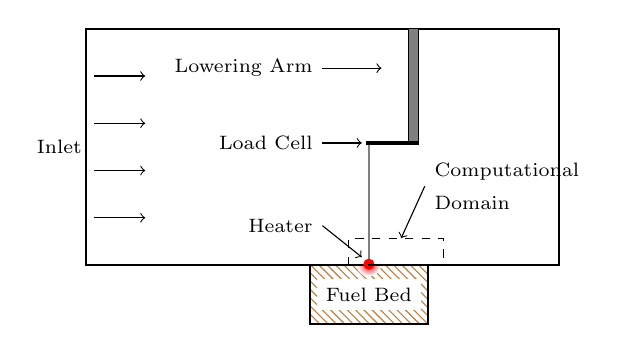
\begin{tikzpicture}
                    \filldraw[pattern=north west lines, pattern color=brown, thick] (2.84, 0)  rectangle (4.34, -.75) node[pos=0.5,rectangle,fill=white] {\scriptsize Fuel Bed};
                    \fill [draw=white,  inner color=red, outer color=white ] (3.59, 0.01) circle (0.15);
                    \filldraw[draw=black,fill=white, thick] (0, 0)      rectangle (6, 3);
                    \fill[fill=black!50] (3.58, 0) rectangle (3.61, 1.52);
                    \fill[fill=black] (3.55, 1.52) rectangle (4.23, 1.57);
                    \filldraw[draw=black, fill=black!50] (4.09, 1.57) rectangle (4.22, 3);
                    \fill[draw=red, fill=red] (3.59, 0.01) circle (0.0635);
                    \draw [<-] (3.5, 0.1) -- (3, 0.5) node[left] {\scriptsize Heater};
                    \draw [<-] (3.5, 1.55) -- (3, 1.55) node[left] {\scriptsize Load Cell};
                    \draw [<-] (3.75, 2.5) -- (3, 2.5) node[left] {\scriptsize Lowering Arm};
                    \draw[->]         (0.1, 0.6) -- (0.75, 0.6);
                    \draw[->]         (0.1, 1.2) -- (0.75, 1.2);
                    \node[right] at (-0.75, 1.5) {\scriptsize Inlet};
                    \draw[->]         (0.1, 1.8) -- (0.75, 1.8);
                    \draw[->]         (0.1, 2.4) -- (0.75, 2.4);
                    \draw[draw=black, dashed] (3.336, 0) rectangle (4.54, 0.34);
                    \draw[->]         (4.3, 1) -- (4.0, 0.34);
                    \node[right, align=left] at (4.3, 1) {\scriptsize Computational\\ \scriptsize Domain};
                \end{tikzpicture}
                }
            \caption{Diagram of the experimental wind tunnel apparatus. Air flows through the wind tunnel from left to right. The dashed region represents the domain subset used for computational efforts.}
            \label{fig:speciesWindTunnel}
        \end{figure}

    
\section{Results and Discussion}
    \label{sec:results3}
    The flaming or non-flaming ignition outcome of each test and the logistic regression results for Douglas-fir wood, oak wood, and pine wood are shown in Figure~\ref{fig:logistic_plot} for the quiescent tests. The circular markers represent the outcome of each test, either flaming or no ignition. The logistic regression for each material is shown as a solid line with the shaded regions representing the 95\% confidence interval for each regression. Douglas-fir bark, pine bark, and wheat straw are not shown in Figure~\ref{fig:logistic_plot} because flaming ignition was not observed for five tests at the maximum heater temperature of 750\si{\celsius}. The heater temperature estimated to produce 50\% ignition probability from the logistic regressions for each material is shown in Figure~\ref{tab:composition50temp}. Anecdotally, self sustained smoldering was observed for all five materials at temperatures lower than the flaming ignition temperature. The heater temperature corresponding the onset of smoldering ignition was not measured in this study. 
        \begin{figure}[htpb]
            \centering
            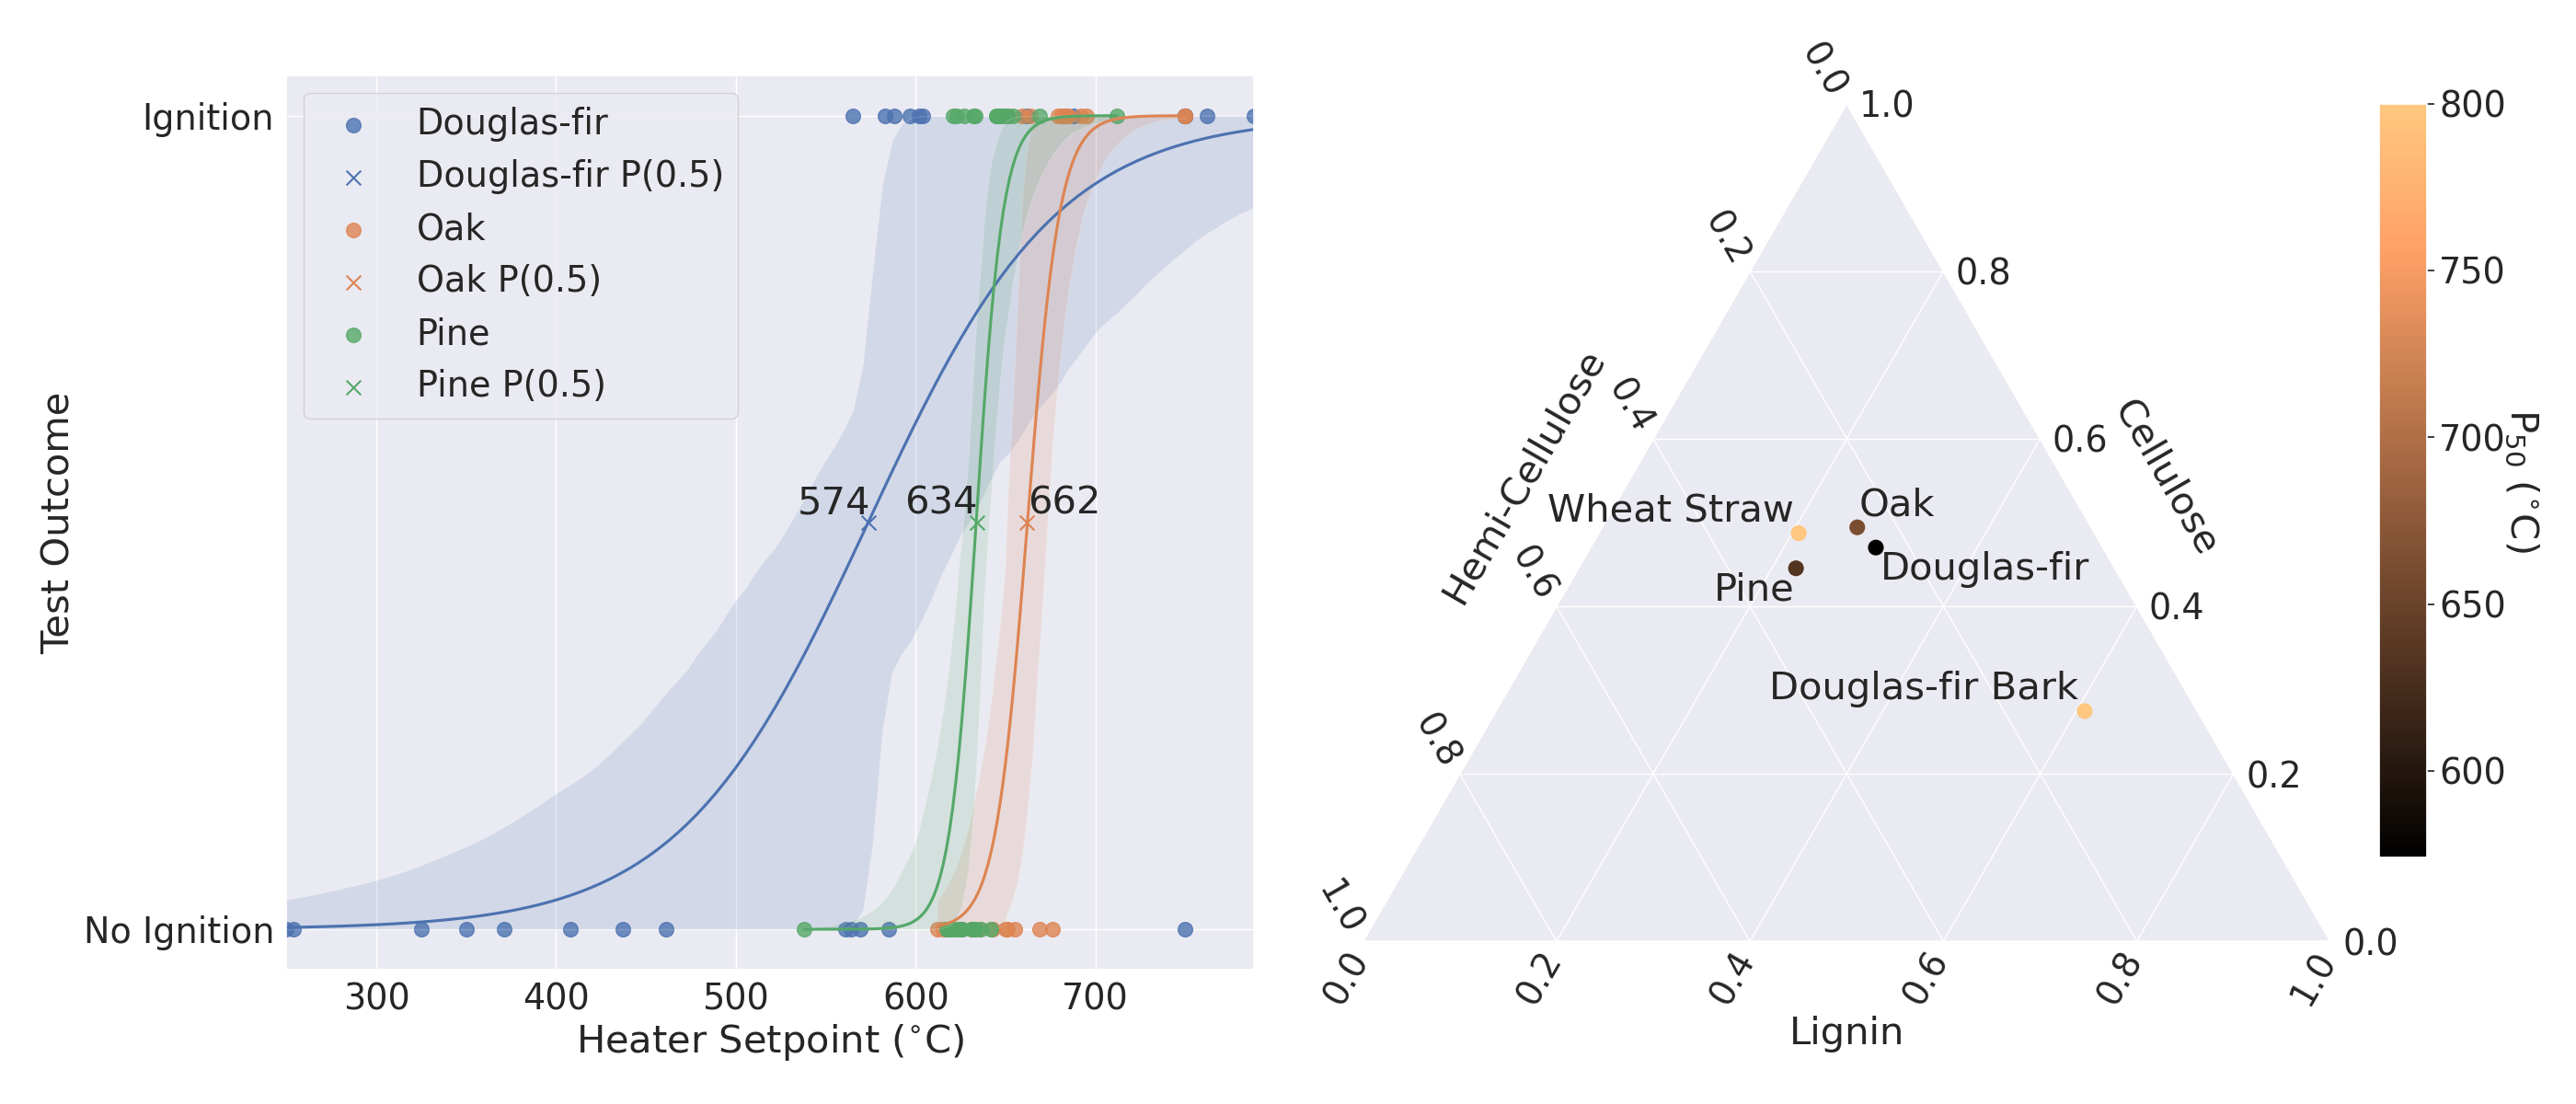
\includegraphics[width=\figureWidthSet, trim={0 0 37cm 0}, clip]{conference_results_binary.png}
            \caption{Test results for materials where flaming ignition was observed. The circular markers denote individual tests. The solid lines represent the logistic regression and the shaded zones the 95\% confidence interval with the 50\% probability of ignition labelled}
            \label{fig:logistic_plot}
        \end{figure}
    Two aspects of the ignition results are of note from the quiescent cases. As anticipated, the differences in estimated heater temperature to produce 50\% ignition probability suggest that significant differences in ignition occur across a range of materials in the same apparatus and experimental conditions. Second, the transition between no ignition and flaming ignition may become less defined (i.e., the 95\% confidence interval of the regression spans a much larger temperature range) as the ignition temperature decreases. This is significant because it may cause more difficulty in predicting the ignition of materials that ignite at lower temperatures. Lower confidence in predicting ignition for easily ignitable materials would be detrimental to the usefulness of a model or predictive tool that may be implemented from this testing methodology. It is, however, unclear if the ignition to no ignition transition in other materials of similarly low ignition temperature will behave similarly to that of Douglas-fir. Characterization of additional materials is needed to elucidate these trends.
    
    Figure~\ref{fig:composition_plot} shows the averaged cellulose, hemicellulose, and lignin concentrations for each material according to the samples recorded in the Bioenergy Feedstock Library as shown in Table~\ref{tab:composition}. The marker colors for each material correspond to the calculated 50\% ignition probability for the quiescent tests except for the wheat straw and Douglas-fir bark which are denoted as 800\si{\celsius} to indicate that the 50\% ignition probability was higher than the temperatures tested.  Note that due to scaling inherent to a ternary projection the proportion of the fuels characterized as other causes a shift in the data. For example, the wheat straw and Douglas-fir are estimated to have the same cellulose content but do not lie on the same iso-line of 44\% cellulose. Nonetheless, the relative proportions of each constituent are retained and comparisons may still be made. 
        \begin{figure}[htpb]
            \centering
            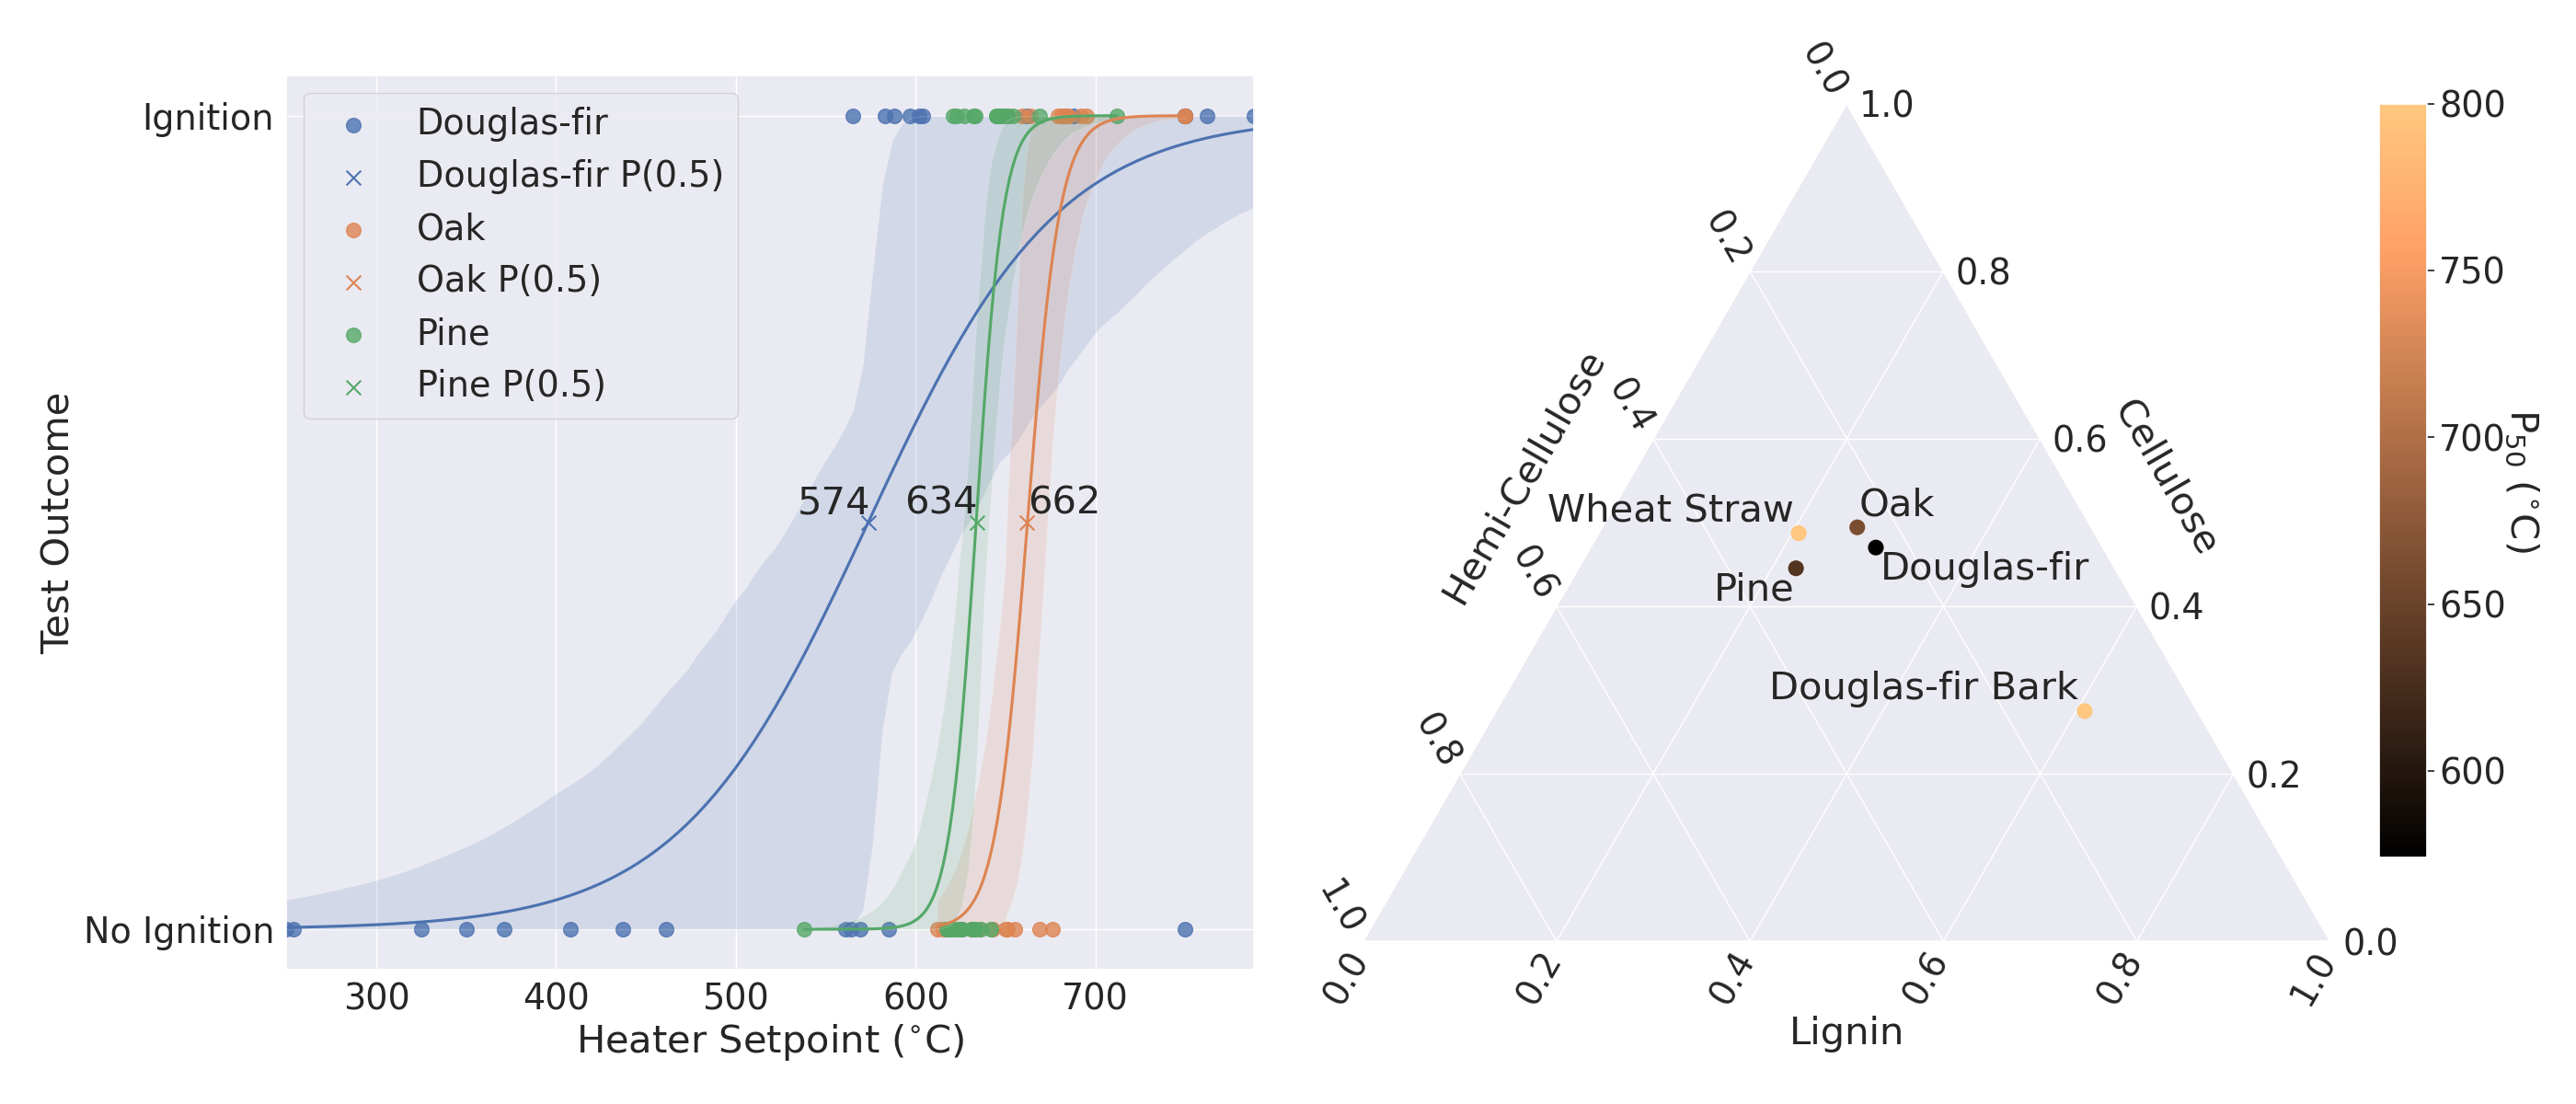
\includegraphics[width=\figureWidthSet, trim={35cm 0 0 0}, clip]{conference_results_binary.png}
            \caption{Estimated chemical composition of each material tested with the marker color representing the estimated 50\% ignition probability. Note that the materials where flaming ignition did not occur are represented as 800\si{\celsius} to show that the temperature of ignition was not achieved.}
            \label{fig:composition_plot}
        \end{figure}
    
    The 50\% ignition probability results for the 5.8\si{\meter\per\second} wind speed tests are shown in Table~\ref{tab:composition50temp} along with the results for the 0.1\si{\meter\per\second} tests. From these results there are three observations of note. First, the increase of wind lowered the threshold for ignition probability for the Douglas-fir wood and Pine wood by approximately 30\%. Second, in contrast to the Douglas-fir and Pine wood results, an increase in wind resulted in a decrease in a higher threshold for ignition.  Third, the materials that were not observed to ignite in the quiescent tests were also not observed to ignite in the presence of wind. While the trends for douglas-fir wood and pine wood match those presented in Chapter~\ref{part:manuscript2} and trends reported in other studies of pine needle ignition~\cite{Wang2017} and eucalyptus bark~\cite{Ellis2011, Ellis2015}. The decreasing ignition probability of the oak wood contradicts those observed in the aforementioned studies and this study but is not unprecedented. Ignition studies of various litter layers types ignited by various single firebrands observed a sensitivity to firebrand location where firebrands that landed on top of a fuel bed in windy conditions were less likely to cause ignition than those embedded where ignition was enhanced~\cite{Plucinski2008}. This trend was attributed to increased heat loss due to wind. In this study, however, the location of the cartridge heater was consistent across all materials, the energy is not a function of the wind speed, and the flow field around the firebrands is consistent.  
    \begin{table*}[hpbt]
        \caption{Heater temperature required for 50\% probability of ignition for the materials and conditions tested.}
        \centering
        \begin{tabular}{crrr}
            % \rowcolor{gray!50}
            Material & 0.1 \si{\meter\per\second}(\si{\celsius}) & 5.8 \si{\meter\per\second} (\si{\celsius}) & $\Delta$T (\si{\celsius})\\
            \hline
            Douglas-fir Wood & 574  & 391 & -185 \\
            Pine Wood        & 634  & 430 & -204\\
            Oak Wood         & 663  & \textgreater750 & 87\\
            Wheat Straw      & \textgreater750 & \textgreater750 & -\\
            Pine Bark        & \textgreater750 & \textgreater750 & -\\
            Douglas-Fir Bark & \textgreater750 & \textgreater750 & -
        \end{tabular}
        \label{tab:composition50temp}
    \end{table*}
    
    Taking into account the consistent ignition heat source and environmental conditions the remaining differences that may be driving factors for ignition trends are material properties. 
    The easiest material property to quantify and compare is the bulk density of the materials. However, there is no clear correlation between density and probability of ignition. Consider first the wheat straw, which was not observed to ignite at either wind speed, had a bulk density between that of pine wood and Douglas-fir wood which ignited in both wind conditions. Based on bulk density wheat straw would be anticipated to ignite at a temperature between these two materials. Similarly, oak wood has a bulk density higher than that of the douglas-fir bark and pine bark but was observed to ignite in the low wind speed cases. Clearly bulk density of the material is not a sufficient to differentiation between cases where ignition does or does not occur leaving differences in chemical composition as the remaining predictor. 
    
    Perhaps unsurprisingly, Douglas-fir bark and pine bark, with the highest lignin content, were not observed to ignite for the conditions tested. This suggests that materials with high lignin contents may be the least likely to ignite when exposed to firebrands and thus are the safest with respect to flaming ignition risk around homes. This does not, however, account for the potential for smoldering ignition and a subsequent smoldering to flaming transition that may occur. Thermogravametric analysis experiments have shown that while lignin begins to decompose at the lowest temperature of the three primary components, it decomposes at the slowest rate and at a much wider range of temperatures~\cite{Yang2007a}. It was also observed that the peak gas production of \ce{CO}, \ce{CO2}, and \ce{CH4} occurs at a higher temperatures than hemicellulose and cellulose. In contrast to Douglas-fir bark, wheat straw had the lowest estimated lignin concentration but was also not observed to ignite. When comparing wheat straw to Douglas-fir wood the higher lignin concentration suggests that Douglas-fir wood is likely to have a higher ignition temperature than wheat straw. This discrepancy is attributed to two material attributes. First, the pyrolysis process is complex and there is not a clear linear relationship between the composition of the fuel and flaming ignition. It appears that materials of different compositions are capable of producing gaseous products of near equal ignitability but the proportion of each constituent for which ignition to occurs most readily is unclear. Second, the thermal conductivity of the materials likely varies significantly which impacts the temperature gradients and mass of the material above the pyrolysis temperature, further obfuscating the effect of composition on ignition. 
    
    \section{Conclusions}
    \label{sec:conclusions3}
    Conclusions for this manuscript will go here.
    \cite{MacLean1941}.
    

    
   
%!TEX root = thesis.tex

\renewcommand{\TheTitle}{Influence of Multiple Firebrands on the Ignition of Fuel Beds}
\renewcommand{\TheAuthors}{Derek Bean, David L. Blunck}

\renewcommand{\TheAddress}{
\textbf{Status: In Preparation}
}

\PaperHeader{\TheTitle}{\TheAuthors}{\TheAddress}

\chapter{\TheTitle}
\label{part:manuscript4}

\section{Abstract}
    some text
\section{Introduction}
    The combination of increasing wildfire severity and an increase of homes in the Wildland Urban Interface (WUI) has significantly increased the occurrence of home loss due to wildfires since the turn of the century~\cite{Manzello2013}. Ignition of fuels by firebrands that leads to the loss of a structure is a primary source of home loss~\cite{Koo2010a, Syphard2019, Roberts2021}, and in some fires has been the source of 2/3 of structure ignitions~\cite{Maranghides2013NISTIgnitions}. Thus, it is important to understand the ignition of fuel beds by firebrands in order to mitigate the risk of ignition~\cite{Manzello2014}. Ideally, the understanding of the ignition process would result in a predictive model that would enable homeowners, firefighters, and other risk management personnel to determine location specific strategies for preventing ignition before and during a fire. Unfortunately, such a model does not currently exist due to critical shortfalls in the current knowledge of fuel bed ignition. 
    
    Processes that influence ignition begin within the fire when an ember (e.g., branch, bark, cone etc) is ignited and lofted into the air by wind. The combusting ember is then transported to and lands on a fuel bed near or on a structure. Energy is then transferred to the fuel bed and if the energy is sufficient the fuel bed will undergo pyrolysis and produce flammable gases which may then ignite and begin flaming. These flames may then spread and destroy the structure. Each of these processes, ember generation, transport, and ignition, require additional research before a predictive model is possible. This work focuses on the processes that occur during ignition of the fuel bed.
    
    An additional risk factor for the ignition of structures is the accumulation of embers on fuel beds. The geometry of homes often promotes the accumulation of embers by creating recirculation zones which promote the deposition of embers. The accumulation of embers poses an increased risk of home ignition in multiple ways. First, since ignition is largely a stochastic process, the more embers that land on an area the larger the probability of ignition. Second, embers that accumulate close to one another creating piles may depart more energy onto a fuel bed than a single ember alone. In work conducted by Hakes et al.~\cite{Hakes2019a} an increase in firebrand pile mass increased the total energy imparted to an instrumented surface. The increase in energy release was attained by a longer duration of energy release as the pile mass increased.
    
    The accumulation of embers near structures also requires the presence of wind which has also been shown to influence ignition. The presence of wind has been shown to decrease the threshold of ignition. In work conducted by Suzuki and Manzello~\cite{Suzuki2020a} when wind was increased from 6\si{\meter\per\second} to 8\si{\meter\per\second} the number of embers required for ignition of the wood much fuel bed decreased. Similar observations of wind lowering the ignition threshold have been observed in multiple studies with single embers. Wang et al.~\cite{Wang2017} reported decreases in ignition times as wind speed increased for hot metal particles dropped on pine needle fuel beds. Ellis reported that the addition of wind increased the threshold of fuel moisture content where ignition was observed for natural firebrands  deposited on eucalypt forest litter. The trends observed by Ellis agreed with those observed by Ganteaume et al.~\cite{Ganteaume2009} and Pulcinski and Anderson~\cite{Plucinski2008} where the addition of wind increased ignition probability. From these studies an increase of wind increases the danger of fuel bed ignition near homes but the mechanism(s) that cause the increased ignition probability are unclear. 
    
    For single firebrands it has been postulated that the primary enhancement of wind is due to increased oxygen to the ember and fuel bed. From these works it was unclear if the ignition enhancement was due to increased heat release from the ember, increased mixing and oxygen in the pyrolyzates, or some combination of both. Results from the work outlined in Chapter~\ref{part:manuscript2} show that in the presence of an ignition source where the heat release is not influenced by wind an increase of wind increases the ignition probability. The increase in ignition probability was attributed to the accumulation of pyrolysis products near the energy source (cartridge heater) suggesting that fluid flow near the ember is a significant controlling parameter for ignition. 
    
    The addition of multiple firebrands in close proximity adds additional layers of complexity with respect to both heat release and fluid dynamics.  Hakes et al.~\cite{Hakes2019a} identified re-radiation and reheating as key processes that differentiate single embers from multiple embers and have significant influence on energy deposited to the fuel bed.  The presence of multiple embers may also create disturbances in the fluid flow around the embers that influence recirculation zones and alter the ignition propensity. What is unclear from these conclusions is the magnitude of the effect that re-radiation and flow disturbances have on ignition. Understanding the magnitude of these processes on the probability of ignition is imperative to creating accurate ignition models. 
    
    With this background and motivation, the objective of this study is to quantify the influence of multiple embers on the ignition propensity of a fuel bed. It is anticipated that the results of this work will help further the understanding of the difference in ignition propensity between a single ember and multiple embers that may interact through fluid and thermal processes. A more complete understanding of these processes will enable an increased accuracy of ignition models and better protection of structures in the WUI.
    
    
\section{Methodology}
    The probability of flaming ignition for fuel beds consisting of Douglas-fir particles was measured for eight configurations of two embers in a wind tunnel. The wind tunnel was operated at either 0.5 \si{\meter\per\second} or 5.8 \si{\meter\per\second} for each test series. The wind speed was measured with a TSI-IFA300 hot wire probe. Figure~\ref{fig:multiHeaterApparatus} shows a representation of the wind tunnel, fuel bed, and the automated lowering device. Table~\ref{tab:multiHeaterConfig} shows the test matrix for each series of tests. For all of the tests the heaters were oriented perpendicular to the flow and the downstream heater was heated. For tests where both heaters were heated the temperatures of both heaters were maintained at the same temperature. 
    
    The combinations of heater spacing and hot or ambient upstream heater were chosen to represent different levels of fluid and thermal interactions between the heaters and the fuel bed. The heater spacing of five diameters was chosen such that minimal interaction between the heaters occurs as previous CFD calculations indicate that the recirculation zone of the upstream heater is approximately five diameters when the heater is in a wind of 5.8 \si{\meter\per\second} and an orientation perpendicular to the flow. Preliminary thermal calculations also indicated that the pyrolysis fronts created by each heater are unlikely to interact within previously observed times to ignition. The heater spacing of one diameter was chosen for a high level of interaction between both the fluid disturbances and thermal fronts of each ember. The one diameter spacing places the downstream heater inside the recirculation zone of the upstream heater under wind and the preliminary heat transfer calculations indicated that the thermal fronts of each heater will merge before the anticipated time to ignition. The chosen heater orientations also represent potential scenarios that may be encountered in a wildfire. The configuration with two heaters both heated is representative of a multi ember attack where the one diameter spacing approximates a firebrand pile and the five diameter spacing approximates two embers falling in close proximity but not within each others region of influence. The configuration with only the downstream heater heated is representative of an ember falling near an object (e.g., twig, rock, or cone) that disturbs the flow and may act as a heat sink for the energy deposited to the ember with the one and five diameter spacing representing an ember falling both within and outside of the region of influence of the ember. The configuration where the upstream heater is not heated and five diameters is also considered a control for comparison to previous single heater ignition results.
    
            \rowcolors{2}{gray!25}{white}
        \begin{table}[hpbt]
            \normalsize
            \caption{Test matrix}
            \centering
            \begin{tabular}{ccccr}
                \rowcolor{gray!50}
               Test Series & Heater Spacing & Upstream Heater & U\textsubscript{bulk} (\si{\meter\per\second})\\
                \hline
                1   & 1 & Ambient & 0.5 \\
                2   & 1 & Ambient & 5.8 \\
                3   & 1 & Hot     & 0.5 \\
                4   & 1 & Hot     & 5.8 \\
                5   & 5 & Ambient & 0.5 \\
                6   & 5 & Ambient & 5.8 \\
                7   & 5 & Hot     & 0.5 \\
                8   & 5 & Hot     & 5.8 \\
            \end{tabular}
            \label{tab:multiHeaterConfig}
        \end{table}
    
    The cartridge heaters used had diameters of 6.4\si{\milli\meter} and lengths of 51\si{\milli\meter}. The heater sizes were chosen to represent large firebrands with a high potential to ignite a fuel bed in a wildfire~\cite{Manzello2007}. The heater temperatures were controlled using a PID temperature controller implemented in LabVIEW. Heater temperatures ranged from 250\si{\celsius} to 750\si{\celsius}. Heater temperatures were measured using a type-K thermocouple attached to the center of each heater opposite the fuel bed.
    Controlling the temperature of the heater provides an advantage over natural burning or smoldering embers and pre-heated particles by removing the temperature variability of the heat source and enabling real time data logging of the heat source temperature. Controlling the temperature of the ember also removes some complexity of calculating the energy imparted to the fuel bed. The heater was lowered onto the fuel bed with an automated lowering device. The lowering device included a load cell and a PID controller to maintain a force equivalent to a two 10\si{\gram} firebrands throughout the experiment. To minimize flow disruptions due to apparatus the heaters were each attached to two 4-40 threaded rods that extended approximately 100\si{\milli\meter} below the load cell. 
    
         \begin{figure}[hbpt]
            \centering
            \resizebox{0.5\columnwidth}{!}{%
                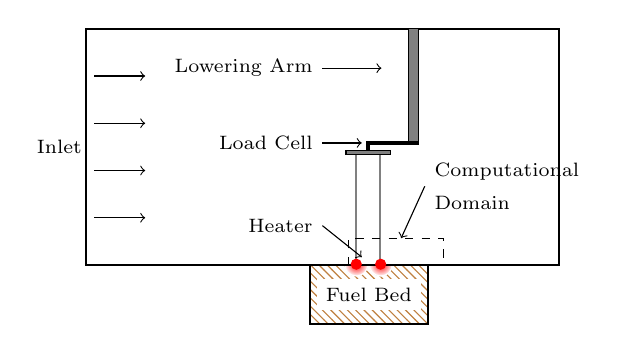
\begin{tikzpicture}
                    \filldraw[pattern=north west lines, pattern color=brown, thick] (2.84, 0)  rectangle (4.34, -.75) node[pos=0.5,rectangle,fill=white] {\scriptsize Fuel Bed};
                    \fill [draw=white,  inner color=red, outer color=white ] (3.43, 0.01) circle (0.15);
                    \fill [draw=white,  inner color=red, outer color=white ] (3.74, 0.01) circle (0.15);
                    \filldraw[draw=black,fill=white, thick] (0, 0)      rectangle (6, 3);
                    \fill[fill=black!50] (3.41, 0) rectangle (3.44, 1.40);
                    \fill[fill=black!50] (3.72, 0) rectangle (3.75, 1.40);
                    \fill[fill=black] (3.55, 1.52) rectangle (4.23, 1.57);
                    \fill[fill=black] (3.55, 1.45) rectangle (3.60, 1.52);
                    \filldraw[draw=black, fill=black!50] (3.3, 1.40) rectangle (3.86, 1.45);
                    \filldraw[draw=black, fill=black!50] (4.09, 1.57) rectangle (4.22, 3);
                   
                    \draw [<-] (3.5, 0.1) -- (3, 0.5) node[left] {\scriptsize Heater};
                    \draw [<-] (3.5, 1.55) -- (3, 1.55) node[left] {\scriptsize Load Cell};
                    \draw [<-] (3.75, 2.5) -- (3, 2.5) node[left] {\scriptsize Lowering Arm};
                    \draw[->]         (0.1, 0.6) -- (0.75, 0.6);
                    \draw[->]         (0.1, 1.2) -- (0.75, 1.2);
                    \node[right] at (-0.75, 1.5) {\scriptsize Inlet};
                    \draw[->]         (0.1, 1.8) -- (0.75, 1.8);
                    \draw[->]         (0.1, 2.4) -- (0.75, 2.4);
                    \draw[draw=black, dashed] (3.336, 0) rectangle (4.54, 0.34);
                    \draw[->]         (4.3, 1) -- (4.0, 0.34);
                    \node[right, align=left] at (4.3, 1) {\scriptsize Computational\\ \scriptsize Domain};
                    \fill[draw=red, fill=red] (3.43, 0.01) circle (0.0635);
                    \fill[draw=red, fill=red] (3.74, 0.01) circle (0.0635);
                \end{tikzpicture}
                }
            \caption{Diagram of the experimental wind tunnel apparatus. Air flows through the wind tunnel from left to right. The dashed region represents the domain subset used for computational efforts.}
            \label{fig:multiHeaterApparatus}
        \end{figure}
    
    The fuel bed material was processed from kiln dried Douglas-fir lumber. The lumber was first planed to generate shavings. The wood shavings were then granulated and screened such that the particles passed through a 2.3\si{\milli\meter} screen but not through a 1.3\si{\milli\meter} screen. The particles were then dried in an oven at 103\si{\celsius} to remove any remaining moisture content. During tests, the fuel was placed in a 140\si{\milli\meter} diameter glass container with a depth of 70\si{\milli\meter} and then inserted into the wind tunnel. The average density of the fuel beds was XX.X\si{\kilo\gram\per\cubic\meter}.
    
\section{Results and Discussion}
    The flaming ignition or non-ignition result of each test is shown in Figure~\ref{fig:multi_heater_hot_vs_ambient}. The markers show the result of each test and the the curves show the logistic regression for each of the heater configurations as defined in Table\ref{tab:multiHeaterConfig} (i.e., tests with the same wind speed, heater spacing, and upstream heater hot or ambient). The shaded regions around the curves represent the 95\% confidence intervals of each regression. The top plot in Figure~\ref{fig:multi_heater_hot_vs_ambient} shows configurations where the downstream heater is actively heated and the upstream heater is at ambient conditions. The bottom plot in Figure~\ref{fig:multi_heater_hot_vs_ambient} shows results for configurations where both heaters are actively heated to the same temperature.
        \begin{figure}[hpbt]
            \centering
            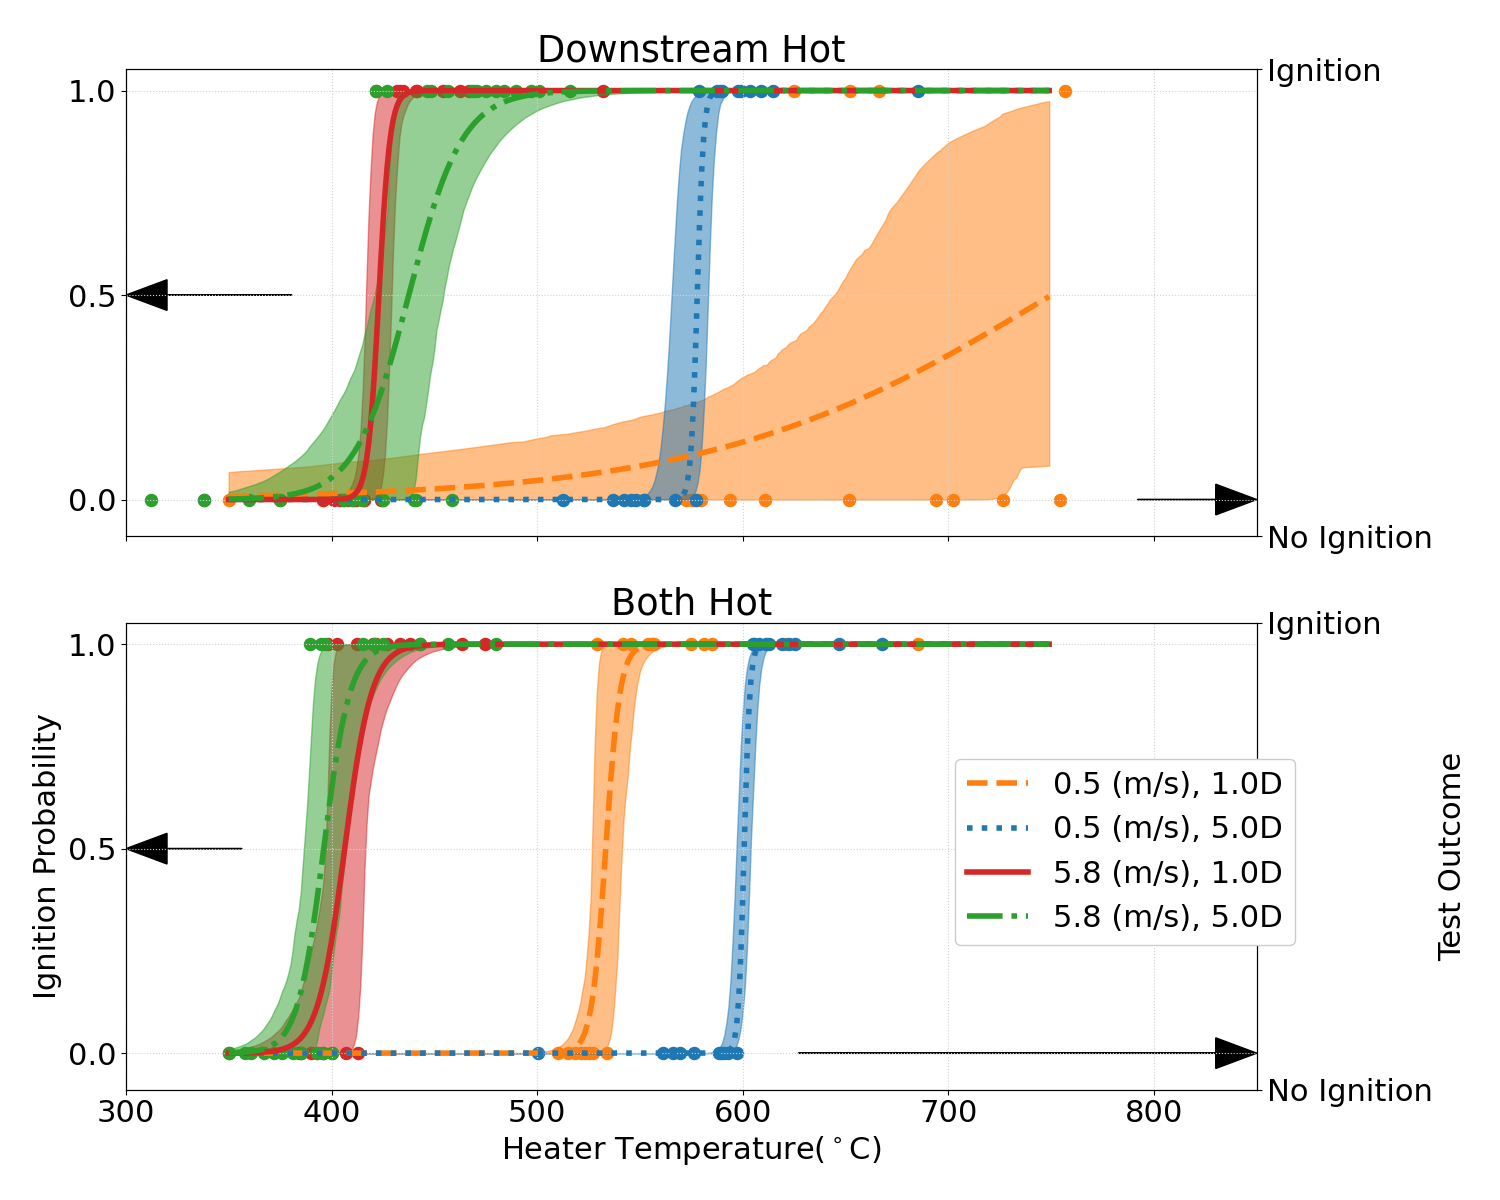
\includegraphics[width=0.75\columnwidth]{Figures/multi_heater_plot.png}
            \caption{Ignition or no ignition outcomes of tests with different heater configurations. The circular markers indicate outcomes of individual tests and the curves represent logistic regressions of each test series. The shaded region shows the 95\% confidence interval for each regression.}
            \label{fig:multi_heater_hot_vs_ambient}
        \end{figure}
    Table~\ref{tab:multiFiftyTemp} shows the heater temperatures estimated to result in a 50\% ignition probability from the logistic regressions shown in Figure~\ref{fig:multi_heater_hot_vs_ambient} with the bounds of the 95\% confidence intervals included. Temperature values for the corresponding wind speed and orientation from the single heater study in Chapter~\ref{part:manuscript2} are shown in the column titled "Single" for comparison. 
        \rowcolors{2}{gray!25}{white}
        \begin{table}[hpbt]
            \normalsize
            \caption{Heater temperature required to achieve 50\% ignition probability for the configurations tested with 95\% confidence intervals shown in parentheses. The single heater column shows the values from the study in Chapter~\ref{part:manuscript2} for a single heater.}
            \centering
            \begin{tabular}{ccrrr}
                \rowcolor{gray!50}
               U\textsubscript{bulk} (\si{\meter\per\second}) & Spacing (D) & Ambient (\si{\celsius})& Heated (\si{\celsius}) & Single (\si{\celsius})\\
                \hline
                0.5  & 1 & 750 (644, 850) & 533 (527, 541) & 571\\
                0.5  & 5 & 578 (565, 583) & 601 (597, 604) & 571\\
                5.8  & 1 & 423 (417, 429) & 406 (397, 416) & 399\\
                5.8  & 5 & 438 (421, 454) & 396 (387, 407) & 399
            \end{tabular}
            \label{tab:multiFiftyTemp}
        \end{table}
        
    Considering first the cases where both heaters are actively heated there are three observations of note. First, in both the one and five heater diameter spacing cases an increase in wind from 0.5\si{\meter\per\second} to 5.8\si{\meter\per\second} resulted in a lower temperature threshold for ignition. These results are consistent with the results for a single heater presented in Chapter~\ref{part:manuscript2} and are attributed to an increased residence time of pyrolyzates near the heater in recirculation zones enabling ignition at lower temperatures. Second, for the 0.5\si{\meter\per\second} wind speed tests decreasing the heater spacing from five heater diameters to one heater diameter resulted in an 11\% decrease in the temperature required for 50\% ignition probability. The shift in ignition probabilities is attributed to increased heat transfer between the closely spaced heaters. For tests that were conducted with heater temperatures near the 50\% ignition temperature a shift in the model of ignition occurred. For cases where the heaters where spaced five diameters apart ignitions occurred within $\approx$1\si{\second} of the heaters being lowered. Similar ignition times were characteristic of the single diameter spaced heaters at higher temperatures. However, for the single diameter spaced heaters ignitions with heater temperatures near the 50\% ignition limit did not typically ignite until the pyrolysis fronts from both heaters merged. Ignition then occurred in the plume of pyrolyzates between the heaters and anchored to the fuel bed. This phenomena is attributed to .... In contrast to the differences in ignition at a wind speed of 0.5\si{\meter\per\second} the differences in ignition probability were not statistically significant at 5.8\si{\meter\per\second}. This suggests that the enhanced heat transfer between the cartridge heaters is not influential in windy conditions. Anecdotally, in cases under wind ignitions were to occur on the upstream side of the upstream cartridge heater suggesting that ignition is more favorable in the recirculation zones on the upstream side of the heater even with the addition of heat and pyrolysis 
   
    Now considering the cases where the only the upstream heater was actively heated there are three observations of note. Similar to the dual hot and single heater results from Chapter~\ref{part:manuscript2} an increase of wind from 
    
\section{Conclusions}
    some text
%%!TEX root = thesis.tex

\chapter{Results \& Discussion}
\label{part:results}
The preceding chapters of this document presented findings from studies evaluating the influence of various parameters on the probability of ignition of fuel beds in wild fires. These studies were conducted to address the specific objectives of this work and to add to the current body of knowledge regarding ignition with the overall goal of facilitating a model for quickly and accurately predicting ignition risk to reduce the number of homes lost to wildfires. The specific objectives of this work are as follows:
        \begin{enumerate}
            \item Determine the effects of particle morphology on ignition propensity
            \item Ascertain ignition dependence on heating location(s), mode, and rate
            \item Identify and quantify the influence of environmental conditions on ignition propensity.
            \item Identify the influence of fuel bed chemical composition on flaming ignition.
        \end{enumerate}
The conclusions of each effort are restated in the following sections followed by a discussion of the implications of the results as they pertain to each specific objective and the overall objective of this work.

\section{Particle Size}
        \begin{enumerate}
            \item 
                Smaller particles ignite more readily in porous beds than larger particles when heat transfer from the heater is primarily through conduction. This was evident by higher ignition probabilities, in general, of the smaller particles for a fixed heater temperature. As particle sizes increase radiant heat transfer becomes more important and fuel beds with larger particles were more likely than smaller particles to ignite at extended times (\textgreater 100\si{\second}) due to the increased importance of radiant ignition. 
            \item
                Douglas-fir plates ignite at times where conduction is the dominant mode of heat transfer (\textless 10\si{\second}) due to the higher thermal conductivity of the solid plates. The ignition probability of plates was the most similar to the larger particle, in particular at lower heater temperatures, due to dispersed heating of the porous fuel bed through radiation and the increased thermal conductivity of the plates creating similar temperature profiles. The rise in ignition probability  over a smaller heater temperature range time with temperature results from more consistent contact between the heater and plate surface.
            \item 
                Heat flux delivered to the fuel bed, when compared to heater temperature, is more indicative of ignition likelihood and ignition time for porous fuel beds. Heat flux is a more significant predictor of ignition because it captures differences in heat transfer modes and particle contact that heater temperature values do not. While this finding is not new, what is novel is that the mixed mode of heating (conduction and radiation) has a significant impact on the flaming ignition of fuel beds.
            \item 
                Consideration of the transport characteristics of pyrolyzate gases near the high temperature source can be important for more fully predicting ignition propensity. A \textit{Da} of ignition, in relation to the measured heat flux and thermal diffusivity of the fuel beds, is a promising relationship for predicting ignition for the porous fuel beds.  
        \end{enumerate}

\section{Wind Speed}
        \begin{enumerate}
            \item
            An increase in wind speed above quiescent conditions reduces the temperature required for the flaming ignition of a fuel bed. For example, an increase in wind speed of 3.5\si{\meter\per\second} from quiescent increases the ignition probability of a fuel bed from under 30\% to roughly 100\%. However, a linear increase in wind speed does not result in a linear increase in ignition probability. Thresholds in wind speed exist above which temperatures required to achieve ignition actually increase. For example, when the wind is oriented 45\si{\degree} from the heater centerline increasing the wind from quiescent to 3.5\si{\meter\per\second} reduces the temperature required for ignition probability by 30\%. However, increasing the wind speed from quiescent to 5.8\si{\meter\per\second} reduces the temperature required for ignition by only 25\%. Presumably these thresholds occur because of reductions in residence time. 
            
            \item The temperatures at which ignition occurs for porous fuel beds is sensitive to the orientation of a firebrand relative to the wind direction. Higher temperatures are typically required for ignition for a heater parallel to the flow compared to 45\si{\degree} and perpendicular to the flow. This sensitivity attributed to differences in recirculation zones and residence times of air and pyrolyzates near the hottest region of the heater. Thus, predictions of ignition probabilities that consider wind may need to include both wind speed and orientation to obtain sufficient accuracy.
            
            \item Times to flaming ignition of porous fuel beds are sensitive to the firebrand/heater angle in the presence of wind.
            The parallel heater orientation ignites at the longest time followed by the 45\si{\degree} case with the perpendicular cases igniting in the shortest amount of time. High speed images indicate that ignition typically occurs in regions where recirculation zones occur, as shown in CFD calculations. The heightened propensity to ignition is attributed to increased residence times of pyrolyzates in the recirculation zones as supported by calculations.
        \end{enumerate}
    The conclusions of this work show that ignition is favored when a firebrand(s) land on a fuel bed under wind speeds and orientations that promote greater residence times of pyrolyzates near a high temperature region of firebrands. It was observed that increases of wind speed, of a magnitude that may commonly occur during wildfires, can increase the probability of fuel bed ignition from very unlikely to a near certainty regardless of the ember orientation to the wind. This highlights the increased risk of spot fires due to ignition of fuel beds that accompanies wind in a wildfire. 

\section{Species}

\section{Ember Interactions}

\section{Overall model}
%!TEX root = thesis.tex

\chapter{Conclusions \& Future Work}
\label{part:conclusion}
\label{part:results}
The preceding chapters of this document presented findings from studies evaluating the influence of various parameters on the probability of ignition of fuel beds in wild fires. These studies were conducted to address the specific objectives of this work and to add to the current body of knowledge regarding ignition with the overall goal of facilitating a model for quickly and accurately predicting ignition risk to reduce the number of homes lost to wildfires. The specific objectives of this work are as follows:
        \begin{enumerate}
            \item Determine the effects of particle morphology on ignition propensity
            \item Ascertain ignition dependence on heating location(s), mode, and rate
            \item Identify and quantify the influence of environmental conditions on ignition propensity.
            \item Identify the influence of fuel bed chemical composition on flaming ignition.
        \end{enumerate}
The conclusions of each effort are restated in the following sections followed by a discussion of the implications of the results as they pertain to each specific objective and the overall objective of this work.

\section{Particle Size}
        \begin{enumerate}
            \item 
                Smaller particles ignite more readily in porous beds than larger particles when heat transfer from the heater is primarily through conduction. This was evident by higher ignition probabilities, in general, of the smaller particles for a fixed heater temperature. As particle sizes increase radiant heat transfer becomes more important and fuel beds with larger particles were more likely than smaller particles to ignite at extended times (\textgreater 100\si{\second}) due to the increased importance of radiant ignition. 
            \item
                Douglas-fir plates ignite at times where conduction is the dominant mode of heat transfer (\textless 10\si{\second}) due to the higher thermal conductivity of the solid plates. The ignition probability of plates was the most similar to the larger particle, in particular at lower heater temperatures, due to dispersed heating of the porous fuel bed through radiation and the increased thermal conductivity of the plates creating similar temperature profiles. The rise in ignition probability  over a smaller heater temperature range time with temperature results from more consistent contact between the heater and plate surface.
            \item 
                Heat flux delivered to the fuel bed, when compared to heater temperature, is more indicative of ignition likelihood and ignition time for porous fuel beds. Heat flux is a more significant predictor of ignition because it captures differences in heat transfer modes and particle contact that heater temperature values do not. While this finding is not new, what is novel is that the mixed mode of heating (conduction and radiation) has a significant impact on the flaming ignition of fuel beds.
            \item 
                Consideration of the transport characteristics of pyrolyzate gases near the high temperature source can be important for more fully predicting ignition propensity. A \textit{Da} of ignition, in relation to the measured heat flux and thermal diffusivity of the fuel beds, is a promising relationship for predicting ignition for the porous fuel beds.  
        \end{enumerate}

\section{Wind Speed}
        \begin{enumerate}
            \item
            An increase in wind speed above quiescent conditions reduces the temperature required for the flaming ignition of a fuel bed. For example, an increase in wind speed of 3.5\si{\meter\per\second} from quiescent increases the ignition probability of a fuel bed from under 30\% to roughly 100\%. However, a linear increase in wind speed does not result in a linear increase in ignition probability. Thresholds in wind speed exist above which temperatures required to achieve ignition actually increase. For example, when the wind is oriented 45\si{\degree} from the heater centerline increasing the wind from quiescent to 3.5\si{\meter\per\second} reduces the temperature required for ignition probability by 30\%. However, increasing the wind speed from quiescent to 5.8\si{\meter\per\second} reduces the temperature required for ignition by only 25\%. Presumably these thresholds occur because of reductions in residence time. 
            
            \item The temperatures at which ignition occurs for porous fuel beds is sensitive to the orientation of a firebrand relative to the wind direction. Higher temperatures are typically required for ignition for a heater parallel to the flow compared to 45\si{\degree} and perpendicular to the flow. This sensitivity attributed to differences in recirculation zones and residence times of air and pyrolyzates near the hottest region of the heater. Thus, predictions of ignition probabilities that consider wind may need to include both wind speed and orientation to obtain sufficient accuracy.
            
            \item Times to flaming ignition of porous fuel beds are sensitive to the firebrand/heater angle in the presence of wind.
            The parallel heater orientation ignites at the longest time followed by the 45\si{\degree} case with the perpendicular cases igniting in the shortest amount of time. High speed images indicate that ignition typically occurs in regions where recirculation zones occur, as shown in CFD calculations. The heightened propensity to ignition is attributed to increased residence times of pyrolyzates in the recirculation zones as supported by calculations.
        \end{enumerate}
    The conclusions of this work show that ignition is favored when a firebrand(s) land on a fuel bed under wind speeds and orientations that promote greater residence times of pyrolyzates near a high temperature region of firebrands. It was observed that increases of wind speed, of a magnitude that may commonly occur during wildfires, can increase the probability of fuel bed ignition from very unlikely to a near certainty regardless of the ember orientation to the wind. This highlights the increased risk of spot fires due to ignition of fuel beds that accompanies wind in a wildfire. 

\section{Species}

\section{Ember Interactions}
        \begin{enumerate}
            \item An increase of wind speed from 0.5\si{\meter\per\second} to 5.8\si{\meter\per\second} reduced the temperature required for ignition for all heater configurations. The decrease in ignition temperature required ranged from 20\% to 60\% depending on the heater configuration. 
            
            \item At wind speeds of 5.8\si{\meter\per\second} the ignition threshold is largely independent of the heater configuration. This lack of sensitivity is attributed to the ignition being controlled by the fluid dynamics around the firebrand surrogates. Under wind ignition is largely controlled by the propensity of pyrolysis products to accumulate in recurculation zones and independent of thermal interactions with nearby objects whether they are energy sources or sinks. 
            \item At wind speeds of 0.5\si{\meter\per\second} the ignition threshold is dependent on the firebrand surrogate configuration. For example, when the firebrand were spaced one diameter apart the difference between ignition thresholds when the upstream firebrand is inert or an energy source is 34\%. When the firebrand surrogates were spaced such that they did not thermally interact (five diameters apart) the difference in ignition threshold was 4\%. Thus, at low wind speeds or in quiescent conditions ignition is sensitive to thermal interactions with nearby objects. Ignition is promoted if nearby objects supply energy and inhibited if energy sinks are nearby. 
            
            \item In configurations where the firebrand surrogate is downstream of an inert flow obstacle ignition may occur as a smoldering to flaming transition. The smoldering to flaming transition appears to be facilitated by either accumulation of pyrolysis gases in the downstream edge of the flow obstruction or by the formation of an overhang as the fuel bed recedes underneath the obstruction. This phenomena produces ignition at similar temperatures to other configurations and may not be important for ignition predictions but may be of interest to smoldering research. 
        \end{enumerate}

\section{Overall model}
    The overall objective of this work is to identify parameters and processes that control the ignition of a fuel bed when an ember lands on it with an anticipated impact of enabling the creation of a simplified model that may be used quickly determine the likelihood of ignition. To evaluate the effectiveness of this work in meeting those goals a model was created to predict ignition. The model was then applied to results of other studies that utilized different fuel bed materials and ignition sources to determine cross study applicability.
    
    
    
    

\section{Future Work}

\addcontentsline{toc}{chapter}{Bibliography}

\newpage

\printbibliography[]


%% INCLUDE IF YOU NEED AN APPENDIX

% \newpage
%\appendix
%\input{appendixA.tex}

\end{document}
